% !TEX encoding = UTF-8 Unicode
\documentclass[a4paper]{article}

\usepackage{color}
\usepackage[obeyspaces]{url}
\usepackage[T1]{fontenc} % enable Cyrillic fonts
\usepackage[utf8]{inputenc} % make weird characters work
\usepackage{graphicx}
% \usepackage[margin=1.5in]{geometry}
\usepackage[table]{xcolor}

\usepackage[english,serbian]{babel}
%\usepackage[english,serbianc]{babel} 
\usepackage{float}


\PassOptionsToPackage{obeyspaces}{url}
\usepackage[unicode]{hyperref}
\hypersetup{colorlinks,citecolor=green,filecolor=green,linkcolor=blue,urlcolor=blue}

\usepackage{listings}
\renewcommand\lstlistingname{Kod}
\renewcommand\lstlistlistingname{Kodovi}

\definecolor{mygreen}{rgb}{0,0.6,0}
\definecolor{mygray}{rgb}{0.5,0.5,0.5}
\definecolor{mymauve}{rgb}{0.58,0,0.82}

\lstset{ 
  backgroundcolor=\color{white},   % choose the background color; you must add \usepackage{color} or \usepackage{xcolor}; should come as last argument
  basicstyle=\scriptsize\ttfamily,        % the size of the fonts that are used for the code
  breakatwhitespace=false,         % sets if automatic breaks should only happen at whitespace
  breaklines=true,                 % sets automatic line breaking
  captionpos=b,                    % sets the caption-position to bottom
  commentstyle=\color{mygreen},    % comment style
  deletekeywords={...},            % if you want to delete keywords from the given language
  escapeinside={\%*}{*)},          % if you want to add LaTeX within your code
  extendedchars=true,              % lets you use non-ASCII characters; for 8-bits encodings only, does not work with UTF-8
  firstnumber=1,                % start line enumeration with line 1000
  frame=single,	                   % adds a frame around the code
  keepspaces=true,                 % keeps spaces in text, useful for keeping indentation of code (possibly needs columns=flexible)
  keywordstyle=\color{blue},       % keyword style
  language=Python,                 % the language of the code
  morekeywords={*,...},            % if you want to add more keywords to the set
  numbers=left,                    % where to put the line-numbers; possible values are (none, left, right)
  numbersep=5pt,                   % how far the line-numbers are from the code
  numberstyle=\tiny\color{mygray}, % the style that is used for the line-numbers
  rulecolor=\color{black},         % if not set, the frame-color may be changed on line-breaks within not-black text (e.g. comments (green here))
  showspaces=false,                % show spaces everywhere adding particular underscores; it overrides 'showstringspaces'
  showstringspaces=false,          % underline spaces within strings only
  showtabs=false,                  % show tabs within strings adding particular underscores
  stepnumber=2,                    % the step between two line-numbers. If it's 1, each line will be numbered
  stringstyle=\color{mymauve},     % string literal style
  tabsize=2,	                   % sets default tabsize to 2 spaces
  title=\lstname                   % show the filename of files included with \lstinputlisting; also try caption instead of title
}

\begin{document}

\title{[RM] Pitanja i odgovori}

\author{Momir Adžemović}

\date{11.~maj 2020.}

\maketitle

\tableofcontents

\newpage

\section{Komponente mreže, tipovi mreža, primeri mreža, mreže prema dimenziji, međumreže}
    \subsection{Komponente mreže}
        Mrežu možemo da posmatrama kao neusmereni graf (teoretski mreža može da bude usmereni graf tj.
        veza slanja podataka između dva čvora može da bude jednosmerna). Komponente mreže su:
        \begin{itemize}
            \item \underline{Aplikacija}, koristi mrežu i predstavlja komponentu lista grafa mreže.\\
                  Primer: Skype, Itunes, Minecraft...
            \item \underline{Računar}, podržava aplikaciju predstavlja završni čvor u grafu mreže.\\
                  Primer: Dekstop računar, laptop, telefon...
            \item \underline{Ruter}, prosleđuje poruke između čvorova i predstavlja unutrašnji čvor grafa mreže.\\
                  Primer: kablovski/DSL modem, ...
            \item \underline{Veza ili kanal}, spaja čvorove i predstavlja granu u čvoru.\\
                  Tipovi: Žičani i bežični.
        \end{itemize}
        \begin{figure}[H]
            \begin{center}
                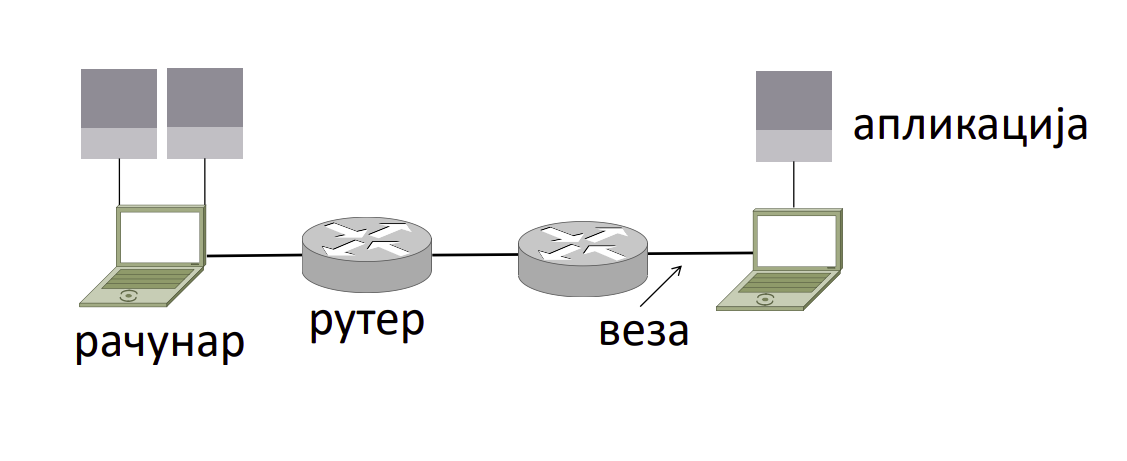
\includegraphics[width=100mm,height=50mm]{Slike/komponente_mreze.png}
            \end{center}
        \end{figure}
    \subsection{Tipovi mreža}
        \begin{itemize}
            \item \textbf{Puni dupleks} - Mogu da se šalju podaci u oba smera istovremeno.\\
                  Primer: Telefon.
            \item \textbf{Polu dupleks} - Mogu da se šalju podaci u oba smera, ali ne istovremeno.\\
                  Primer: Voki-toki.
            \item \textbf{Simpleks} - Mogu samo da se šalju ili samo da se primaju podaci.\\
                  Primer: Tastatura, monitor.
        \end{itemize}
    \subsection{Primeri mreža}
        \begin{itemize}
            \item WiFi (802.11) 
            \item Poslovne / Ethernet 
            \item ISP (Internet Service Provider) 
            \item Kablovska / DSL 
            \item Mobilna telefonija (2G, 3G, 4G, 5G) 
            \item Bluetooth 
            \item Telefon 
            \item Sateliti 
            \item ...
        \end{itemize}
    \subsection{Mreže prema dimenziji}
        \begin{itemize}
            \item \textbf{PAN (Personal Area Network)} - Odnosi se na jednu osobu.\\
                  Primer: bluetooth.
            \item \textbf{LAN (Local Area Network)} - Odnosi se na mrežu u okviru neke zgrade.\\
                  Primer: WiFi, Ethernet.
            \item \textbf{MAN (Metropolitan Area Network)} - Odnosi se na mrežu na nivou nekog grada,
                  univerziteta ili regiona.\\
                  Primer: kablovksa, DSL .
            \item \textbf{WAN (Wide Area Network)} - Odnosi se na mrežu na nivou neke velike geografske površine.\\
                  Primer: veliki ISP (Telekom, SBB).
            \item \textbf{Internet}.
        \end{itemize}
    \subsection{Međumreža}
        \textbf{Međumreža (eng. internetwork) ili internet (malim početnim slovom)} je mreža koja
        se dobija povezivanjem više različitih mreža. Internet (velikim slovom) je internet 
        koji svi mi koristimo. \\
        \indent Intuitivno spajanjem LAN i WAN ili dva LAN-a dobijamo međumrežu. 
        Postoji dogovor oko terminologije međumreže:
        \begin{itemize}
            \item Ako dve različite institucije razvijaju dva različita dela mreže, 
                  onda to nazivamo međumreža. 
            \item Ako se dva dela mreže razlikuju u tehnologiji izgradnje, onda to nazivamo međumreža.
        \end{itemize} 

\section{Protokoli i slojevi}
    Šta sve treba mreža da radi za korisnike?
    \begin{itemize}
        \item Pravi i prekida konekciju;
        \item Pronalazi putanju za transfer podataka;
        \item Pouzdano šalje podatke;
        \item Šalje podatke proizvolje veličine;
        \item Brzina slanja se prilagođava mogućnosti mreže;
        \item Omogućava siguran prenos tokom transakcije;
        \item Omogućava dodavanje čvorova
        \item ...
    \end{itemize}
    Neki od ovih zahteva su apstraktniji od drugih što je jedan od motiva za raslojavanje.\\
    \indent Prve verzije mreža su pravljenje tako da hardver ima prioritet u odnosu na softver. 
    To više nije moguće, jer je mreža previše kompleksna. Kako bi se smanjila kompleksnost mreže, 
    struktura mreže je ogranizovana kao stek slojeva (nivoa). Svrha svakog sloja (sem aplikativnog 
    čija je svrha da omogući usluge korisniku) je da omogući određene servise višem sloju.\\

    \textbf{Internet sloj} je grupa protokola i mehanizama koji čine nekakvu funkcionalnu celinu.\\
    \indent \textbf{Protokoli} predstavljaju skup pravila koji se poštuju u komunikaciji.
    Primer: http, ftp, smtp, tcp, udp, ip, 802.3, 802.11 \dots\\
    \indent \textbf{Enkapsulacija} je mehanizam u kome svaki sloj prima poruku od višeg sloja i 
    obmotava ga okvirom koji sadrži informacije vezane za taj sloj i prosleđuje nižem sloju. \\

    Primer: Šalje se HTTP zahtev sa aplikativnog sloja koji koristi TCP protokol transportnog sloja. 
    U transportnom sloju se podaci HTTP zahteva obmotavaju u segment koji sadrži dodatne informacije, 
    pored HTTP zahteva, i prosleđuje taj segment mrežnom (nižem) sloju. Mrežni sloj obmotava segment 
    u paket i prosleđuje paket sloju veze koristeći IP protokol. Sloj veze obmotava paket u okvir 
    koristeći određeni protokol i prosleđuje fizičkom sloju. Neka je taj protokol 802.11 (bežična mreža). 
    Fizički sloj prenosi podatke kao tok bitova. Niz ovih protokola čini (od najvišeg ka najnižem)
    jedan konkretan stek protokola.
    \begin{figure}[H]
        \begin{center}
            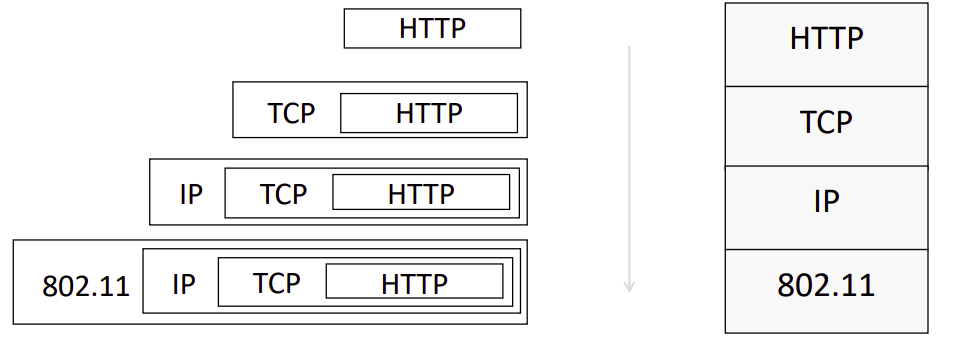
\includegraphics[width=100mm,height=50mm]{Slike/enkapsulacija.png}
        \end{center}
    \end{figure}
    \indent Kako jedan niži sloj može da uslužuje više različitih slojeva na višem nivou, 
    onda mora da postoji neki mehanizam demultipleksiranja kako bi primalac mogao
    da raspakuje poruku do aplikativnog sloja. Preko TCP porta možemo odrediti koji protokol
    se uslužuje na aplikativnom sloju (primer. http port je 80). Preko IP polja možemo odrediti
    da li se koristi TCP ili UDP (ili neki treći manje poznati). Preko tipa medijuma može se 
    odrediti koji protokol se koristi na mrežnom nivou.
    \begin{figure}[H]
        \begin{center}
            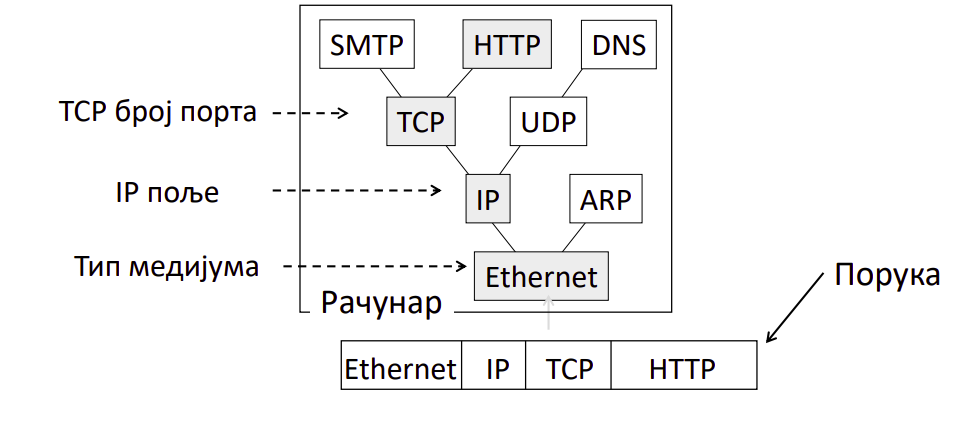
\includegraphics[width=100mm,height=50mm]{Slike/demultipleksiranje.png}
        \end{center}
    \end{figure}
    \noindent \textbf{Prednosti raslojavanja:}
    \begin{itemize}
        \item Prikrivanje informacija.
        \item Nezavisnost višeg sloja od nižeg sloja 
              (HTTP radi uvek isto, nezavisno od toga da li koristimo wifi ili ethernet).
        \item Laka konverzija poruka (primer: Oba čvora u regionu povezani žičano i koriste ethernet,
              ali da bi se poslala poruka potrebno je u nekom trenutku prenositi podatke Preko
              brežične mreže).
    \end{itemize}
    \textbf{Mane raslojavanje:}
    \begin{itemize}
        \item Povećani troškovi memorije (manje bitno za duže poruke).
        \item Prikrivanje informacija (prednost i mana). Generalno korisno, ali možda neke aplikacije
              žele da znaju da li se podaci prenose preko kabla ili bežično.
    \end{itemize}

\section{Referentni modeli protokola i slojeva, jedince podataka, organizacije za standarde.}
    \subsection{Referentni modeli protokola i slojeva}
        Potrebno je izvršiti podelu funkcionalnosti na slojeve. Koja funkcionalnost pripada kom sloju?
        Dva najpoznatija referentna modela su TCP/IP referentni model koji je dobio ime po 
        popularnim protokolima TCP i IP, i OSI (Open System Interconnection) referentni model.
        
        \subsubsection{OSI model}
            \begin{figure}[H]
                \begin{center}
                    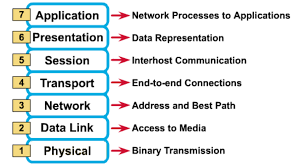
\includegraphics[width=100mm,height=50mm]{Slike/osi_model.png}
                \end{center}
            \end{figure}
            \noindent \textbf{Referentni OSI model je zasnovan na sledećim principima:}
            \begin{enumerate}
                \item Tamo gde je potrebna posebna apstrakcija treba da se napravi poseban sloj.
                \item Svaki sloj treba da ima svoju dobru definisanu funkciju.
                \item Svaki sloj treba da se bira na osnovu već poznatih standardizovanih protokola.
                \item Granice slojeva treba da se izaberu tako da prenos podataka sa sloja na sloj 
                      minimalan.
                \item Broj slojeva treba da bude dovoljno veliki da se različite funkcije nalaze 
                      na različitim slojevima, ali i dovoljno mali da sistem ne bude glomazan.
            \end{enumerate}
            \textbf{Slojevi (od najnižeg):}
            \begin{enumerate}
                \item \textbf{Fizički sloj:} Prenosi bitove preko komukacionog kanala.
                \item \textbf{Sloj veze podataka:} Prenosi okvire na nivou kanala
                      sa mogućom proverom greške i evetualnim ispravkama ili retransmisijom.
                \item \textbf{Mrežni sloj:} Prenosi pakete na nivou mreže preko rutera.
                      Na ovom sloju se vrši rutiranje.
                \item \textbf{Transportni sloj:} Prenosi segmente podataka od pošiljaoca do primaoca 
                      (eng. end-to-end layer).
                \item \textbf{Sloj sesije:} Omogućava različitim mašinama da uspostavljaju sesije između njih.
                \item \textbf{Sloj prezentacije:} Odgovoran za sintaksu i semantiku informacija koje se prenose.
                \item \textbf{Aplikativni sloj:} Pruža usluge krajnjim korisnicima.
            \end{enumerate}
        
        \subsubsection{TCP/IP model}
            \begin{figure}[H]
                \begin{center}
                    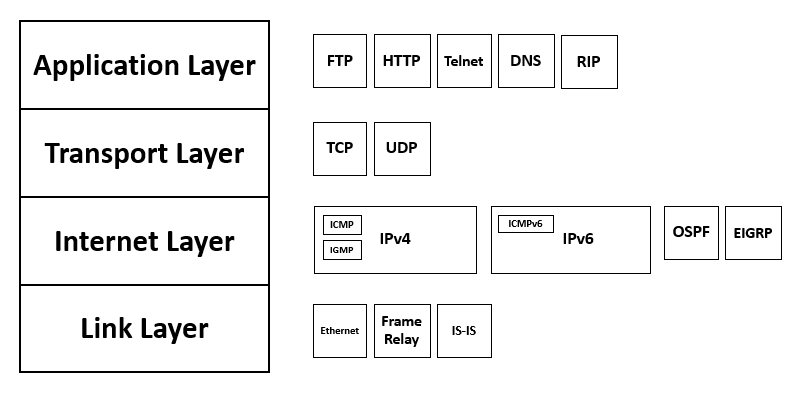
\includegraphics[width=100mm,height=50mm]{Slike/tcpip_model.png}
                \end{center}
            \end{figure}
            \textbf{Slojevi (od najnižeg):}
            \begin{enumerate}
                \item \textbf{Sloj veze:} Ne predstavlja konkretno sloj, već interfejs. 
                      Definiše kako koja veza radi.
                \item \textbf{Internet sloj:} Odgovara sloju veza za OSI model.
                \item \textbf{Transportni sloj:} Odgovara transportnom sloju za OSI model.
                \item \textbf{Aplikativni sloj:} Najviši sloj koji predstavlja interfejs ka korisnicima.
            \end{enumerate}
            \begin{figure}[H]
                \begin{center}
                    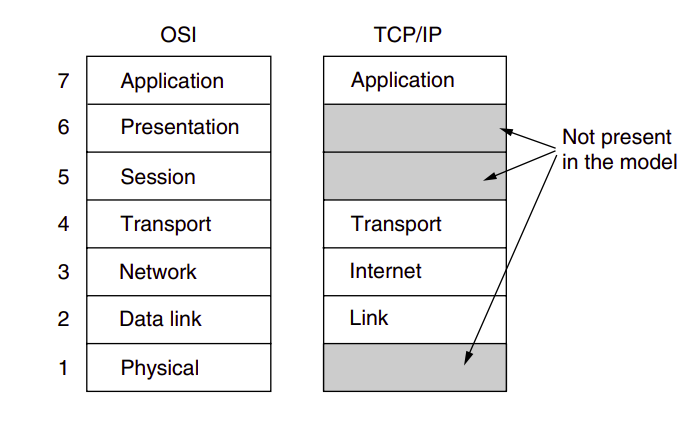
\includegraphics[width=100mm,height=50mm]{Slike/osi_vs_tcpip.png}
                \end{center}
            \end{figure}

            \newpage
            \textbf{Protokoli:}
            \begin{figure}[H]
                \begin{center}
                    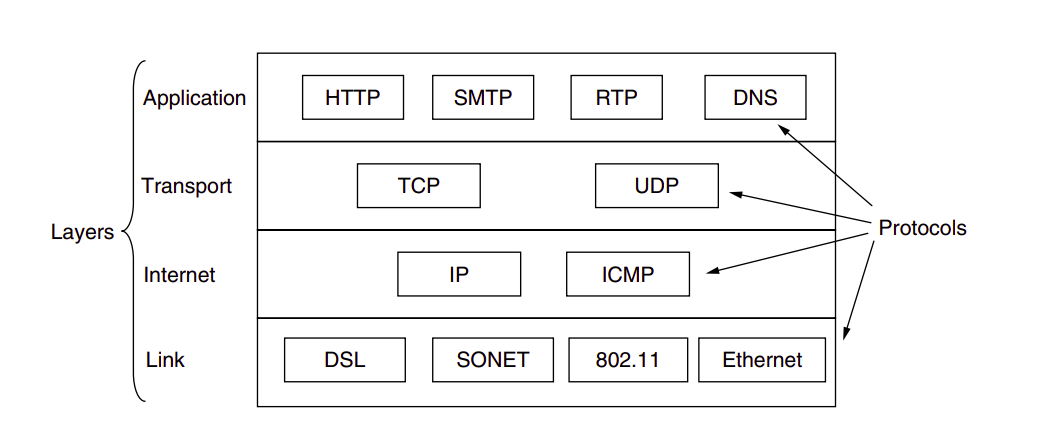
\includegraphics[width=100mm,height=50mm]{Slike/svi_protokoli.png}
                \end{center}
            \end{figure}
        \subsubsection{TCP/IP ili OSI model}
            \noindent \textbf{Zašto se OSI model ne koristi?}
            \begin{itemize}
                \item Loš tajming za investicije.
                \item Loša tehnologija (sloj sesije i prezentacije su skoro prazni).
                \item Loša implementacija.
                \item Loša politika.
            \end{itemize}
            Model Osi je svakako doprineo u razvoju mreža.\\

            \textbf{Mane TSP/IP sloja:}
            \begin{itemize}
                \item Nije dobar za izradu novih tehnologija, jer ne razlikuje koncepte
                      servisa, interfejsa i protokola.
                \item Loš za definisanje stek protokola (primer. nemoguće je definisati stek protokola 
                      za bluetooth)
                \item Ne postoji razlika između fizičkog sloja i sloja veze podataka.
            \end{itemize}
            \textbf{Model TCP/IP se koristi u praksi.}
            
    \subsection{jedinice podataka}
        \begin{itemize}
            \item Aplikativni - poruka
            \item Transportni - segment
            \item Mrežni - paket
            \item Sloj veze - okvir
            \item Fizički - bit
        \end{itemize}
        \subsection{orgranizacije za standarde}
        \begin{figure}[H]
            \begin{center}
                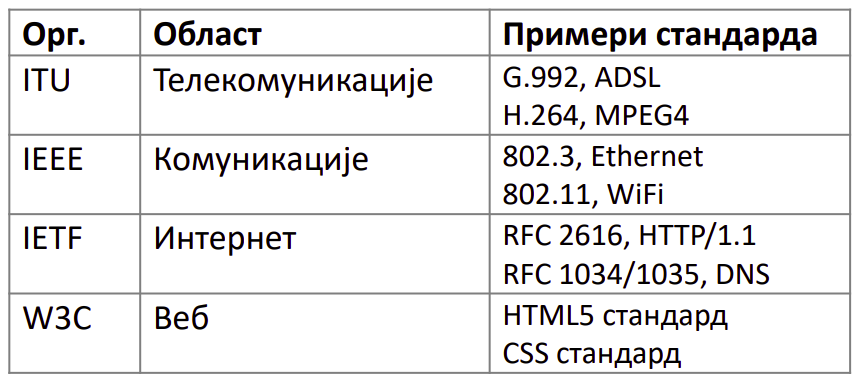
\includegraphics[width=100mm,height=50mm]{Slike/std_table.png}
            \end{center}
        \end{figure}

\section{Fizički sloj: uloga, pojednostavljeni model, kašnjenja, BDP, primeri. }
    \subsection{uloga}
        Podaci koji se prenose su digitalni (bitovi). Žice prenose analogni (fizički) signal. Ovo je 
        upravo uloga fizičkog sloja tj. fizički sloj šalje poruke putem komukacionog kanala. 
    \subsection{pojednostavljeni model}
        \textbf{Karakteristike:}
        \begin{itemize}
            \item Protok: brzina prenosa podataka (b/s, bitova po sekundi).
            \item Kašnjenje: vreme potrebno da poruka stigne na ciljnu adresu (s, sekundi).
            \item Da li kanal emituje signal ili ne.
            \item Raspodela verovatnoća grešaka.
            \item \dots
        \end{itemize}
        \begin{figure}[H]
            \begin{center}
                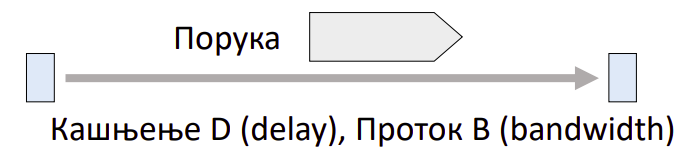
\includegraphics[width=80mm,height=25mm]{Slike/pojednostavljeni_fizicki.png}
            \end{center}
        \end{figure}
    \subsection{Kašnjenje}
        \textbf{Kašnjenje} predstavlja vreme potrebno da poruka stigne na ciljnu adresu. Merna jedinica
        za kašnjenje je sekunda (najćešće se koristi milisekunda). Sastoji se iz dva dela:
        \begin{itemize}
            \item \textbf{Kašnjenje prenosa (Transmission Delay):} Vreme potrebno da se M-bitovna poruka
                  postavi na komukacioni kanal:\\
                  T-delay = M (b) / B (b/s) = M/B (s), gde je B brzina postavljanja podataka na
                  komunikacioni kanal.
            \item \textbf{Kašnjenje propagacije (Propagation Delay):} Vreme potrebno da bitovi prođu 
                  kroz komukacioni kanal:\\
                  P-delay = dužina kanala/brzina signala ($\frac{2}{3}c)$ = X (s)
            \item Ukupno kašnjenje: \\
                  L = T + P = M/B + P
        \end{itemize}
    \subsection{BDP}
        Količina podataka prisutnih na kanalu u nekom momentu je \textbf{BDP (Bandwidth-Delay Product) tj. 
        proizvod protoka i kašnjenja}.
        Ako se podatak posmatra kao materija, onda bi ovo bila zapremina (količina) materije:\\
        \indent BDP = $B \cdot D$\\
        Vrednost BDP-a je mala za lokalne mreže, a velika za velike ,,debele mreže``.

    \subsection{Primeri (kašnjenje i BDP)}
        \noindent Primer kašnjenja: P = 5 ms, B = 56 Kb/s, M = 1250 B\\
        => P = 5/1000 s, B = 56*1024 b/s, M = 1250*8 b\\
        => L = 0.005 s + 1250*8 b / 56*1024 b/s\\
        => L = 0.005 s + 0.174 s\\
        => L = 0.179 s\\
        => L = 179 ms\\

        \noindent Primer BDP-a: B = 40 Mb/s, D = 50ms\\
        => B = 1024*1024*40 b/s, D = 0.05 s\\
        => BDP = 1024*1024*40 b/s * 0.05 s\\
        => BDP = 2097152 b\\
        => BDP = 262144 B\\
        => BDP = 256 KB\\
        => BDP = 0.25 MB\\
        Ovo se smatra visokim BDP-om.

\section{Žičani i optički komunikacioni medijumi}
    \subsection{UTP kablovi}
        \textbf{Upredene parice (UTP - Unshielded Twisted Pair)} su 
        veoma čest tip kanala. Sastoji se iz četiri upredene parice napravljene od bakra. Uvrtanjem
        bakarnih kablova se smanjuje smetnja. Koristi se u telekomunikacija i za ADSL internet pristup.
        Danas se koristi peta kategorija. Brzina prenosa je do 1 Gbps (full duplex). Parice su 
        osetljive na elektromagnetne smetnje. 
    \subsection{Koaksijalni kablovi}
        \textbf{Koaksijalni kablovi (Coaxial Cable)} su bolji komunikacioni medijum od upredenih
        parica po boljim performansama i manjim smetnjama, ali teži za održavanje. 
        Sastoji se od bakra u sredini, preko kojeg ide
        izolator, pa preko kojeg opet ide bakar ili aluminijum i spolja je obavijen 
        dodatnom izolacijom. Uglavnom idu uz kablovsku.
    \subsection{Instalacija za prenos struje}
        Već postoje u okviru naših kuća, ali imaju loše performanse.
    \subsection{Optički kabal}
        \textbf{Optički kablovi (Fiber-Optic Cable)} se prave od dugačkih, tankih i čistih vlakni stakla. 
        Imaju ogroman protok zbog opsega frekvencije i predstavljaju odličan komunikacioni medijum 
        za velike udaljenosti zbog malog slabljenja signala. Postoje dve vrste: \underline{višemodalno}
        (za manje udaljenosti) i \underline{unimodalno} (za veće udaljenosti). Prednosti staklenih vlakana u 
        odnosu na bakar su: bolje performanse, manja osetljivost na elektromagnetne smetnje 
        i bolji signal na većim udaljenostima.

\section{Bežični komunikacioni medijumi}
        Prednost i mana bežičnog prenosa je što se signal šalje u svim pravcima. To znači da može da
        ima više primaoca, ali signali sličnih frekvencija mogu da se mešaju i samim tim oštećuju.\\
        \subsection{Radio talasi}
        \textbf{Radio talasi (Radio Waves)} se lako generišu, mogu da putuju daleko i prolaze kroz zidove. Na malim 
        frekvencijama (VLF - Very Low Frequency, LF - Low Frequency, MF - Medium Frequency) talasi prate zakrivljenost 
        Zemlje, dok na velikim frekvencijama se odbijaju od jonosfere.
        \begin{figure}[H]
            \begin{center}
                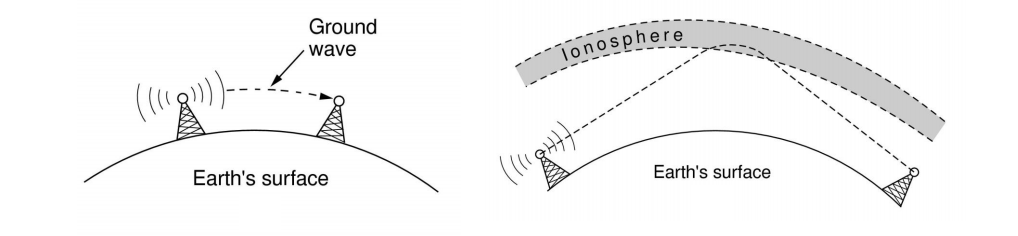
\includegraphics[width=125mm,height=50mm]{Slike/radio_talasi.png}
            \end{center}
        \end{figure}
        \subsection{Mikrotalasi}
        \textbf{Mikrotalasi (Microwaves)} imaju veliki frekventni opseg i koriste se često za zatvorene namene
        poput wifi, kao i za otvorene poput 3G i sateliti. Signal mikrotalasa slabi i reflektuje
        se od objekata okruženja. Jačina varira od udaljenosti, sabiranja signala, itd\dots
        \subsection{svetlost}
        Svetlost kao talas se može koristiti kao komunikacioni medijum, ali to je više za hrabre
        koji vole avanture.
        \subsection{Žičani i bežični prenos}
        \noindent \textbf{Prednost bežičnih u odnosu na žičane kanale:}
        \begin{itemize}
            \item Jednostavne i jeftine;
            \item Prirodno podržavaju mobilnost;
            \item Prirodno podržavaju emitovanje.
        \end{itemize}
        \textbf{Mane bežičnih u odnosu na žičane kanale:}
        \begin{itemize}
            \item Mešanje signala se mora razrešiti;
            \item Jačina signala (samim tim i protok) jako variraju.
        \end{itemize}
        \textbf{Prednost žičanih u odnosu na bežične kanale:}
        \begin{itemize}
            \item Lako se projektuje fiksni protok duž odabranih ruta.
        \end{itemize}
        \textbf{Mane žičanih u odnosu na bežične kanale:}
        \begin{itemize}
            \item Skupo za postavljanje, posebno na većim udaljenostima;
            \item Nisu projektovani za mobilnost i emitovanje.
        \end{itemize}

\section{Komunikacioni sateliti}
        Sateliti su efikasni za emitovanje i komunikaciju ,,bilo kad, bilo gde``. Osnovna podela
        satelita je po udaljenosti od zemlje gde razlikujemo \textbf{LEO (Low Earth Orbit)}, 
        \textbf{MEO (Medium Earth Orbit)} i \textbf{GEO (Geostationary orbit)} satelite. Postoje
        pojasevi Zemljine atmosfere gde ne mogu biti postavljeni sateliti. Ti pojasevi se nazivaju
        \textit{Van Alen pojasevi} i svaki satelit koji se tu postavi biva brzo uništen od strane čestica.
        Postoje dva takva pojasa i nalaze se između LEO i MEO, MEO i GEO što je jedan od 
        razloga za ovakvu podelu.
        \begin{figure}[H]
            \begin{center}
                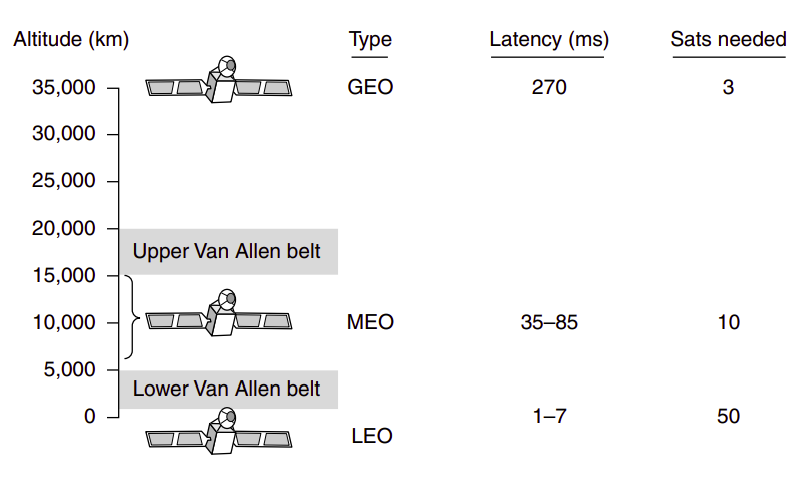
\includegraphics[width=90mm,height=70mm]{Slike/sateliti.png}
            \end{center}
        \end{figure}
        \subsection{Geostacionarni sateliti (GEO)}
            Ovi sateliti orbitiraju 35km iznad fiksne lokacije. Mikrostanice VSAT (Very Small 
            Aperture Terminals) dobijaju i šalju signal ka centralnoj stanici HUB koja služi 
            za komunikaciju između VSAT mikrostanica. Signali se šalju uz pomoć GEO satelita.
            Primer: emitovanje televizijskog programa.
            \begin{figure}[H]
                \begin{center}
                    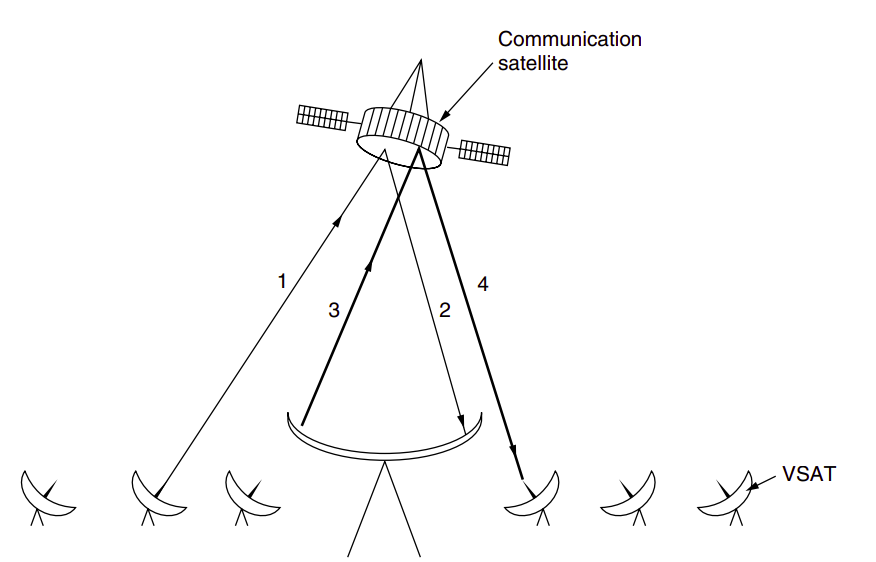
\includegraphics[width=90mm,height=70mm]{Slike/geo.png}
                \end{center}
            \end{figure}
        \subsection{Srednje visoko-orbitni sateliti (MEO)}
            Postavljeni su između dva Van Alen pojasa i koriste se uglavnom za GPS
        \subsection{Nisko-orbitni sateliti (LEO)}
            Zbog velike brzine potreban je veliki broj ovakvih satelita za kompletan sistem. Ovi 
            sateliti imaju manje kašnjenje zbog male udaljenosti od zemlje. Projekat koji je pokrenuo
            masovno korišćenje ovih satelita je \textit{Iridium} (77 satelita i 77 element u tablica, a
            zapravo je na kraju poslato 66 satelita). \\
            \indent Postavljeni su kao 6 lanaca oko planete. Imaju brži odziv od GEO satelita.
            \begin{figure}[H]
                \begin{center}
                    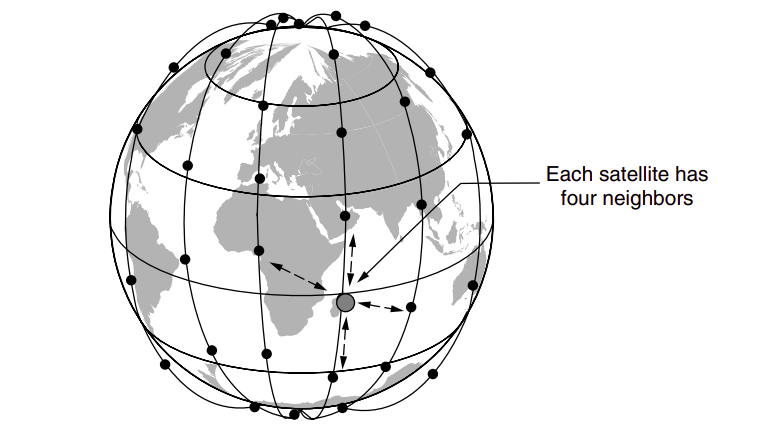
\includegraphics[width=100mm,height=60mm]{Slike/leo.png}
                \end{center}
            \end{figure}
        \subsection{Sateliti i optika}
            \noindent \textbf{Prednosti satelita u odnosu na optiku:}
            \begin{itemize}
                \item Nakon uspostavljenog kompletnog sistema se može komunicirati bilo gde;
                \item Emitovanje na velika područja;
                \item Instalacija nije skupa i komplikovana kao kod optike.
            \end{itemize}
            \textbf{Prednosti optike u odnosu na satelite:}
            \begin{itemize}
                \item Sateliti imaju ograničen protok i mešaju se signali;
                \item Ogroman protok duž velikih udaljenosti.
            \end{itemize}

\section{Signali: prenos, frekvenciona reprezentacija, signal u žičanim, optičkim, bežičnim medijumima.}
    \subsection{Prenos - Furijeova analiza}
        Svaka periodična funkcija g(t) može da se predstavi kao beskonačna suma sinusa i kosinusa:
        \begin{figure}[H]
            \begin{center}
                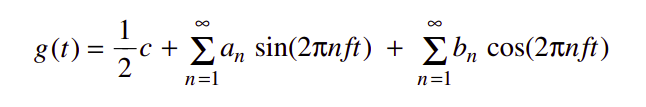
\includegraphics[width=125mm,height=20mm]{Slike/furije1.png}
            \end{center}
        \end{figure}
        Vrednosti $a_n$ u $b_n$ su sinusna i kosinusna amplituda n-te harmonijske težine, 
        i mogu se lako izračunati (kao i konstanta c). Takođe iz Furijeovog reda je 
        moguće rekonstruisati nazad funkciju. Pošto su svi podaci konačni, možemo ih 
        posmatrati kao da su periodični što je dovoljan uslov za Furijeovu transformaciju. 
        Sa desne strane su prikazane vrednosti $\sqrt{a_n^2 + b_n^2}$:
        \begin{figure}[H]
            \begin{center}
                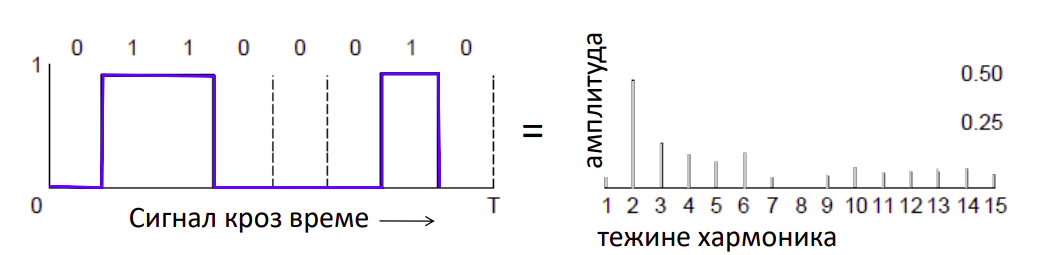
\includegraphics[width=125mm,height=40mm]{Slike/furije2.png}
            \end{center}
        \end{figure}
        
        U praksi ne možemo uzeti beskonačno frekvencija. Dovoljno je uzeti broj frekvencija
        tako da može da se rekonstruiše funkcija. Sa slike(dole) se vidi da pod (e) je dovoljno
        precizno i nije potreban veći broj frekvencija (manji skup frekvencija = manji protok):
        \begin{figure}[H]
            \begin{center}
                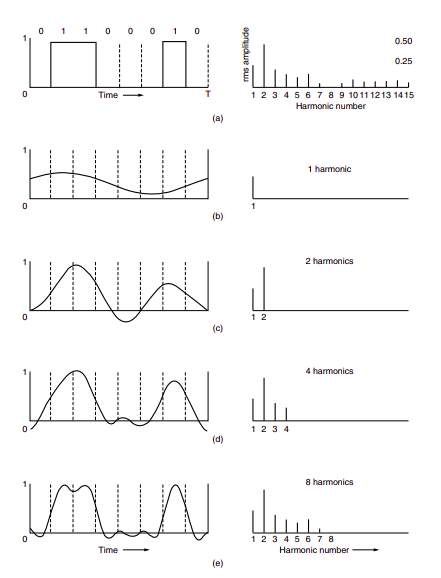
\includegraphics[width=120mm,height=120mm]{Slike/furije3.png}
            \end{center}
        \end{figure}
    \subsection{Prenos preko žice}
        \noindent \textbf{Šta se dešava sve sa signalom dok prolazi kroz žicu?}
        \begin{itemize}
            \item Signal kasni (brzina je $\frac{2}{3}c$, nije beskonačna);
            \item Signal slabi (srazmerno udaljenosti)
            \item Frekvencije iznad neke granice brže slabe;
            \item Dešava se šum (zbog spoljašnjih efekata).
        \end{itemize}
    \subsection{Prenos preko svetlosti}
        Svetlost se prenosi sa veoma malim gubitkom u tri široka frekvetna opsega.\\
        
    \subsection{Prenos preko bežičnih medijuma}
        Zbog velikih frekvencija bežičnih prenosa, nije moguće digitalni signal direktno kodirati
        u analogni, već se koristi koncept \textbf{signala nosaša} (signal putuje jako brzo, ali
        slabi sa kvadratom rastojanja). Takođe, problem kod bežičnih komunikacije to što se signali
        mešaju (ako su dovoljno blizu). Dodatni otežavajući efekti su to što je propagacije bežičnog
        signala složena i zavisi od okruženja, i karakteristike zavise od frekvencije (primer: problem
        sa sabiranjem odbijenih talasa). Signali mogu da se odbijaju od objekata i putuju kroz više 
        nezavisnih putanja. Kada signali stignu do primaoca oni mogu da budu pogrešno sabrani.

\section{Modulacija i multipleksiranje signala. }
    \subsection{Modulacija}
        Modulacija je način predstavljenja digitalnih informacija u okviru fizičkog medijuma.
        \subsubsection{Direktna modulacija (baseband)}
        Primer jednostavne šeme je \textbf{NRZ (Non-Return to Zero) šema}, gde visoki napon (+V) predstavlja 1, 
        a niski napon (-V) predstavlja 0. Može se koristiti više od dva nivoa (primer: prenosi se po
        2 bita). To zavisi od tehnoloških mogućnosti medijuma.\\

        
        \textbf{Problem kod dekodiranja: } Prilikom dekodiranja časovnici nisu toliko precizni u slučaju 
        dugih jedinica i nula. Niz 15 nula dosta liči na niz 16 nula osim ako časovnik 
        nije poprilično precizan.
        \begin{itemize}
            \item \textbf{Odvojeni kanal za časovnik:} Koriste se dupli kanali, gde se na drugom 
                  kanalu šalje signal časovnika.  
            \item \textbf{Mančester kodiranje:} Problem prethodnog rešenja je u tome što se 
                  bezveze koristi još jedan kanal,
                  gde on može da se koristi za prenos podataka. Bolje rešenje je da se pomeša 
                  signal časovnika sa signalom podataka koristeći XOR operator. Ovo kodiranje 
                  se naziva Mančester kodiranje.
                  (\href{https://www.youtube.com/watch?v=XKtxxZ327UM}{Manchester Encoding})
            \item \textbf{NRZI (Non-Return to Zero Inverted):} Kodiramo 1 kao prelaz 
                  ($1 \rightarrow 0, 0 \rightarrow 1$), 
                  a 0 kao neprelaz ($0 \rightarrow 0, 1 \rightarrow 1$). 
                  standard za USB koristi ovakav način kodiranja. Ovom metodom se samo rešava problem uzastopnih
                  jedinica, ali ne i uzastopnih nula.
            \item \textbf{4B/5B: } Svaki niz četiri bita se preslikava u niz 5 bitova. Preslikavanje
                  se bira tako da nikad nema više od tri uzastopne nule. Ovim se koristi 25\% više
                  bitova da se prenese poruka (i dalje bolje od Mančestera koji tehnički koristi 100\%
                  više). 
            \item \textbf{Scrambling: } Generiše se pseudo nasumični broj i XOR-uje se sa podacima u
                  nadi da neće da se desi niz dugačkih nula. 
        \end{itemize}
        \begin{figure}[H]
            \begin{center}
                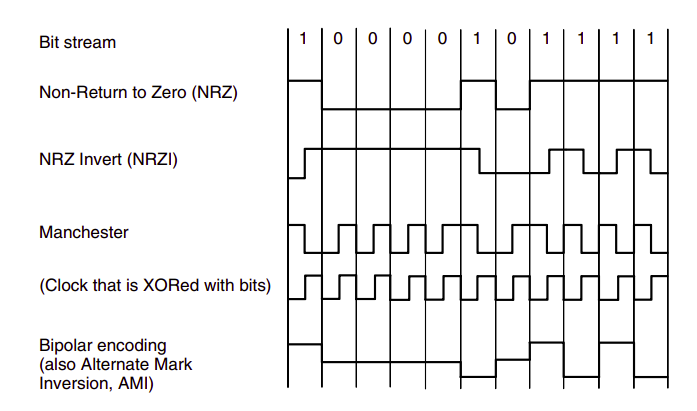
\includegraphics[width=120mm,height=60mm]{Slike/kodiranje1.png}
            \end{center}
        \end{figure}

        
        \subsubsection{Modulacija preko nosača (passband)}
            Direktna modulacija je moguća samo kod žičanih komunikacionih kanala. Kod bežičnih signala
            se koristi modulacija preko nosača, gde se signal kodira indirektno. Signal nosač oscilira
            na na željenoj frekvenciji, a potom se modulira promenom amplitude, frekvencije ili faze.
            \begin{itemize}
                \item \textbf{ASK (Amplitude Shift Keying)} - dve različite amplitude se koriste za reprezentaciju
                      nule i jedinice.
                \item \textbf{FSK (Frequencey Shift Keying)} - slično, koriste se različite frekvencije.
                \item \textbf{PSK (Phase Shift Keying)} - slično, koriste se različite faze.
                \item Takođe se može se koristiti kombinacije ASK, FSK i PSK.
            \end{itemize}
            \begin{figure}[H]
                \begin{center}
                    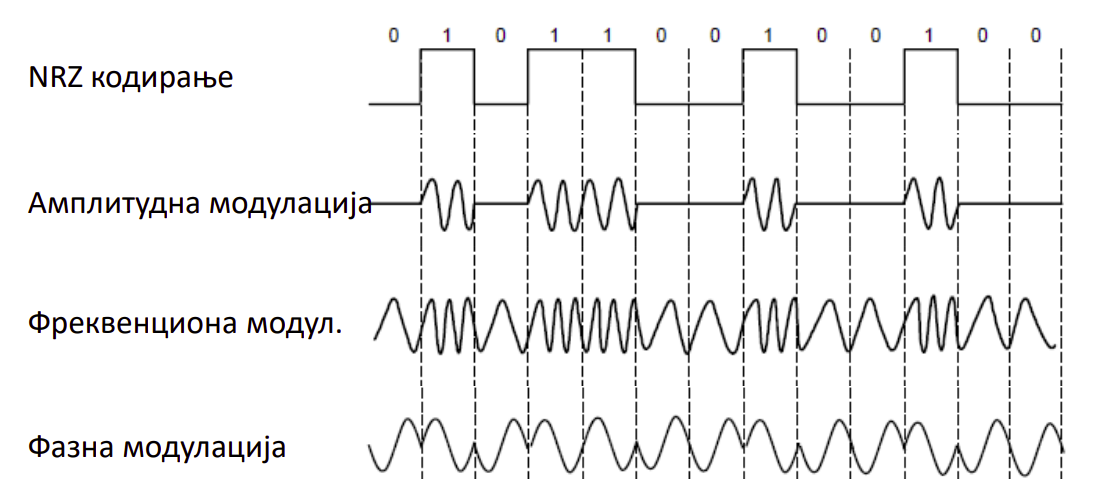
\includegraphics[width=120mm,height=60mm]{Slike/kodiranje2.png}
                \end{center}
            \end{figure}
            \textbf{Kombinovana amplitudno-fazna modulacija(QAM-16):}
            \begin{figure}[H]
                \begin{center}
                    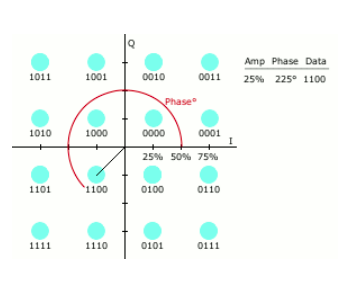
\includegraphics[width=80mm,height=60mm]{Slike/kodiranje3.png}
                \end{center}
            \end{figure}
            \underline{Ostale kombinacije:}
            \begin{itemize}
                \item BPSK: variranje faze, dve faze (jedan bit).
                \item QPSK: varivanje faze, četiri faze (dva bita)
                \item QAM-64: slično kao QAM-16, ali kodira 6 bitova.
            \end{itemize}
            \begin{figure}[H]
                \begin{center}
                    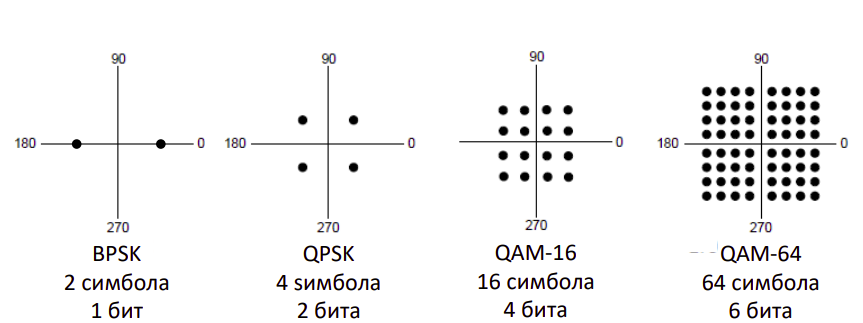
\includegraphics[width=120mm,height=45mm]{Slike/modulacija_preko_nosaca_primeri.png}
                \end{center}
            \end{figure}

    \subsection{Multipleksiranje signala}
        Multipleksiranje se bavi deljenjem kanala između više korisnika. Analogan iz života problem:
        U sobi ima puno ljudi koji trebaju međusobno da komuniciraju:
        \begin{itemize}
            \item \textbf{FDM (Frequency Division Multiplexing):} Korisnici kanala su postavljeni na 
                  različite frekvencije. U sobi punoj ljudi ovo bi bilo analogno da se ljudi
                  fokusiraju na ljude koji pričaju glasno, srednje ili slabo.
                  \begin{figure}[H]
                    \begin{center}
                        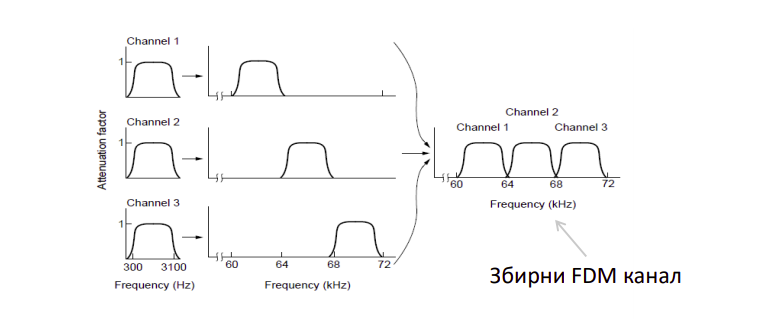
\includegraphics[width=100mm,height=40mm]{Slike/fdm.png}
                    \end{center}
                  \end{figure}
            \item \textbf{TDM (Time Division Multiplexing):} Kanal se deli vremenski, gde se korisnici
                  drže fiksnog rasporeda (upotrebljava se u sistemima fiksne telefonije). U sobi punoj 
                  ljudi ovo bi značilo da svi ćute dok drugi priča. Primer prioriteta: Round robin.
                  \begin{figure}[H]
                    \begin{center}
                        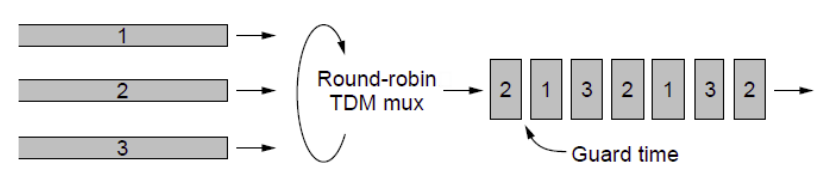
\includegraphics[width=100mm,height=30mm]{Slike/round_robin.png}
                    \end{center}
                  \end{figure}
            \item \textbf{CDMA (Code Division Multiple Access):} Korisnicima se dodeljuju ključevi.
                  Ključevi su međusobno ortogonalni. Na ortogonalni signal se primenjuje ključ (skalarni
                  proizvod). U sobi punoj ljudi ovo bi značilo da ljudi pričaju različitim jezicima.
                  \begin{figure}[H]
                    \begin{center}
                        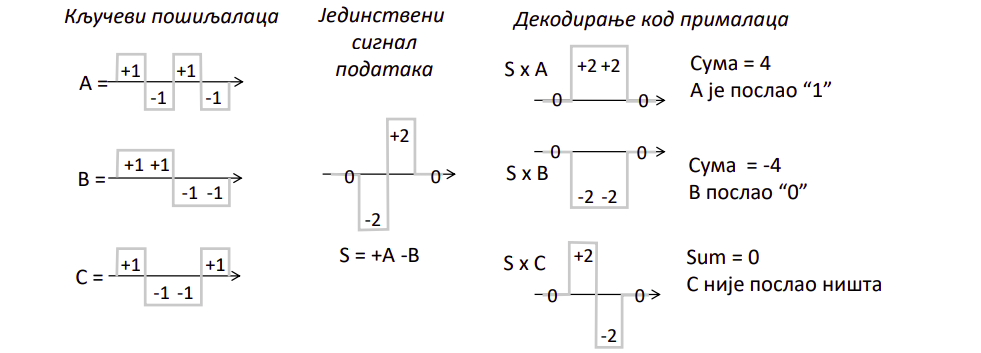
\includegraphics[width=120mm,height=40mm]{Slike/multipleksiranje.png}
                    \end{center}
                  \end{figure}
        \end{itemize}

\section{Prirodna ograničenja prenosa signala.}
    \textbf{Kako odrediti da li je prenos signala dobar?} \\
    Ako brzina prenosa signala blizu prirodnog ograničenja, onda je sistem dobro realizovan. Pojmovi:
    \begin{itemize}
        \item \textbf{B (Bandwidth, protok)} - ograničava brzinu promena (karakteristika kanala);
        \item \textbf{S (Signal power, jačina signala)} i \textbf{N (Noise power, jačina šuma)}. 
              Jačina šuma ograničava broj razlučivih nivoa signala (karakteristika primaoca).
              \textbf{Napomena:} Prilikom računanja limita i kapaciteta koriste prosečna jačina signala
              i prosečna jačina šuma.
    \end{itemize} 

    \textbf{Najkvistov limit:} Maksimalan broj promena je 2B. Ako postoji V nivoa signala, onda je
    maksimalan protok u bitovima: $R = 2B\cdot \log_2{V}$. Za V=2 je to R = 2B. \textbf{Napomena:}
    Ovo važi za kanale bez šuma.\\

    \textbf{Šenonov kapacitet:} Broj razlučivih nivoa signala zavisi od odnosa jačine signala i 
    jačine šuma $SNR = \frac{S}{N}$ \textbf{(SNR - Signal Noise Ratio, odnos šum-signal)}. 
    Vrednost SNR-a može jako da varira, zbog čega se on računa u decibilima tj. $SNR_{dB} = 10 \log_{10}{\frac{S}{N}}$. 
    Šenonov kapacitet je: $C = B\cdot \log_2{(1+\frac{S}{N})}$ b/s. Broj razlučivih signala se dobija 
    iz odnosa: $\frac{S+N}{N}=1+\frac{S}{N}$. \textbf{Napomena:} Da bismo duplirali Šenonov kapacitet nije
    dovoljno duplirati protok, jer je šum zavisan od protoka. \\
    \indent Kod žičanih komunikacija se može projektovati ciljni SNR i samim tim i ciljni prenos. Kod
    bežičnih SNR može drastično da varira za dato B (do 60db). Kod bežičnih komunikacija se mora
    ,,živeti`` na visokim varijacima. 

\section{Pregled relevatnijih sistema komunikacije.}
    \subsection{Sistem fiksne telefonije}
        \noindent Sistem fiksne telefonije (landline, fixed-line) se sastoji iz tri glavne komponente:
        \begin{itemize}
            \item \underline{Lokalne konekcije} (upredene parice koje idu do zgrada)
            \item \underline{Međumesne konekcije} (optički kablovi)
            \item \underline{Centrale} (gde se pozivi preusmeravaju)
        \end{itemize}
        Preko ovog sistema se realizuje DSL (ADSL).
    \subsection{Sistem mobilne telefonije}
        \noindent \textbf{Generacije:}
        \begin{itemize}
            \item \textbf{1G: analogni glas,} FM modulacija (kao kod radija), odvojena frekvencija 
                  za slanje i primanje 
            \item \textbf{2G: digitalni glas,} GSM (Global System for Mobile communication), 
                  QPSK modulacija
            \item \textbf{3G: digitalni glas i podaci,} UMTS (Universal Mobile Telecommunications System),
                  CDMA 
            \item \textbf{4G: digitalni glas i podaci,} LTE (Long Term Evolution), OFDM (napredni FDM)
        \end{itemize}
        \textbf{Organizacija baznih stanica:} Svaki mobilni korisnik koristi ćelijsku frekvenciju.
        Pri napuštanju jedne ćelije ulazi u drugu ćeliju (handoff). Iste frekvencije se mogu pronaći
        u nesusednim ćelijama. Za podržavanje većeg broja korisnika, obično se ograničava geografski
        prostor ćelije.
        \begin{figure}[H]
            \begin{center}
                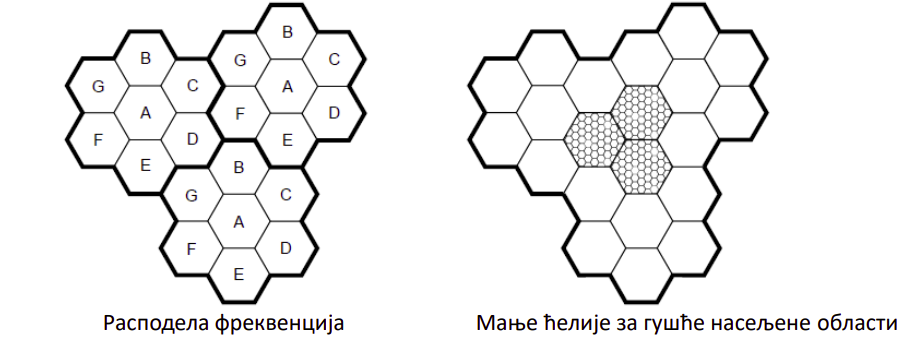
\includegraphics[width=120mm,height=50mm]{Slike/mobilne_celije.png}
            \end{center}
        \end{figure}
    \subsection{Internet preko kablovske}
        Internet kabl može da koristi već postojeću infrastrukturu za kablovsku televiziju.
        Drugačija je topologija u odnosu na telefonski sistem. Ovde ogranizacija podseća
        na topologiju magistrale. Preuzimanje i postavljanje podataka koriste opsege koji
        se ne koriste za gledanje TV programa.
    \subsection{Kablovska ili (A)DSL}
        \noindent \textbf{Prednosti kablovske:}
        \begin{enumerate}
            \item Koristi Koaksijalne kablove ka korisnicima koji imaju bolji protok od 
                  upredenih parica koje koristi ADSL.
        \end{enumerate}
        \textbf{Prednosti (A)DSL-a:}
        \begin{enumerate}
            \item Podaci se ne šalju svima kao kod kablovske, već posebnom koristniku.
            \item Protok nije deljen i ne varira toliko.
        \end{enumerate}
    

\section{Sloj veze: uloga, komunikacija sa slojem ispod i iznad, kratko objašnjenje spiska aktivnosti
na sloju veze. }
    Od fizičkog sloja imamo tok podataka (bitova). Želimo da šaljemo podatke kao celine tj. okvire
    fiksirane veličine koristeći mogućnosti fizičkog sloja. Poslovi sloja veze:
    \begin{itemize}
        \item Pruža dobro definisan intefejs mrežnog sloju;
        \item Proverava da li je došlo do greške tokom transmisije;
        \item Vodi računa o brzini protoka (ako je primalac sporiji od pošiljaoca).
    \end{itemize}
    \begin{figure}[H]
        \begin{center}
            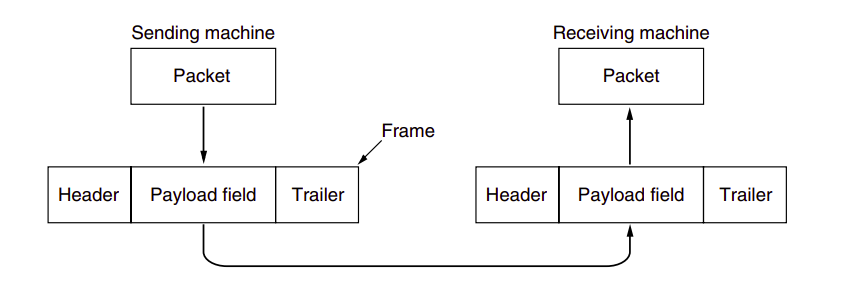
\includegraphics[width=120mm,height=50mm]{Slike/sloj_veze1.png}
        \end{center}
    \end{figure}

    \textbf{Servisi koje sloj veze nudi mrežnom sloju:}
    \begin{itemize}
        \item \textbf{Unacknowledged connectionless service: } Slanje nezavisnih okvira bez provere
              da li je stigao ispravan okvir do primaoca.
        \item \textbf{Acknowledged connectionless service: } Slanje nezavisnih okvira sa proverom
              da li je stigao ispravan okvir do primaoca.
        \item \textbf{Acknowledged connection-oriented service: } Uspostavlja se veza pre slanja niza
              okvira, gde se vodi računa za svaki okvir da li je stigao do primaoca.
    \end{itemize}

\section{Uokvirivanje u sloju veze}
    U teoriji uokvirivanje je potpuno nevidljivo fizičkom sloju. Ipak u praksi fizički sloj
    pomaže u identifikaciji okvira.\\
    
    \textbf{Brojanje bajtova:}  Okvir započinjemo sa poljem o njegovoj dužini. U slučaju greške na
    polju o njegovoj dužini dolazi do neusaglašavanja i ceo tok se poremeti.
    \begin{figure}[H]
        \begin{center}
            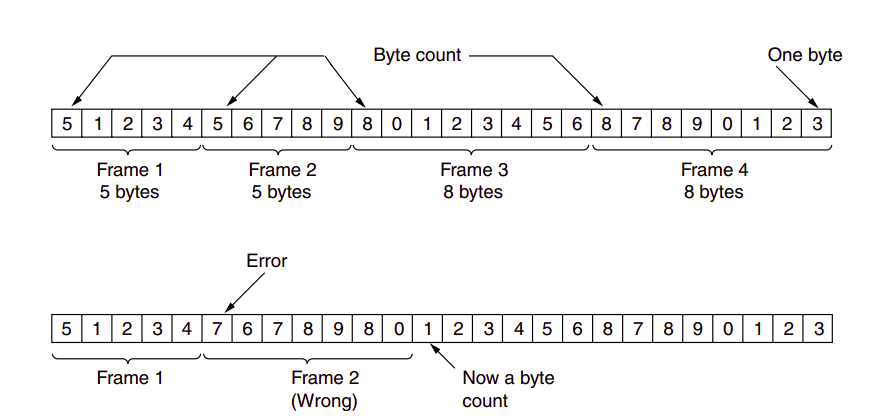
\includegraphics[width=120mm,height=50mm]{Slike/okvirivanje1.png}
        \end{center}
    \end{figure}

    \textbf{Umetanje bajtova:} Koristi se indikatorska oznaka, zastavica ,,FLAG`` u vidu bajta koja označava početak
    i kraj okvira. Potencijalni problem:
    \begin{itemize}
        \item \textbf{Šta ako se indikator nalazi u podacima?} Koristi se ,,ESC`` (escape) bajt sa leve
              strane ,,FLAG`` zastavice.
        \item \textbf{Šta ako se u podacima nalazi i ,,ESC``?} Opet, sa leve strane se doda ,,ESC``. 
              Prijemnik uvek usklanja prvi ,,ESC`` bajt, ako naiđe na ,,ESC`` bajt, i čita sledeći u nizu bajt.
              U slučaju da imaju dva ,,ESC`` za redom, onda bi pročitao tačno jedan. Ako naiđe na
              četiri uzaspona ,,ESC`` bajta, onda prijemnik čita tačno dva ,,ESC`` bajta.
    \end{itemize}
    \begin{figure}[H]
        \begin{center}
            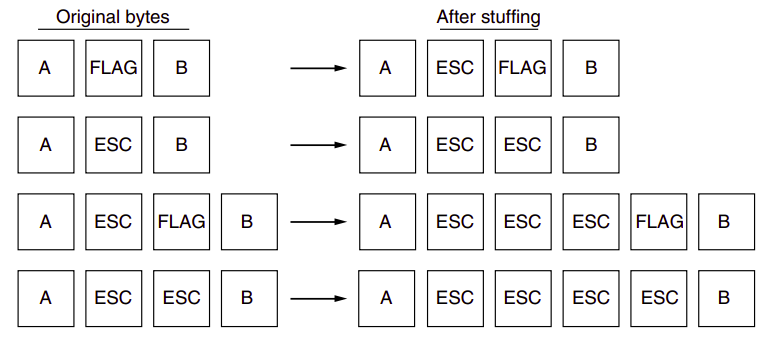
\includegraphics[width=120mm,height=50mm]{Slike/okvirivanje2.png}
        \end{center}
    \end{figure}
    \textbf{HDLC (High Level Link Control) protokol (umetanje bitova): } Početak i kraj okvira se 
    označavaju sa nizom bitova ,,01111110`` (zastavica). Ako se u podacima nalazi pet uzastopnih jedinica, 
    onda se nakon petog bita automatski ubaci jedna nula. U tom slučaju je nemoguće da se zastavica 
    nađe u podacima. Primalac, analogno, nakon svakih pet uzastopnih jedinica obriše jednu nulu.\\

    \noindent \underline{Poređenje metoda na podacima dužine 100 bajtova:}
    \begin{itemize}
        \item Bez zastavica se šalje 100 bajtova.
        \item Sa umetanjem bajtova u najgorem slučaju su sve specijalni bajtovi i šalje se 200 bajtova
              umesto 100 bajtove (do 100\% povećanja).
        \item Sa umetanjem bitova u najgorem slučaju je povećanje oko 12.5\%, jer se uz svaki bajt
              doda po jedan bit.
    \end{itemize} 
        
\section{Kodiranje grešaka u sloju veze.}
    Zbog sporednih efekata dolazi do šuma u signalu zbog čega nastaju greške u podacim. Postoje
    više načina za rešavanje ovakvog problema u zavisnosti od tipa šuma i njegove frekvencije.
    Postoje dva glavna pristupa: \underline{korekcija greške} i \underline{detekcija greške zajedno sa 
    retransmisijom.}
    Kod oba ova pristupa se dodaju redundantni podaci u okviru osnovnih podataka. Na osnovu
    redundantnih podataka se zaključuje da li je došlo do greške. Cilj je rešiti što više grešaka
    sa što manje redundantnosti.\\

    \textbf{Naivni pristup:} Poslati dve kopije za svaku poruku. Ako poruke nisu iste, onda je došlo
    do greške. Ovaj pristup može da detektuje grešku, međutim ako je došlo do greške ne možemo znati
    koja je kopija ispravna.\\

    U opštem slučaju kodna reč se sastoji iz D bitova podataka i R kontrolnih bitova. Proces:
    \begin{itemize}
        \item Pošiljalac izračuna R na osnovu D koristeći neku funkciju $f$ tj. R=$f$(D). 
        \item Pošiljalac šalje D+R bitova. 
        \item Primalac prihvata D+R bitova sa potencijalnim greškama. 
        \item Primalac računa R' na osnovu dobijenog D na isti način. 
        \item Ako se R i R' ne poklapaju, onda je došlo do greške.
    \end{itemize}

    \textbf{Intuicija:} Skup validnih kodnih reči je dosta manji od skupa mogućih reči. Slučajno
    odabrana reč ima malu šansu da bude ispravna. To znači da ako se desi greška, onda je mala
    šansa da će novodobijena reč biti validna.\\

\subsection{Hamingovo rastojanje} 
    \textbf{Hamingovo rastojanje} je minimalan broj inverzija koji je potreban
    da se od jedne validne reči dobije druga validna reč. Hamingovo rastojanje koda je minimalno Hamingovo
    rastojanje između parova validnih kodnih reči.
    \begin{itemize}
    \item \textbf{Detekcija grešaka:} Da bi se pouzdano otkrilo $d$ grešaka ($d$ izmenjenih bitova),
            Hamingovo rastojanje koda mora biti najmanje $d+1$. Tada je nemoguće da $d$ jednobitnih
            grešaka promene validnu kodnu reč u neku drugu validnu reč.
    \item \textbf{Korekcija grešaka:} Za kod sa Hamingovim rastojanjem $2d+1$, najviše $d$ grešaka
            se uvek može ispraviti do najbliže ispravne validne reči. Primer:
            \begin{itemize}
                \item Validne reči: 0000000000, 0000011111, 1111100000, 1111111111.
                \item Hamingovo rastojanje: 5, ($2\cdot2+1$) $=>$ može se napraviti bilo koja dvobitna 
                      greška.
                \item Primer: 0000000111 se ispravlja u 0000011111 ako je dvobitna greška,
                      ali ako je trobitna greška onda je možda 0000000000 poslata reč.
            \end{itemize}
    \end{itemize}

\section{Detekcija grešaka u sloju veze.}
    Na mrežama gde je šum manji kao što su optički kablovi ili bakar visokog kvaliteta, umesto
    korekcije kodova se više isplati detekcija uz retransmisiju. 

\subsection{Provera parnosti:} 
    Koristi se jedan dodatni bit za proveru parnosti. Ovaj bit
    se računa kao zbir podataka po modulu 2, odnosno XOR svih bitova u podacima. Ako se
    desi jednobitna greška onda se greška može detektovani. Ako se desi greška dva puta onda
    se greška ne može detektovati.
    \subsection{Kontrolni zbir: } Vrši se sumiranje podatak po kolonama (umesto po redovima).
    Ovaj metod se naziva \textbf{,,interleaving``} (računanje sume drugačijim redom od slanja podataka).
    Suma se dodaje kao poslednji red. Ova metoda ima bolju detekciju od provere parnosti.
    Kontrolna suma na \textbf{,,burst error``} (grupne greške, ekplozija grešaka):
    \begin{figure}[H]
    \begin{center}
        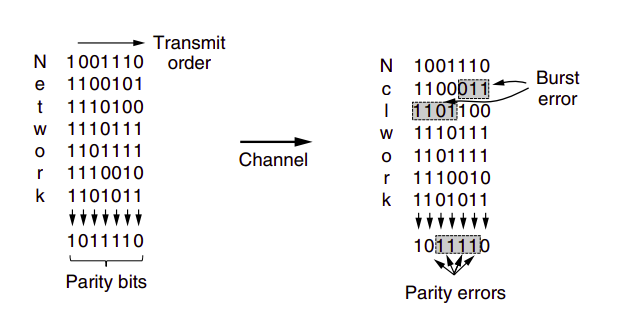
\includegraphics[width=120mm,height=60mm]{Slike/detekcija1.png}
    \end{center}
    \end{figure}

\subsection{Internet kontrolni zbir} 
    Bolja verzija kontrolnog zbira svodi se na korišćenje
    nepotpunog komplementa. Kontrolni zbir ima 16 bitova i predstavlja nepotpuni komplement
    sume reči po kolonama. Algoritam:
    \begin{itemize}
        \item Slanje:
            \begin{enumerate}
                \item Složiti podatke kao 16 bitne reči jednu ispod druge;
                \item Sabrati 16-bitne reči u nepotpunom komplementu;
                \item Negirati dobijenu sumu;
                \item Rezultat predstavlja kontrolnu sumu.
            \end{enumerate}
        \item Prihvatanje:
            \begin{enumerate}
                \item Složiti podatke kao 16 bitne reči jednu ispod druge;
                \item Sabrati 16-bitne reči u nepotpunom komplementu;
                \item Negirati dobijenu sumu;
                \item Nema greške ako je dobijeni rezltat 0, u suprotnom ima greške.
            \end{enumerate}
    \end{itemize}
    \begin{figure}[H]
    \begin{center}
        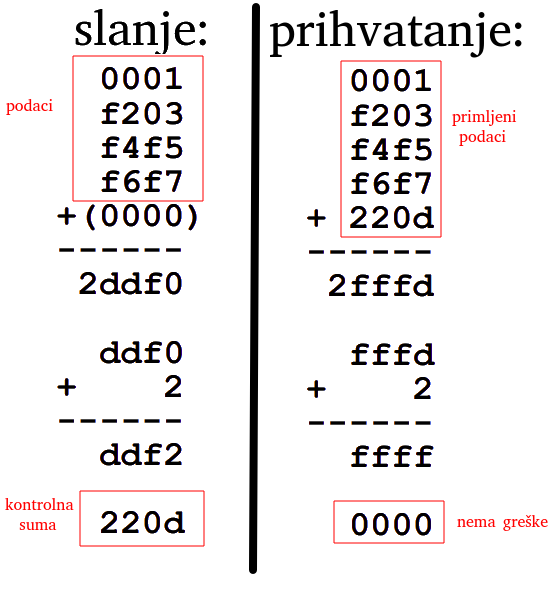
\includegraphics[width=60mm,height=60mm]{Slike/detekcija2.png}
    \end{center}
    \end{figure}

\subsection{Ciklična provera redundanse (CRC) ili polinomijalni kodovi} 
    Ideja je da se niz bitova tretira kao polinom sa koeficijentima 0 ili 1. Bitovski kod dužine k se
    posmatra kao polinom stepena k-1 tj. $b_0 + b_1 x + b_2 x^2 + ... + b_{k-1} x^{k-1}$, 
    gde je prvi bit (nulti bit) skroz desno u binarnom zapisu. Primer: 
    110001 odgovara polinomu $1x^5+1x^4+0x^3+0x^2+0x^1+1$. Sve aritmetičke operacije su po modulu 2 
    (sabiranje, oduzimanje, deljenje, množenje). \\
    \indent Potrebno je da se pošiljalac i primalac dogovore 
    oko generatora polinoma G(x). Ideja je da se doda k (dužina G(x)) bitova (CRC) na kraj tako da 
    polinom bude deljiv sa G(x) i da se pošalje novodobijeni kod. Primalac vrši deljenje dobijenog koda sa 
    G(x). Ako se dobije ostatak različit od nule, onda je došlo do greške. \underline{Algoritam:}
    \begin{enumerate}
        \item Neka je k dužina polinoma G(x). Dodaje se $k$ nula na kraj (desno) podatka D dužine n
              (dodavanje $k$ nula sa desne strane na bitovski zapis odgovara množenju polinoma sa $x^k$),
              kojem odgovara polinom $M(x)$. Novodobijeni kod je dužine $n+k$ i odgovara polinomu 
              $x^kM(x)$. 
        \item Izvrši se deljenje $x^kM(x)$ sa $G(x)$. Dobije se ostatak $R(x)$ dužine (najviše) $k$.
        \item Šalje se podatak koji odgovara polinomu $x^kM(x)+R(x)$ (doda se 
              polinom $R(x)$ sa desne strane $M(x)$) koji je deljiv sa $G(x)$.
    \end{enumerate}
    \begin{figure}[H]
        \begin{center}
            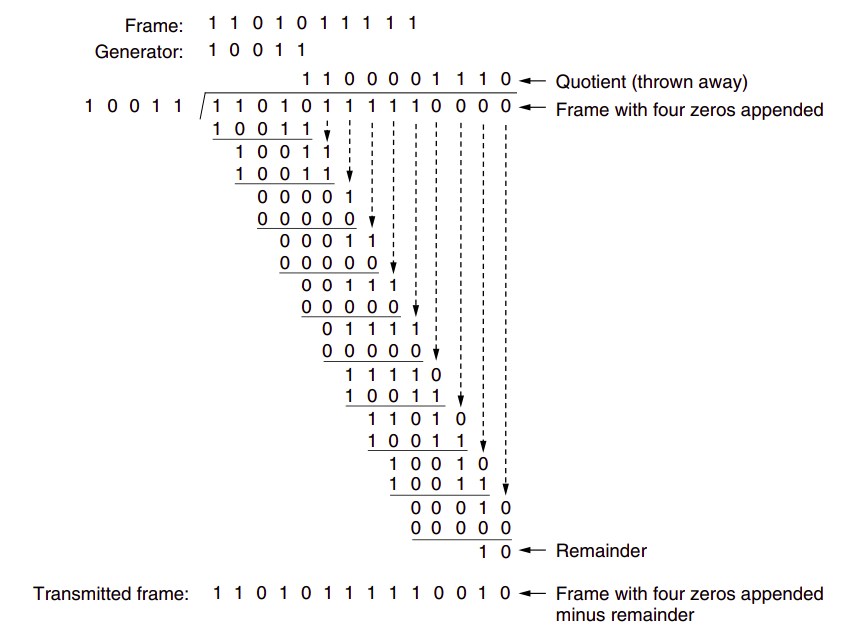
\includegraphics[width=120mm,height=80mm]{Slike/detekcija3.png}
        \end{center}
    \end{figure}

\subsection{Detekcija grešaka u praksi}
    Od generatora zavisi kvalitet CRC detekcije. Postoje standardni CRC-32 brojevi koji se koristi
    u praksi. Ciklična provera se koristi za Ethernet, 802.11, ADSL, kablovsku, \dots
    Kontrolni zbir (iako je lošiji) se koristi za protokole na višim slojevima kao što su IP, TCP,
    UDP, itd. Kontrola parnosti se slabo koristi.
    
\section{Korekcija grešaka u sloju veze}
    Korekcija greške se više primenjuje za bežičnu komunikaciju, gde je retransmisija skuplja i
    više se isplati pokušati sa izrvšavanjem korekcije.
    \subsection{Hamingov kod za korekciju HD=3}
        Koristi n bitova podataka i k kontrolnih bitova, gde važi veza $n = 2^k-k-1$ (primer. 
        $n=4$, $k=3$). Ideja je da se stavi kontrolni bit na pozicije koje su stepen dvojke (1, 2, 3,...).
        Kontrolni bitovi se i dalje uključuju kao bitovi za kontrolu parnosti uz bitove koji imaju
        vrednost (po indeksu) 1 na (i)-tom mestu. Primer ($n=4$, $k=3$): \\
        \indent 1: 001, 2: 010, 3: 011, 4: 100, 5: 101, 6: 110, 7: 111. \\
        \textit{Grupisanje}:
        \begin{itemize}
            \item Po bitu najmanje težine (desnom) tj. prvom bitu: 1, 3, 5 i 7;
            \item Po drugom bitu: 2, 3, 6, 7;
            \item Po trećem bitu se grupišu 4, 5, 6, 7. 
        \end{itemize}
        \begin{figure}[H]
            \begin{center}
                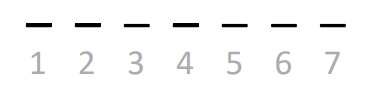
\includegraphics[width=30mm,height=14mm]{Slike/haming1.png}
            \end{center}
        \end{figure}
        Primer: Neka su podaci D = 0101 => tri kontrolna bita se koriste! Podaci za slanje su oblika:
        ? ? 0 ? 1 0 1, tj. $p_1 p_2 0 p_3 1 0 1$, gde su $p_1, p_2, p_3$ kontrolni bitovi parnosti. U
        opštem slučaju su podaci oblika: $p_1 p_2 d_1 p_3 d_2 d_3 d_4$, gde su $d_1, d_2, d_3, d_4$ 
        bitovi podataka.
        \begin{itemize}
            \item $p_1 = d_1\oplus d_2\oplus d_4 = 0\oplus1\oplus1 = 0$
            \item $p_2 = d_1\oplus d_3\oplus d_4 = 0\oplus0\oplus1 = 1$
            \item $p_3 = d_2\oplus d_3\oplus d_4 = 1\oplus0\oplus1 = 0$
        \end{itemize}
        \textit{Dodatno objašnjenje:} $d_1$ ima poziciju 3, $d_2$ poziciju 5, $d_4$ poziciju 7, a iz 
        prethodnog znamo da se bitovi na pozicijama 1, 3, 5, 7 (grupisanje po prvom bitu) koriste za kontrolu parnosti.
        Ovakvim biranjem vrednost $p_1$, $p_2$, $p_3$ odmah znamo da li su podaci koju su pristigli ispravni 
        ili ne ako njihova suma po modulu 2 nije 0 (primer: za dobijeni podatak $b_1 b_2 b_3
        b_4 b_5 b_6 b_7$ proveravamo da li je $b_1 \oplus b_3 \oplus b_5 \oplus b_7 = 0$). Tačnije, 
        $p_1$, $p_2$ i $p_3$ biramo tako da XOR grupa (iznad navedeno grupisanje) bude 0.\\
        \textit{Dekodiranje:}
        \begin{itemize}
            \item \textit{Prvi slučaj:} Pristigao kod je 0100101 ($b_1 b_2 b_3 b_4 b_5 b_6 b_7$). 
                  Proverava se parnost bitova p1, p2 i p3 (XOR):
                  \begin{itemize}
                      \item $p_1 = b_1 \oplus b_3 \oplus b_5 \oplus b_7 = 0\oplus 0\oplus 1\oplus 1 = 0$
                      \item $p_2 = b_2 \oplus b_3 \oplus b_6 \oplus b_7 = 1\oplus 0\oplus 0\oplus 1 = 0$  
                      \item $p_3 = b_4 \oplus b_5 \oplus b_6 \oplus b_7 = 0\oplus 1\oplus 0\oplus 1 = 0$
                  \end{itemize}
                  Rezultat je 000 => Nema greške! Podatak je 0101 ($b_3 b_5 b_6 b_7$, čitaju se svi bitove
                  čiji indeks nije stepen dvojke).
            \item \textit{Drugi slučaj:} Pristigao kod je 0100111 (greška na pretposlednjem bitu tj. šestom bitu). 
                  Proverava se parnost bitova $p_1$, $p_2$ i $p_3$:
                  \begin{itemize}
                      \item $p_1 = b_1 \oplus b_3 \oplus b_5 \oplus b_7 = 0\oplus 0\oplus 1\oplus 1 = 0$
                      \item $p_2 = b_2 \oplus b_3 \oplus b_6 \oplus b_7 = 1\oplus 0\oplus 1\oplus 1 = 1$  
                      \item $p_3 = b_4 \oplus b_5 \oplus b_6 \oplus b_7 = 0\oplus 1\oplus 1\oplus 1 = 1$
                  \end{itemize}
                  Rezultat (sindrom) je 110 ($p_3 p_2 p_1$, unazad) => Greška, bit na poziciji 110 (6) je
                  komplementiran. Ispravlja se greška i konačan podatak se čita iz 0100101. Konačan
                  rezultat je 0101. \textbf{Napomena:} Da su dva bita bila komplementirana ne bi se mogla ispraviti
                  greška, ali bi se mogla uočiti (detektovati).
        \end{itemize}
    
    \subsection{Kodovi za korekciju u praksi}
        \noindent U praksi se Hamingovi kodovi retko koriste. U upotrebi su najčešće:
        \begin{itemize}
            \item Konvolucioni algoritmi
            \item Metoda parnosti za malu gustinu
            \item Rid-Solomonovi kodovi
        \end{itemize}
    
    \subsection{Detekcija ili korekcija}
        Korekcija grešaka se koristi kada su greške očekivane ili kada nema vremena za retransimisju.
        Najčešće se koristi na fizičkom nivou. Detekcija grešaka je efikasna kada greške nisu očekivane
        tj. kada su retke. Koriste se na sloju veze u kombinaciji sa retransimisijom okvira.\\
        
        Primer: Neka je verovatnoća greške 0.001 (jednobitna greška na svakih 1000 bitova ili 
        100-bitna greška na svakih 100000 bitova). Neka je veličina okvira 100. Da li je bolja
        detekcija sa retransmisijom ili korekcija? Ako koristimo Hamingov kod sa $n=4$, $k=3$ (neki drugi
        je verovatno značajno efikasniji) onda na svakih 4 bita koristimo 7 bitova tj. na 100 bitova
        koristimo 175 bitova (75\% dodatnih bitova). Za jednobitne greške je ovo solidno rešenje (u 
        slučaju dvobitne greške izvršiti retransmisiju). Ako koristimo kontrolne sume sa dodatnih 16 bitova
        onda u proseku se svaki deseti okvir šalje duplo (na 10 potrebnih okvira se šalje 11 okvira).
        Deset okvira po 100 bitova (obični podaci) čini 1000 bitova. Jedanaest okvira po 116 bitova
        čini 1276 bitova (to je 27.6\% dodatnih bitova). Dodatno, ovom tehnikom se dedukuju i rafalne
        grešle. U ovom slučaju se verovatno isplati vršiti detekciju sa retransmisijom. 

\section{Sloj veze: tipovi servisa, okruženje, utopijski jednosmerni protokol.}
    \noindent \textbf{Servisi koje sloj veze nudi mrežnom sloju:}
    \begin{itemize}
        \item \textbf{Servis bez uspostavljene veze i bez potvrde prijema (Unacknowledged connectionless 
              service):} Slanje nezavisnih okvira bez provere da li je stigao ispravan okvir 
              do primaoca. Primer: Ethernet. 
        \item \textbf{Servis bez uspostavljene veze sa potvrdom prijema (Acknowledged connectionless 
              service):} Slanje nezavisnih okvira sa proverom da li je stigao ispravan okvir do 
              primaoca. Primer: Wifi.
        \item \textbf{Servis sa uspostavljenom vezom i potvrdom prijema (Acknowledged 
              connection-oriented service):} Uspostavlja se veza pre slanja niza
              okvira, gde se vodi računa za svaki okvir da li je stigao do primaoca.
              Retko se koristi.
    \end{itemize}

    \subsection{Okruženje: Pregled struktura i funkcija}
    Sloj veze je obično realizovan delom na mrežnoj kartici, a drugim delom na nivou operativnog
    sistema. \\

    Pregled nekih osnovih konstanti i struktura koji su potrebni za pseudokodove:
    \begin{lstlisting}
#define MAX PKT 1024                // determines packet size in bytes 
typedef enum {false, true} boolean; // boolean type 
typedef unsigned int seq nr;        // sequence or ack numbers 
typedef struct {
    unsigned 
    char data[MAX PKT];
} packet;                           // packet definition 
typedef enum {
    data, 
    ack, 
    nak
} frame kind;                       // frame kind definition 
typedef struct {                    // frames are transported in this layer 
    frame kind kind;                // what kind of frame is it? 
    seq nr seq;                     // sequence number 
    seq nr ack;                     // acknowledgement number 
    packet info;                    // the network layer packet 
} frame;\end{lstlisting}
    Pregled nekih funkcija za interakciju sloja veze sa slojem ispod i iznad:
    \begin{figure}[H]
        \begin{center}
            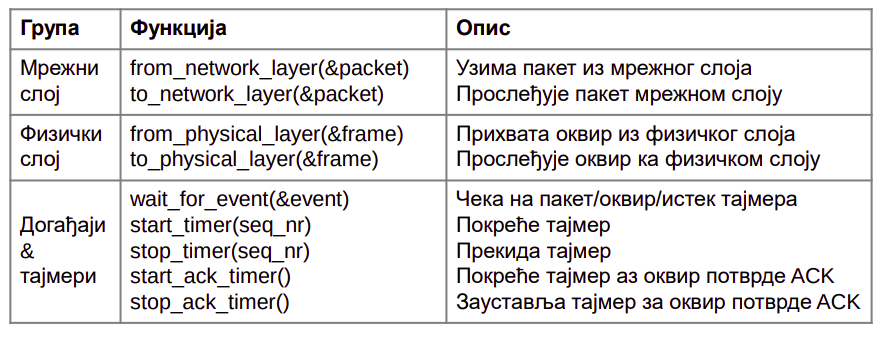
\includegraphics[width=120mm,height=45mm]{Slike/sloj_veze_funkcije.png}
        \end{center}
    \end{figure} 
    
    \newpage
    \subsection{Utopijski jednosmerni protokol}
        Utopijski jednosmerni protokol radi na sistemu u kojem se smatra da je vreme procesiranja nula,
        pošiljalac i primalac su uvek spremni da šalju i primaju podatke, okviri su otporni na greške,
        i okviri se ne gube tokom komunikacije. Zbog svoje savršenosti i nerealnosti se ovaj sistem naziva
        \textbf{,,Utopia``}. Protokol se sastoji iz dve procedure. Jedna procedura je za slanje, a druga
        za primanje podataka. Pseudokod za jednosmerni kanal:
  
\begin{lstlisting}
void sender()
{
    frame s;
    packet buffer;

    while(true)
    {
        from_network_layer(&buffer); // mrezni sloj prosledjuje paket
        s.info = buffer;             // paket se stavlja u okvir
        to_physical_layer(&s)        // okvir se prosledjuje za slanje
    }
}

void receiver()
{
    frame s;
    event_type event; // postoji samo jedan tip dogadjaja u ovom slucaju
    
    while(true)
    {
        wait_for_(&event);         // ceka se dogadjaj
        from_physical_layer(&s);   // uzima se okvir sa fizickog sloja
        to_network_layer(&s.info); // prosledjuje se paket na mrezni sloj
    }
}
\end{lstlisting}

    \newpage
\section{Kontrola toka, ARQ, pauze (tajmauti), duplikati, protokol „stani i čekaj“ za savršen i
nesavršen kanal. }

    \subsection{Protokol ,,Stani i čekaj`` za savršen kanal}
        Sada se pretpostavlja da pošiljalac i primalac ne moraju da imaju iste brzine slanja i primanja.
        U ovom slučaju je potrebna nekakva kontrola toka. Greške i dalje ne postoje. Jedno rešenje je
        da se napravi da primalac bude dovoljno brz da prihvati sve poruke bez problema. Ova metoda ne rešava
        problem, već ga samo odlaže. \\
        \indent \textbf{Protokol ,,stani i čekaj``} predstavlja jedno rešenje ovog problema. 
        Pošiljalac šalje jedan okvir i čeka da stigne \textbf{ACK (acknowledgement)} okvir od primaoca
        koji potvrđuje da je taj okvir stigao. Okvir ACK može da bude prazan. 
        Kada stigne ACK okvir, pošiljalac može da pošalje sledeći okvir. \textbf{Napomena:} Ovde je 
        dvosmerna komunikacija na kanalu, ali na se podaci šalju u jednom smeru. Pseudokod:

\begin{lstlisting}
void sender()
{
    frame s;
    packet buffer;
    event_type event; 

    while(true)
    {
        from_network_layer(&buffer);
        s.info = buffer;
        to_physical_layer(&s);
        wait_for_event(&event); // jedina razlika je sto se ovde ceka ACK
    }
}

void receiver()
{
    frame r, s; // r - receive, s - send
    event_type event; 
    
    while(true)
    {
        wait_for_event(&event);
        from_physical_layer(&r);
        to_network_layer(&r.info);
        to_physical_layer(&s); // jedina razlika sto se salje ACK
    }
}
\end{lstlisting} 

    \subsection{Protokol ,,Stani i čekaj`` za nesavršen kanal}
        Sada se dodatno pretpostavlja da se mogu desiti greške i okviri mogu biti izgubljeni.
        Problemi:
        \begin{itemize}
            \item Okvir može da se zagubi. Kako pošiljalac da zna da treba opet da ga pošalje?
            \item Ako primalac nekako javi pošiljaocu da se okvir zagubio, pošiljalac mu 
                  pošalje nov okvir, ali posle nekog vremena stigne i taj koji se zagubio.
                  Kako primalac da zna da treba da odbaci ovaj duplikat?
            \item Šta ako se ACK okvir izgubi?
        \end{itemize}
        Potreban je napredniji protokol. Rešenje ovog problema nudi \textbf{ARQ (Automatic Repeat reQuest)
        protokol}. Drugi naziv je \textbf{PAR (Positive Acknowledgement with Retransmission) protokol}.
        Nakon što se pošalje okvir uključuje se tajmer. Ako tajmer istekne, onda se okvir opet
        šalje. Potrebno je izabrati dobro vreme za brojac da ne bude dovoljno kratko ili dovoljno
        dugačko kako bi se povećale performanse sistema. Ako tajmer istekne, to znači da 
        se zagubio okvir koji je poslat ili se zagubio ACK okvir. Takođe se koristi serijski brojevi
        za okvire kako bi se oni razlikovali (kako bi znali da li stigao duplikat). Pošiljalac, dok traje 
        tajmer, može da očekuje tri slučaja:
        \begin{itemize}
            \item Stigao je ispravan ACK okvir;
            \item Stigao je neispravan ACK okvir ili ACK duplikat;
            \item tajmer je istekao.
        \end{itemize}
        Ako je stigao ispravan ACK okvir, onda se uzima sledeći paket sa mrežnog sloja, pomera se
        serijski broj za sledeći ACK okvir koji se očekuje i šalje se sledeći okvir (paket). U suprotnom 
        se šalje opet isti okvir. Slična stvar je i kod primaoca:
        \begin{itemize}
            \item Stigao je ispravan okvir;
            \item Stigao je neispravan okvir ili duplikat;
        \end{itemize}
        Ako je ispravan okvir, on se prosleđuje mrežnom sloju, šalje se ACK okvir primaocu 
        i pomera se serijski broj za sledeći okvir koji se čeka. U suprotnom (neispravan okvir ili 
        duplikat) se šalje opet ACK za poslednji ispravan okvir. Pseudokod:

\newpage
\begin{lstlisting}
void sender()
{
    seq_nr next_frame_to_send;
    frame s;
    packet buffer;
    event_type event;
    
    next_frame_to_send = 0;
    from_network_layer(&buffer);
    while(true)
    {
        s.info = buffer;
        s.seq = next_frame_to_send;
        to_physical_layer(&s);     // salje se okvir 
        start_timer(s.seq);        // i aktivira se brojac za odg. ser. broj
        wait_for_event(&event);   
        if(event == frame_arrival) // stigao je novi okvir
        {
            from_physical_layer(&s);
            if(s.ack == next_frame_to_send) // da li je ispravan broj okvira?
            {
                stop(s.ack); // prekida se brojac za odg. ser. broj
                from_network_layer(&buffer); // uzima se sledeci paket za slanje
                inc(next_frame_to_send);     // pomera se ser. broj
            }
        }
    }
}

void receiver()
{
    seq_nr expected_frame;
    frame r, s;
    event_type event;

    frame expected = 0;
    while(true)
    {
        wait_for_event(&event);
        if(event == frame_arrival) // stigao je okvir
        {
            from_physical_layer(&r);
            if(r.seq == expected_frame) // da li je ispravan broj okvira?
            {
                to_network_layer(&r.info);
                inc(frame_expected);
            }
            s.ack = 1 - expected_frame; // priprema se potvrda
            to_physical_layer(&s);      // i salje se primaocu
        }
    }
}
\end{lstlisting} 

\section{Protokol kliznih prozora u sloju veze, „1-bitni“, „vrati se N“, „selektivno ponavljanje“. }

    \subsection{Metoda ,,piggybacking``}
        Prethodni protokoli su prenosili okvire samo u jednom smeru, gde pošiljalac šalje 
        okvir primaocu i onda primalac šalje prazan ACK okvir nazad. U slučaju dvosmerne komunikacije
        bi bio potreban dupli simpleks kanal za dvosmernu komunikaciju. Bolja ideja je da se
        koristi metoda \textbf{,,šlepanje`` (,,piggybacking``)}. Ova metoda podrazumeva da umesto da se odmah šalje
        prazan ACK okvir za potvrdu, sačeka (neko vreme) da se spremi okvir koji bi svakako trebalo da bude
        poslat i zakači ACK broj na njega. Koristeći ovu metodu ostvaruje se mogućnost dvosmerne
        komunikacije koristeći jedan kanal. Međutim, ovo stvara nove probleme. \\
        \indent Neka postoje dva čvora u komunikacija na jednom kanalu tj. prvi čvor i drugi čvor.
        Oba čvora mogu da šalju i primaju okvire. Primenjuje se ,,piggybacking``. Situacija je sledeća:
        Prvi čvor je poslao okvir drugom čvoru, i drugom čvoru je stigao ispravan okvir. Pošto
        se koristi ,,piggybacking``, drugi čvor treba da zakači ACK na okvir koji treba da se
        svakako pošalje prvom čvoru. Ako drugi čvor u nekom vremenskom intervalu ne treba
        da šalje okvire nazad (zajedno sa ACK), onda prvom čvoru može da istekne brojač (tajmer), pri
        čemu će duplikat biti poslat. U tom slučaju drugi čvor mora poslati prazan ACK okvir. Pitanje 
        je koliko dugo treba da čeka drugi čvor na novi okvir (treba da stigne paket od mrežnog sloja za
        novi okvir) koji treba da pošalje pre nego što odluči da ipak pošalje prazan ACK okvir.

    \subsection{Protokol kliznih prozora u sloju veze (opšta priča)}
        Pošiljalac ima na raspolaganju nekoliko ($W$) uzastopnih okvira koje može da pošalje. Koristi
        bafer veličine $W$ da čuva okvire koje treba da pošalje. Slična priča je i za primaoca. Primalac
        ima bafer veličine $W$ za okvire koje može da prihvati (baferi ne moraju nužno biti iste
        dimenzije). \\
        \indent \textbf{Zašto primalac koristi bafer?} I dalje se poštuje pravilo da paketi na mrežnom sloju
        stižu u istom redosledu kako su poslati, nezavisno od toga što okviri možda ne stižu ,,pravim``
        redosledom. Zbog toga se u baferu drže određeni okviri (i u njima paketi) dok ih ne prihvati
        mrežni sloj. Primer kliznih prozora sa $W = 1$ (dvosmerni ,,Stani i čekaj``):\\
        \begin{figure}[H]
            \begin{center}
                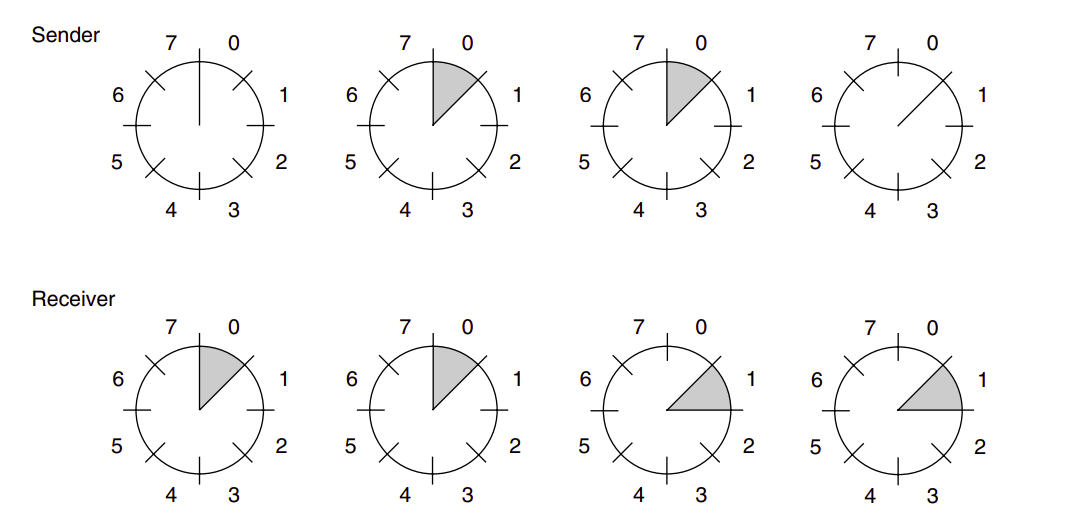
\includegraphics[width=120mm,height=45mm]{Slike/prozori1.png}
            \end{center}
        \end{figure}
        Obašnjenje slike: 
        \begin{itemize}
            \item Prva kolona: Inicijalizacija;
            \item Druga kolona: Šalje se prvi okvir;
            \item Treća kolona: Stigao je ispravan prvi okvir;
            \item Četvrta kolona: Stigao je ispravan ACK okvir.
        \end{itemize}
        Veći prozori omogućavaju protočnu obradu za efikasniju potrebu kanala. Što je veći
        broj prozora to je efikasnija upotreba. Najneefikasniji slučaj je za $W=1$ (posebno
        na dužim kanalima). Optimalno W zavisi od BDP-a. Cilj je da važi $W \geq 2BDP+1$ radi
        što bolje iskorišćenosti.

    \subsection{Protokol ,,1-bitni``}
        Nema odvojenih algoritama pošiljaoca i primoaca, jer je sad dvosmerni kanal i čvorovi
        se ponašaju simetrično. Svodi se na dvosmerni ,,Stani i čekaj``. 
\begin{lstlisting}
void protocol()
{
    seq_nr next_frame_to_send = 0; // dovoljno je da se uzimaju
    seq_nr expected_frame     = 0; // vrednosti 0 ili 1
    frame r, s; 
    packet buffer;
    event_type event;

    from_network_layer(&buffer); // uzima se paket sa mreznog sloja
    s.info = buffer;             // okviruje se paket
    s.seq = next_frame_to_send;  // postavlja se serijski broj
    s.ack = 1-frame_expected;    // zakaci se ACK ser. broj.
    to_physical_layer(&s)        // salje se okvir
    start_timer(s.seq)           // i pokrece se brojac
    while(true)
    {
        wait_for_event(&event);
        if(event == frame_arrival)
        {  
            from_physical_layer(&r);
            if(r.seq == expected_frame) // stigao je validan okvir
            {
                to_network_layer(&r); // prosledjuje se mreznom nivou
                inc(expected_frame);  // ,,pomera se prozor``
            }
            if(r.ack == next_frame_to_send) // poslat okvir je uspesno stigao
            {
                stop_timer(s.seq);           // prekida se brojac
                from_network_layer(&buffer); // uzima se sledeci paket
                inc(next_frame_to_send);     // azurira se ser. br. za slanje
            }
            s.info = buffer;            // uokviruje se sledeci paket koji je
            s.seq = next_frame_to_send; // novi ili stari ako nije stigao ACK
            s.ack = 1-expected_frame;   // zakaci se odg. ACK
            to_physical_layer(&s);      // salje se okvir
            start_timer(&s.seq);        // i pokrece se brojac
        }
    }
}\end{lstlisting}
    \newpage
    Ovaj protokol radi solidno u opštem slučaju. U specijalnom slučaju oba čvora simultano
    započinju komunikaciju. Posledice su duplikati i okinuti brojači (tajmeri). Primer (dobar i loš
    slučaj):
    \begin{figure}[H]
        \begin{center}
            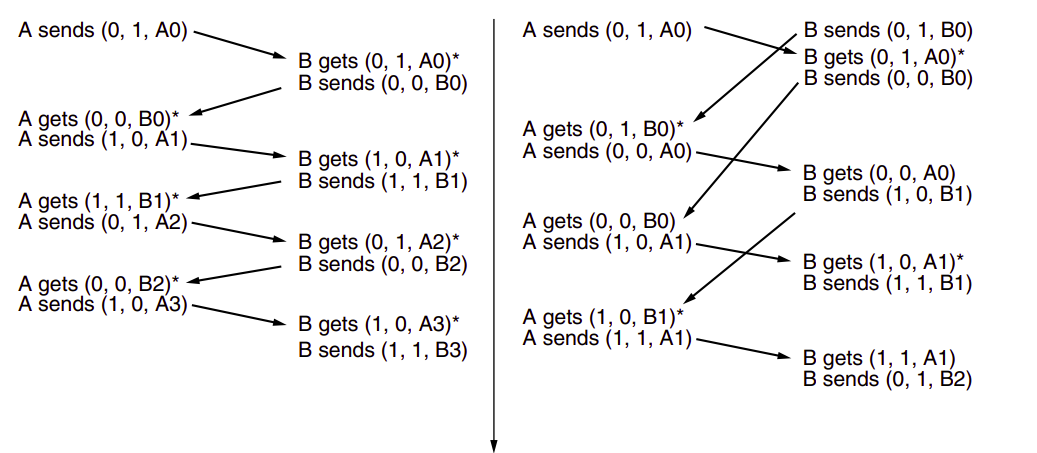
\includegraphics[width=120mm,height=45mm]{Slike/prozori2.png}
        \end{center}
    \end{figure}

    \subsection{Protokol ,,Vrati se N``}
        Pošiljalac šalje niz uzastopnih okvira. Primalac prihvata samo okvire koji stižu redom. 
        Ako neki okvir stigne pre reda onda se on odbacuje. Okviri sa ACK se šalju samo za 
        neodbačene okvire. Kada pošiljaocu istekne tajmer, on opet šalje niz uzastopnih
        okvira. Primalac ima jednostavnu implementaciju sa baferom dimenzije 1. U najgorem slučaju
        moraju opet svi prozori da se šalju, što dovodi do neefikasnosti na kanalu:
        \begin{figure}[H]
            \begin{center}
                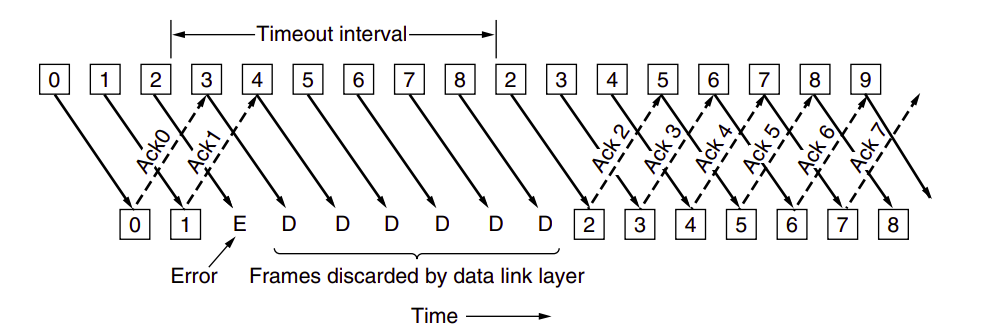
\includegraphics[width=120mm,height=45mm]{Slike/prozori3.png}
            \end{center}
        \end{figure}
    \newpage
    \subsection{Protokol ,,Selektivno ponavljanje``}
        Predstavlja generalizaciju prethodnog protokola. Primalac sada ima bafer dimenzije
        veće od 1 (ako je jednako 1, onda je to ,,Vrati se N`` protokol) 
        i prihvata nekoliko selektivno okvira(sve okvire čiji je redni broj na baferu). 
        Dodatno se koristi \textbf{NAK (negativni ACK)} koji informiše pošiljaoca 
        da ponovo pošalje problematičan okvir. Tada pošiljalac šalje opet okvir koji odgovara
        NAK rednom broju, umesto da čeka da istekne tajmer. Ovo znatno povećava
        efikasnost kanala. Ovaj sistem ima složeniju implementaciju, ali ima veću efikasnost:  
        \begin{figure}[H]
            \begin{center}
                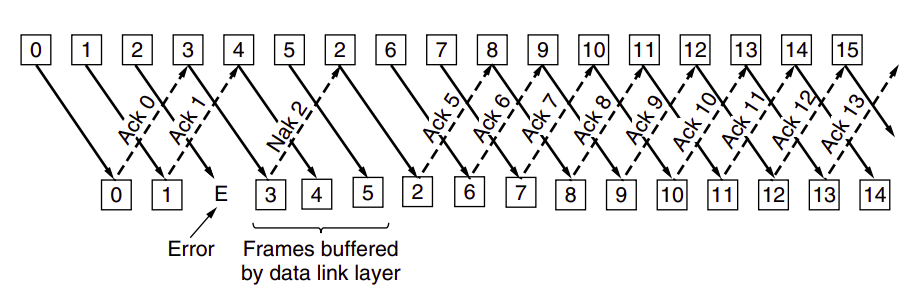
\includegraphics[width=120mm,height=45mm]{Slike/prozori4.png}
            \end{center}
        \end{figure} 
    
\section{MAC podsloj: uloga, alokacija kanala, ALOHA protokol.}
    Mrežni kanali se dele u dve grupe. Prva grupa su \textbf{,,tačka-na-tačku`` (eng. ,,point-to-point``)}
    koji se odnose na komunikaciju između dva čvora. Druga grupa su \textbf{javna emitovanja (eng. broadcast)}
    koja predstavljaju malo komplikovanije sisteme. U ovim sistemima obično čvorovi smetaju jedni
    drugima tj. kvare signal ako šalju signal u isto vreme. \\
    \indent Primer: U grupnim pozivima se često
    dešava da krene više ljudi da govori u isto vreme, nakon što neko završi govor. 
    Ovakvi kanali se nazivaju i \textbf{,,multi access channels`` ili ,,random access channels``}. \\
    \indent Na kanalima sa više čvorova protokoli su zasnovani na tome da određuju ko sledeći
    ,,dobija pravo glasa``. Ovi protokoli pripadaju \textbf{MAC (Medium Access Control) podsloju}.
    Primer: Lan mreže. 
        
    \subsection{protokol ALOHA}
        ALOHA mreža je računarska mreža koja je povezivala havajska ostrva krajem 60-tih godina
        i početkom 70-tih. Povod za izgradnju ove mreže su nedostaci telefonske mreže na havajskim
        ostrvima. Povezivanje ostrva kablovima nije bilo realno rešenje. \\
        
        \textbf{Pravi ALOHA:} Veoma jednostavan sistem: Kada čvor treba da emituje signal? - Kada
        ima nešto što treba da pošalje. Naravno, ovde su kolizije i oštećenja signala neizbežni.
        Čvor koji treba da pošalje okvir emituje signal. Svi čvorovi koji ne šalju signal šlušaju.
        Kada čvorovi prime signal oni ga dalje emituju. Na taj način prvobitni pošiljalac 
        prihvata signal od nekog drugog čvora (isti okvir koje je poslao) i time zna
        da je okvir uspešno poslat. Ako je okvir oštećen onda čvor čeka neko vreme (nasumično
        određeno) i šalje opet signal. \underline{Problem:} Svaki put kada dva čvora žele da pošalju okvir,
        dešava se kolizija, čime su okviri uništeni. Primer sa pet čvorova (A, B, C, D, E):
        \begin{figure}[H]
            \begin{center}
                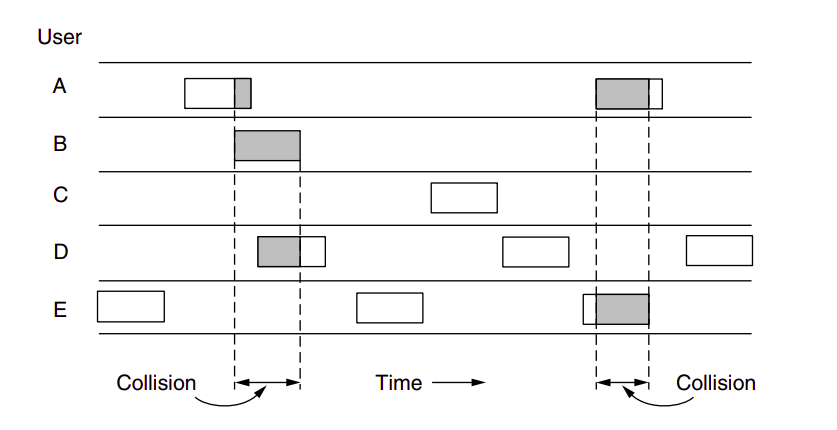
\includegraphics[width=120mm,height=45mm]{Slike/aloha1.png}
            \end{center}
        \end{figure}
        Ovaj sistem radi dobro ako je opterećenje mreže malo. Efikasnost ove mreže je 18\% tj.
        18 od 100 okvira ne bude uništeno. \\

        \textbf{Diskretizovan ALOHA:} Jednostavno unapređenje sistema. Potrebno je da se
        čekanje za ponovno slanje diskretizuje u slotove jednakih dužina. Svaki čvor sada
        bira nasumičan slot kada će opet da pošalje okvir. Pažljivim biranjem dužine slota
        efikasnost mreže može da se poveća na 36\%.

\section{CSMA, CSMA/CD, BEB. }
    Postoji posebna grupa protokola koja osluškuje kanal pre nego što šalje signal. Osluškivanje
    kanala je jednostavno kod žičanih, a komplikovano kod bežičnih kanala. Moguće je da
    se kanal osluškuje, a da se ne čuje da neko drugi šalje signal (posledica kašnjenja).

    \subsection{protokol CSMA}
        \textbf{Protokol CSMA (Carrier Sense Multiple Access)} predstavlja poboljšanje ALOHA protokola
        koji osluškuje kanal pre slanja. Postoje više verzija CSMA protokola:
        \begin{itemize}
            \item \textbf{1-persistent CSMA:} Ako čvor treba da pošalje signal, prvo osluškuje
                  kanal i onda reaguje u odnosu na situaciju:
                  \begin{itemize} 
                    \item Ako je kanal slobodan, šalje se signal. 
                    \item Ako kanal nije slobodan, onda se čeka da bude slobodan. 
                    \item Ako se desi kolizija, onda čvor čeka nasumično određeno vreme.
                  \end{itemize}
                  Protokol se zove ,,1-persistent`` zato što šalje signal kada je kanal slobodan
                  sa verovatnoćom 1. Problemi: 
                  \begin{itemize}
                      \item Kolizija se na ovom protokolu dešava ćešće nego što je to inicijalno
                            intuitivno. Primer: Postoje tri čvora u mreži sa oznakama A, B, C.
                            Neka čvor C trenutno šalje signal ostalim čvorovima u mreži tj. 
                            čvoru A i čvoru B. Takođe, neka u tom trenutku čvorovi A i B imaju
                            podatke koje žele da pošalju i čekaju da C završi slanje.
                            Kada C završi slanje, A i B će u isto vreme da krenu da šalju signal
                            što dovodi do kolizije. Ova situacije je relativno česta u gustim
                            mrežama.
                      \item Kvalitet protokola zavisi dosta od kašnjenja signala. Ako signal kasni,
                            onda može da se desi da čvor ne čuje da neko drugi šalje signal (signal
                            kasni) i krene da šalje signal. Tada opet dolazi do kolizije.
                  \end{itemize}
            \item \textbf{nonpersistent CSMA:} Ako čvor treba da pošalje signal, prvo osluškuje
                  kanal. Ako je kanal zauzet, onda umesto da uporno čeka da što pre zauzme kanal,
                  čeka nasumično određeno vreme pre nego što pokuša opet. Rezultat je manje kolizija,
                  ali duže čekanje.
            \item \textbf{p-persistent CSMA:} Ako čvor treba da pošalje signal, prvo osluškuje 
                  kanal. Ako je kanal slobodan onda se sa verovatnoćom \textbf{p} preuzima kanal,
                  odnosno sa verovatoćom \textbf{1-p} se čeka nasumično određeno vreme pre nego
                  što čvor pokuša opet da preuzme kanal. Ovaj protokol predstavlja hibrid 
                  prethodna dva protokola. 
        \end{itemize}
        \textbf{Upoređivanje protokola:}
        \begin{figure}[H]
            \begin{center}
                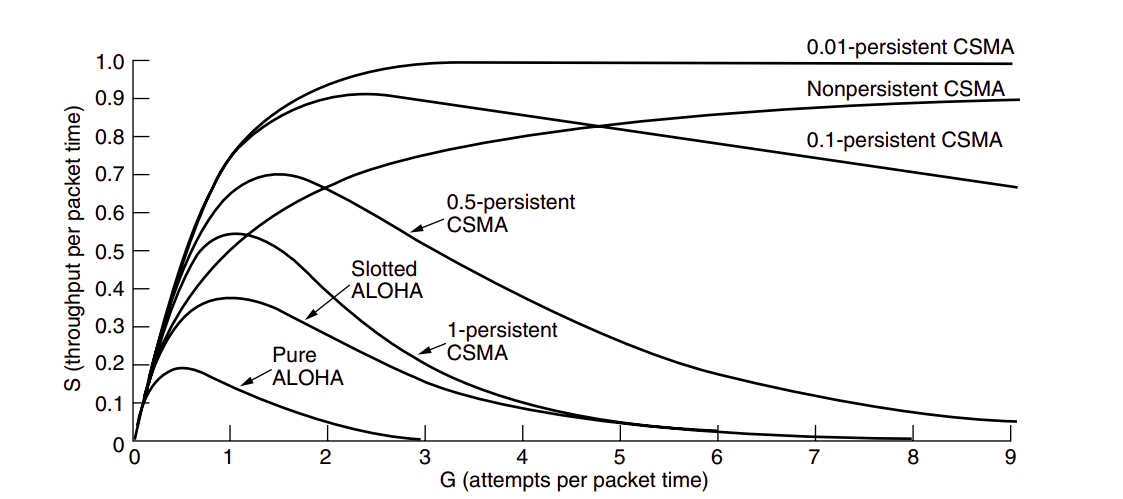
\includegraphics[width=120mm,height=45mm]{Slike/broadcast1.png}
            \end{center}
        \end{figure}
    \subsection{protokol CSMA/CD}
        \textbf{Protokol CSMA/CD (Carrier Sense Multiple Access With Collision Detection)} predstavlja 
        poboljšanje osnove verzije CSMA. Razlika u odnosu na klasičan CSMA je što je 
        prenos prekida čim se primeti da je nastala kolizija. Nakon Primećenje kolizije čvorovi
        koji su prethodno slali podatke čekaju nasumično određeno vreme pre nego što opet
        pokušaju da šalju signal. 
    
    \subsection{Binarno eksponencijalno odlaganje (BEB)}
        \textbf{Binary Exponential Backoff} predstavlja još jedno poboljšanje na osnovni CSMA model (CSMA/CD). 
        Svaki čvor kada se primeti koliziju primenjuje sledeći algoritam:
        \begin{itemize}
            \item Prva kolizija: Čvor čeka 0 ili 1 vremenska okvira (nasumično odabrano).
            \item Druga kolizija: Čvor čeka između 0 i 3 vremenska okvira (nasumično odabrano).
            \item Treća kolizija: Čvor čeka između 0 i 7 vremenska okvira (nasumično odabrano).
            \item ...
            \item N-ta kolizija: Čvor čeka između 0 i $2^{N-1}$ vremenska okvira (nasumično odabrano).
        \end{itemize}
        Opseg intervala brzo raste zbog čega dolazi do dobre procene njegove idealne dužine. Veoma
        efikasan u praksi.

\section{MAC protokoli zasnovani na redosledu: ,,Token Ring``}
    Problem kod CSMA protokola je što je loš pod velikim opterećenjem
    zbog visokih dodatnih troškova (puno kolizija) i variranja vremenskog pristupa. 
    Postoje MAC protokoli koji ne koriste slučajnost već su bazirani na redosledu. Definiše
    se uređenje prema kojem čvorovi šalju ako imaju nešto da pošalju (ili samo propuste prioritet ako
    nemaju šta da pošalju). \\
    \indent Prednosti protokola sa redosledom je što rade efikasnije pod velikim opterećenjem.
    Garantovano je da će svi čvorovi biti usluženi u unapred definisanom vremenu. \\
    \indent Mane protokola sa redosledom je složenost (može da se izgubi token ili slično). Takođe je
    relativno visok dodatni trošak pri malom opterećenju. \\
    \indent U praksi se protokoli sa redosledom obično isprobavaju kao poboljšanje. Međutim, protokoli
    sa slučajnošću se obično teško nadmašuju (jedostavni i dovoljno dobri, skalabilni). 

    \subsection{Protokol ,,Token Ring``}
        Koristi se topologija mreže za definisanje prioriteta po kojem čvorovi mogu da šalju podatke.
        Svi čvorovi su spojeni u jedan prsten. Token kruži u okviru prstena prolažeći kroz čvorove.
        Proces:
        \begin{itemize}
            \item Čvor prima token od svog prethodnika čime dobija prioritet da šalje okvir.
            \item Ako čvor ima okvir koji čeka da bude poslat, onda čvor šalje taj okvir pre nego
                  što prosledi token (samim tim i prioritet) sledećem čvoru. 
            \item Ako čvor nema okvir koji čeka da bude poslat, onda čvor samo prosleđuje token 
                  sledećem čvoru.
        \end{itemize} 
        \begin{figure}[H]
            \begin{center}
                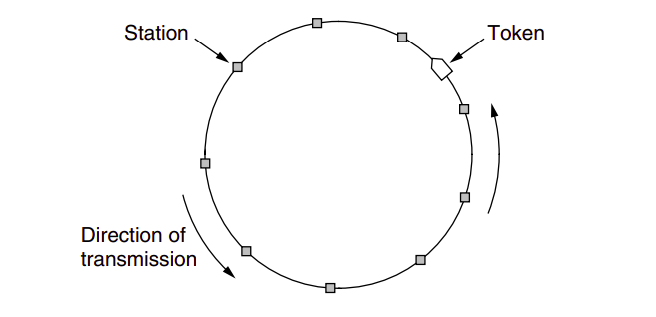
\includegraphics[width=120mm,height=45mm]{Slike/token.png}
            \end{center}
        \end{figure}
        Ovde okviri putuju u istom smeru kao i token. Kako okviri ne bi putovali beskonačno u okviru
        mreže, oni moraju da budu sklonjeni sa mreže. Jedan način je da skine token sa mreže kada čvor (primalac) 
        primi okvir. Drugi način je da sam čvor, pošiljalac skine sa mreže okvir nakon
        što taj okvir obrne krug.\\

        Nije nužno potrebno da kanal bude fizički prsten. Umesto toga je moguće koristiti dugu 
        magistralu gde svaki čvor šalje token sledećem predefinisamo sledbeniku. Ovaj protokol se
        naziva \textbf{,,Token Bus``}.

\newpage
\section{MAC protokoli za bežične mreže}
    Problem kod bežičnih mreža je teško detektovanje kolizije kada se ona dešava (Signal koji
    stiže do čvora može biti veoma slab). Zbog toga nije moguće koristiti CD dodatak uz CSMA.
    Nažalost, takođe nije moguće koristiti CSMA protokol. Primer: Mreža se sastoji od četiri
    čvora A, B, C i D: 
    \begin{figure}[H]
        \begin{center}
            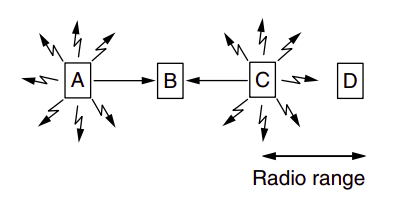
\includegraphics[width=60mm,height=25mm]{Slike/abcd1.png}
        \end{center}
    \end{figure}
    U ovom slučaju čvorovi A i C pokušavaju da šalju signal čvoru B koristeći CSMA protokol. Ako 
    A počne da šalje signal, a C u tom trenutku sluša kanal, onda C neće čuti signal koji dolazi
    od A. Tada C može da pokuša da šalje signal čvoru B. Pošto A i C šalju signal u isto vreme
    dolazi do kolizija signala pri čemu oba okvira (od A i C) bivaju oštećena. Ovaj problem se 
    naziva \textbf{,,problem sakrivenog čvora`` (,,hidden terminal problem``)}. \\
    \indent Drugi Primer: Mreža se sastoji od istih čvorova:
    \begin{figure}[H]
        \begin{center}
            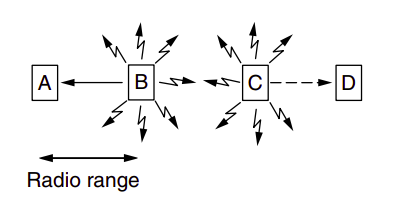
\includegraphics[width=60mm,height=25mm]{Slike/abcd2.png}
        \end{center}
    \end{figure}
    U ovom slučaju čvor B želi da šalje signal čvoru A, a čvor C želi da šalje signal čvoru D. Ako
    B šalje signal, a C u tom trenutku sluša da li neko šalje signal, onda će C čuti signal
    koji stiže od B i pogrešno će zaključiti da se signal ne može slati čvoru D (ne može oštetiti
    signal koji stiže od B ka A, jer je A previše daleko). Ovaj problem se naziva \textbf{,,problem 
    izloženog čvora`` (exposed terminal problem)}.\\
    \indent Kod žica detekcija kolizija (i rano obustavljanje) smanjuje dodatne troškove (overhead).
    Kod bežičnog kanala su veći dodatni troškovi, jer rano obustavljanje nije moguće.  
    \begin{figure}[H]
        \begin{center}
            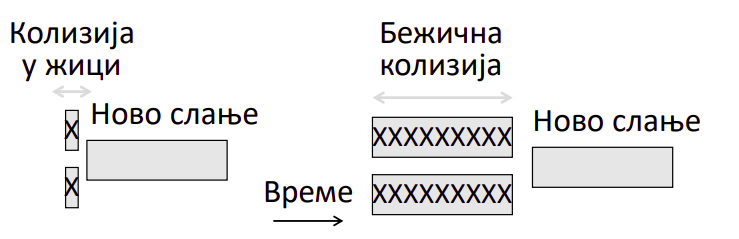
\includegraphics[width=100mm,height=25mm]{Slike/kolizija_zica_bez.png}
        \end{center}
    \end{figure}

    \subsection{Protokol MACA}
        \textbf{Protokol MACA (Multiple Access with Collision Avoidance)} koristi proceduru ,,rukovanja``
        umesto metode CSMA. U praksi se koristi poboljšana verzija MACA (protokol 802.11 tj. WiFi).
        Procedura MACA:
        \begin{enumerate}
            \item Pošiljalac emituje \textbf{RTS okvir (Request To Send)} sa informacijom o dužini okvira
                  koji želi da pošalje.  
            \item Primalac dobija RTS i emituje \textbf{CTS okvir (Clear To Send)} sa informacijom o dužini 
                  okvira koji treba da primi (kopiran do RTS).
            \item Pošiljalac prima CTS i onda počinje slanje.  
        \end{enumerate} 
        \textbf{Kako drugi čvorovi reaguju ca RTS i CTS?}
        \begin{itemize}
            \item Ako neki čvor čuje RTS, onda on mora da sačeka neko vreme da bi
                  onaj čvor koji šalje RTS uspešno prihvatio CTS bez konflikata.
            \item Ako neki čvor čuje CTS, onda on mora da sačeka neko vreme. 
                  Pošto se dužina podatka nalazi u okviru CTS-a, može da 
                  se odrediti koliko dugo treba da se čeka.
        \end{itemize}
        \begin{figure}[H]
            \begin{center}
                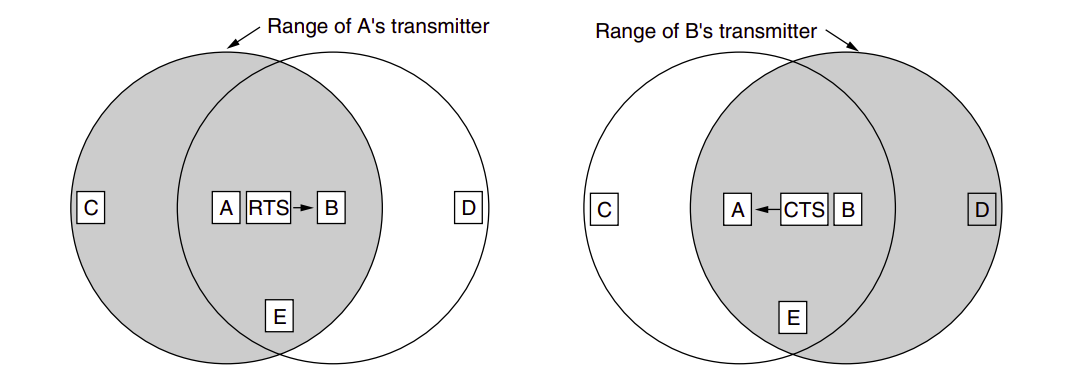
\includegraphics[width=100mm,height=40mm]{Slike/maca1.png}
            \end{center}
        \end{figure}
        Kolizije i dalje mogu da nastanu. Primer: Čvorovi B i C u isto vreme šalju RTS okvire. 
        U tom slučaju dolazi do kolizije i jedan čvor će morati da šačeka nasumično određeno vreme.\\

        \newpage
        \noindent \textbf{MACA i problem sakrivenog čvora:}
        \begin{figure}[H]
            \begin{center}
                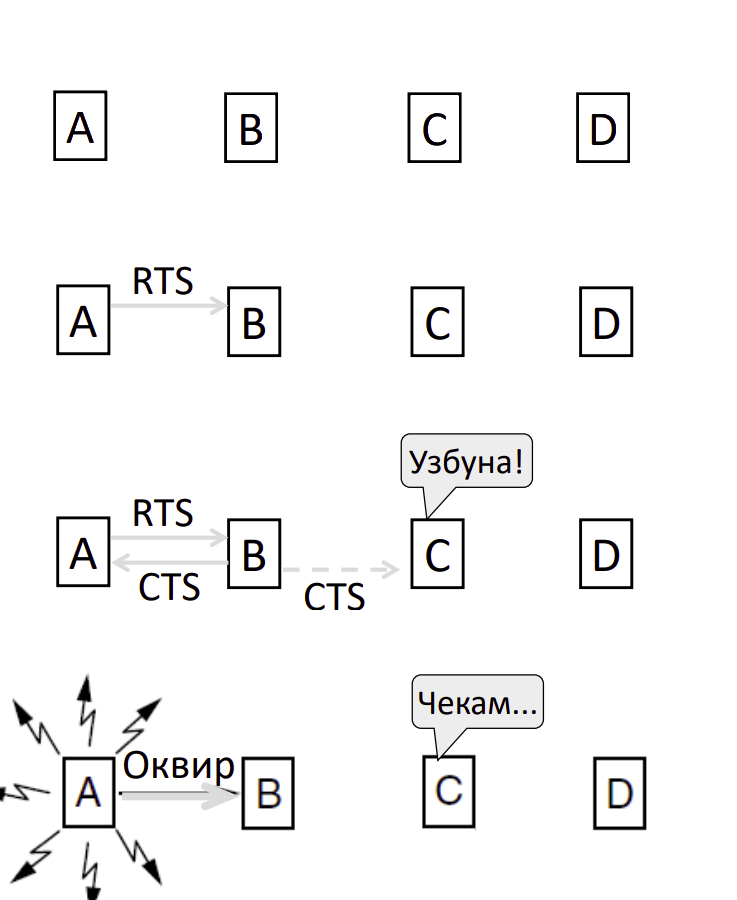
\includegraphics[width=80mm,height=100mm]{Slike/maca_skriveni_cvor.png}
            \end{center}
        \end{figure}

        \newpage
        \noindent \textbf{MACA i problem otkrivenog čvora:}
        \begin{figure}[H]
            \begin{center}
                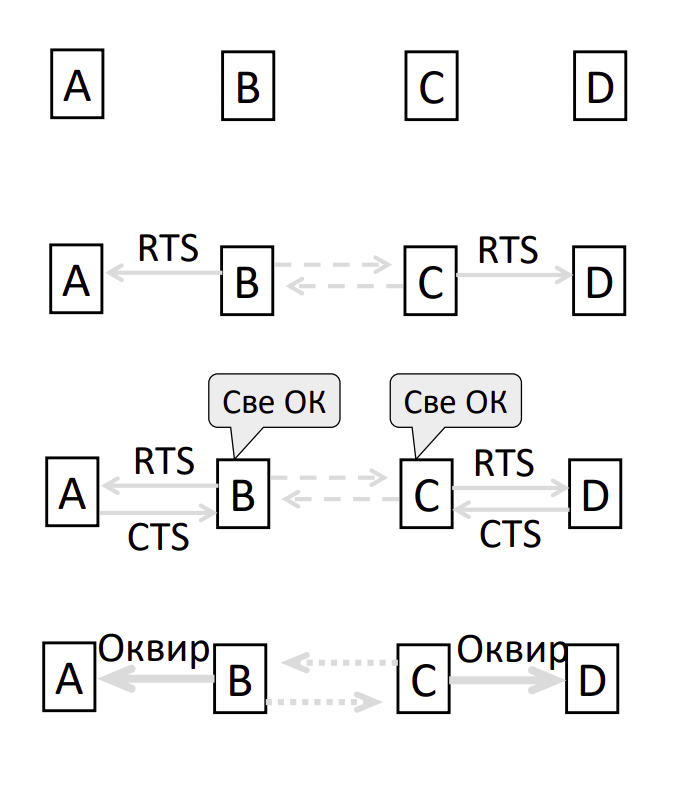
\includegraphics[width=80mm,height=100mm]{Slike/maca_otkriveni_cvor.png}
            \end{center}
        \end{figure}
   
\section{Klasični Eternet - IEEE 802.3}
    Najpopularniji vid organizovanja LAN mreža tokom 80-tih i 90-tih godina. Protok oko 10Mb/s
    preko deljenog koaksijalnog kabla. Koristi \textbf{,,CSMA/CD sa BEB``} model. \\

    Razlika u odnosu na dosadašnje okvire je što se oni sastoje od adrese pošiljaoca i
    adrese primaoca (ovo nije potrebno za ,,point-to-point`` protokole). Za detekciju 
    grešaka se koristi CRC-32. Ne koristi ACK sistem, jer se to ostavlja višim slojevima.
    \begin{figure}[H]
        \begin{center}
            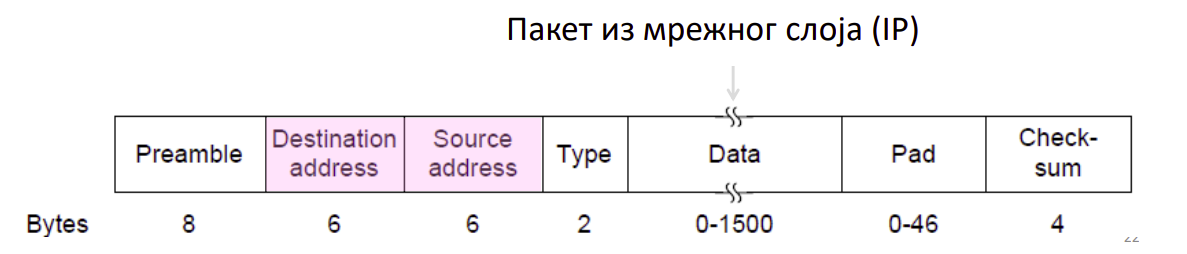
\includegraphics[width=120mm,height=25mm]{Slike/eternet1.png}
        \end{center}
    \end{figure}
    
\section{Moderni (komutirani) Eternet}
    Moderni Eternet ne koristi MAC, već skretnice (switches). Kanali se na hardverskom 
    nivou razdvajaju. 

    \subsection{Razvodnik (HUB)}
        Najlakši način da se povežu čvorovi u mreži je da se koristi jedan dovoljno dugačak kanal
        preko kojeg čvorovi mogu da šalju okvire. Ovo rešenje donosi mnogo problema prilikom
        prekida na kanalu (nije lako locirati). \\
        \indent Bolje rešenje se dobija koristeći razvodnik (hub). Razvodnik je kutija sa 
        više ulaza/izlaza preko koje mogu da se povezuju čvorovi. Funkcija i implementacija 
        razvodnika je jednostavna. Kada stigne neki okvir do njega on ga prosleđuje svim ostalim
        čvorovima koji su prikačeni na njega.
        \begin{figure}[H]
            \begin{center}
                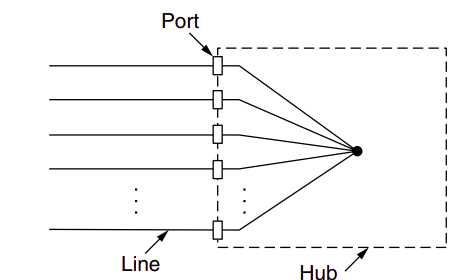
\includegraphics[width=80mm,height=40mm]{Slike/hab.png}
            \end{center}
        \end{figure}
        \noindent \textbf{Prednosti:}
        \begin{itemize}
            \item Značajno ušteđuje na količini materijala potrebno da se spoje čvorovi (potrebna 
                  manja ukupna dužina kanala mreže). 
            \item Dodavanje i uklanjavanje čvorova je poprilično jednostavno.
            \item Pronalaženje prekida je lakše. Ako se izgubi kontakt sa jednim čvorom, onda
                  je prekid na žici između čvora i razvodnika ili je čvor otkazao. Ako se
                  izgubi kontakt na nivou cele mreže, onda je razvodnik otkazao.
        \end{itemize}
        Nažalost, razvodnik ne povećava kapacitet i skalabilnost mreže, jer predstavlja
        logički ekvivalent dugog kabla. Razvodnik i dalje zahteva protokol CSMA/CD, jer kolizije
        pri slanju ostaju. 

    \subsection{Skretnica (Switch) - opšte}
        Skretnica izgleda isto kao razvodnik i čvorovi se povezuju na isti način. Prednost skretnice
        je u njenoj unutrašnjoj implementaciji. Umesto da se okvir šalje svim čvorovima u mreži, 
        skretnica pamti adrese svojih čvorova i prosleđuje okvir samo primaocu. Skretnica ima 
        odgovaraujući algoritam za pamćenje adresa. Svi čvorovi sa skretnicom su obično povezani
        preko punog dupleksa. To znači da svaki čvor može da šalje okvire bez brige da li
        će doći do kolizije. Posledica ovo je da CSMA/CD gubi svoj smisao u nedostatku kolizija.
        \begin{figure}[H]
            \begin{center}
                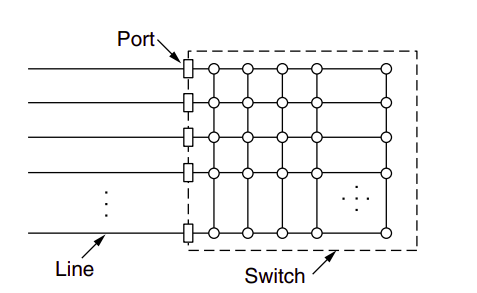
\includegraphics[width=80mm,height=40mm]{Slike/skretnica.png}
            \end{center}
        \end{figure}
        Prednosti u odnosu na razvodnik po performansama (sve prednosti razvodnika u odnosu na
        jedan dugi kanal važe i za skretnicu):
        \begin{itemize}
            \item Nema kolizije i time je kapacitet bolje iskorišćen.
            \item Može da šalje više okvira u isto vreme.
        \end{itemize}
        Skretnica ima bafere za ulaz i izlaz u slučaju da ima više okvira od jednog čvora koji 
        stižu ili u slučaju da više okvira treba da se pošalju jednom čvoru (u slučaju prelivanja
        bafera gube se okviri).
        \begin{figure}[H]
            \begin{center}
                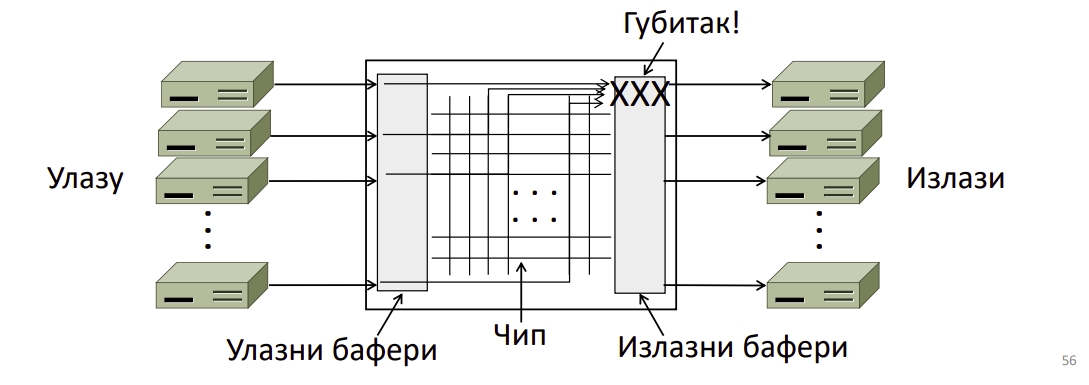
\includegraphics[width=80mm,height=40mm]{Slike/skretnica_baferi.png}
            \end{center}
        \end{figure}

    \subsection{Skretnica (Switch) - učenje unazad}
        Za prosleđivanje okvira se koristi tabela relacija između
        broja porta i adrese okvira. Da bi se popunila tabela, posmatraju se adrese i portovi
        čvorova koji šalju okvire. Ako se za zadatu adresu u tabeli nalazi priduženi port, onda
        se okvir šalje samo njemu, a u suprotnom se šalje svim čvorovima.\\
        \indent Data je mreža sa četiri čvora. Demonstracija učenja tabele relacije. Neka
        čvor A šalje okvir čvoru D:
        \begin{figure}[H]
            \begin{center}
                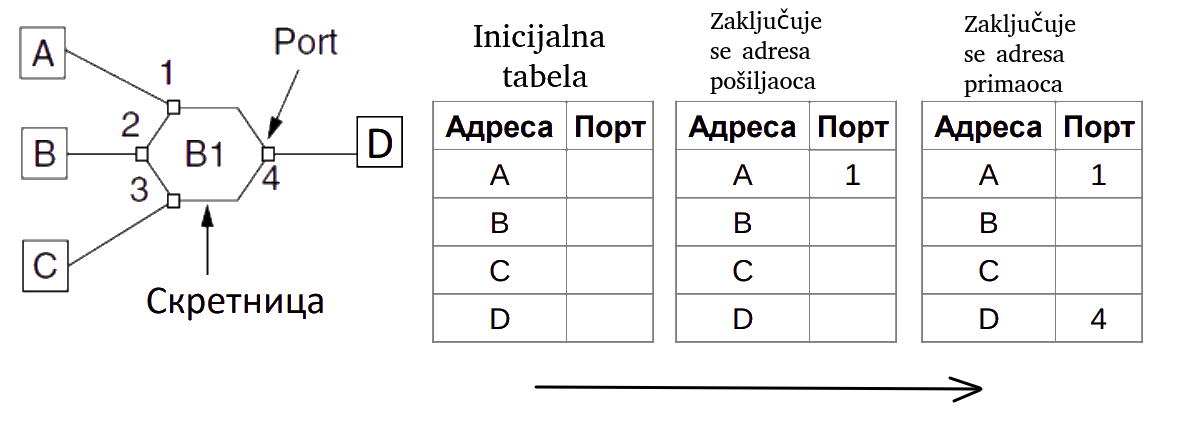
\includegraphics[width=120mm,height=40mm]{Slike/skretnica_ucenje.png}
            \end{center}
        \end{figure}

        \noindent \textbf{Detaljno objašnjenje procesa sa slike:} 
        \begin{itemize}
            \item Inicijalno skretnica ima praznu tabelu.
            \item Čvor A šalje okvir čvoru D (okvir sadrži adresu primaoca i pošiljaoca).
            \item Okvir stiže iz čvora A. Adresi čvora A se dodeljuje port koji služi
                  za kasnije preslikavanje.
            \item \underline{Problem: Skretnica ne zna koji port vodi ka čvoru D!}
                  U ovakvim situacijama se skretnica ponaša kao razvodnik i šalje okvir svim ostalim
                  čvorovima. 
            \item Čvorovi koji dobiju okvir od skretnice, a ne odgovara im adresa pošiljaoca,
                  jednostavno odbacuju okvir. Čvoru D odgovara adresa pošiljaoca i on šalje
                  odgovor čvoru A. 
            \item Skretnici stiže okvir od čvora D. Adresi čvora D se dodeljuje port koji služi
                  za kasnije preslikavanje. 
            \item Skretnica prosleđuje okvir čvoru A.
        \end{itemize}

        \begin{figure}[H]
            \begin{center}
                \includegraphics[width=120mm,height=40mm]{Slike/skretnice_komplikovanija_mreza.png}
            \end{center}
        \end{figure}
        Na jednoj mreži mogu da se nalaze više skretnica i razvodnika. Svaka skretnica ima svoju
        nezavisnu tabelu.

    \subsection{Eliminacija petlji}
        U slučaju komplikovanih mreža može doći do petlji. Rešenje ovog problema je formiranje
        razapinjujećeg stabla. Razapinjujeće stablo nema petlje, ali povezanost u okviru mreže ostaje 
        (ako je postojao neki put između dva čvora, onda i dalje postoji neki put između
        ta dva čvora, ali ne nužno isti put). 
        \begin{figure}[H]
            \begin{center}
                \includegraphics[width=120mm,height=40mm]{Slike/skretnice_petlje.png}
            \end{center}
        \end{figure}  
        
\section{Mrežni sloj: uloga, motivacija, rutiranje i prosleđivanje (ukratko), tipovi servisa na
mrežnom sloju, objašnjenja i njihov uporedni odnos.}
    Jedinica podataka koja se koristi na nivou mrežnog sloja je paket. Uloga mrežnog sloja
    je da šalje paket od izvora do odredišta. Mrežni sloj je najniži sloj koji prosleđuje tako
    podatke (sloj veze prosleđuje okvire sa jednog kraja žice na drugi). Da bi se ova uloga uspešno
    obavljala, mrežni sloj zalazi u topologiju mreže kako bi izabrao dobre puteve, balansirao
    zagušenja na nivou mreže i omogućio komunikaciju mreža sa različitim tehnologijama.\\
    
    \textbf{Problemi sa skretnicama:} Teoretski, koristeći veze i skretnice je dovoljno da se izgradi
    mreža koja može da razmenjuje podatke. Problemi:
    \begin{itemize}
        \item Loša skalabilnost: Tabela relacije kod skretnica bi postala ogromna. Takođe skretnice
              bi u početku se ponašale kao razvodnici dok ne nauče tabele relacije.
        \item Ne mogu da se kombinuju različiti tipovi mreža (različite tehnologije). Primer, Eternet
              i 3G.
        \item Ne postoji kontrola saobraćaja koja bi smanjila zagušenje u okviru mreže.
    \end{itemize}

    \textbf{Rutiranje i prosleđivanje (ukratko):} Rutiranje je proces u kojem se odlučuje u 
    kom pravcu treba poslati podatke. Prosleđivanje je proces slanja paketa na osnovu 
    lokalne tabele. \\
    
    \subsection{Tipovi servisa na mrežnom sloju}
        Uslovi koje servisi koje mrežni sloj pruža transportnom sloju treba da ispunjavaju:
        \begin{enumerate}
            \item Servisi treba da budu nezavisni od tehnologije rutera.
            \item Transportni sloj ne mora da zna broj, tip ili topologiju rutera.
            \item Adrese koje koristi transportni sloj bi trebalo da koriste
                  neki ujednačeni plan za brojanje.
        \end{enumerate}
        \textbf{Postoje dva tipa servisa koje mrežni sloj nudi transportnom sloju:}
        \begin{itemize}
            \item \textbf{Datagrami (Connectionless Service):} Servis bez uspostavljenja 
                  veze (kao pošta). Svaki paket se šalje nezavisno. Paket sadrži ciljnu adresu
                  na osnovu koje usmerivač (ruter) prosleđuje paket dalje koristeći dinamičnu
                  (menja se vremenom) \textbf{tabelu prosleđivanja (forwarding table)}. Ukoliko
                  jedan čvor šalje više paketa nekom drugom čvoru, onda ne mora svaki paket
                  da putuje istim putem. \underline{Primer:} Treba da se pošalje neki veliki podatak koji
                  se dobija od transportnog sloja. Taj podatak može da stane u par paketa, pa
                  se tako i šalje. Svaki od ovih paketa može da ima različitu putanju.
            \item \textbf{Virtuelna kola (Connection-Oriented Service):} Servis sa uspotavljenom
                  vezom (kao fiksna telefonija). Paketi, koji se šalju koristeći ovaj servis,
                  putuju istom putanjom koja je određena kada je uspostavljena virtuelna konekcija.
                  Prilikom uspostavljenja virtuelne veze svi usmerivači (ruteri) u okviru
                  putanje trebaju da imaju informaciju o toj putanji. Paketi sadrže kratak identifikator
                  virtuelnog kola (globalno značenje). U slučaju da dva različita čvora žele
                  da uspostave konekciju sa jednim istim čvorom, potrebno je da svako kolo
                  ima svoj identifikator kako bi se razlikovalo od ostalih kola.  
        \end{itemize}
        Oba servisa koriste \textbf{,,sačuvaj-i-prosledi`` (,,store-and-forward``)} tehniku, gde
        usmerivači (ruteri) dobijaju paket i privremeno ga čuvaju (ruteri imaju svoje bafere)
        sve dok ga ne proslede dalje.

    \subsection{Internet protokol (IP)}
    Mrežni sloj koristi datagramski servis. Paket ipv4 ima 32-bitnu adresu i 
    obično je velik oko 1.5KB.
    \begin{figure}[H]
        \begin{center}
            \includegraphics[width=100mm,height=60mm]{Slike/ip_protokol.png}
        \end{center}
    \end{figure}
    \textbf{Elementi:}
    \begin{itemize}
        \item \textbf{Version:} verzija ipv4 (češća) ili ipv6.
        \item \textbf{IHL:} dužina zaglavlja.
        \item \textbf{Differentiated Services:} informacije o klasi servisa i zagušenju.
        \item \textbf{Total Length:} Ukupna dužina paketa (sa zaglavljem).
        \item \textbf{Identification field:} informacija o tome kome paket pripada
              kada stigne na odredište.
        \item \textbf{DF, MF, Fragment offset:} dodatne informacije o fragmentu.
        \item \textbf{Time to Live:} definiše se životni vek paketa (u slučaju da se izgubi,
              da ne bi lutao).
        \item \textbf{Protocol:} UDP ili TCP (ili neki treći).
        \item \textbf{Header Checksum:} za detekciju greške.
        \item \textbf{Source Adress:} Ip adresa pošiljaoca.
        \item \textbf{Destination Adress:} Ip adresa primaoca.
        \item \textbf{Options:} Dodatne informacije koje zavise od verzije IP protokola.
        \item \textbf{TCP segment}.
    \end{itemize}

    \subsection{Datagrami i virtuelna kola}
        Virtuelno kolo zahteva pripremu da se uspostavi veza. Ova priprema zahteva dodatne resurse.
        Međutim, kada se cena plati, za usmeravanja u okviru kola je dovoljno da se koristi
        oznaka za usmeravanja, umesto cele adrese koja se koristi u slučaju datagrama. Virtuelna
        kola su više osetljiva na otkazivanje rutera u okviru definisane putanje. U tom slučaju
        veza propada (datagrami nemaju ovaj problem). Takođe, datagrami omogućavaju veću
        fleksibilnost kod razrešavanja zagušenja u okvir mreže. Zaključak: oba servisa
        imaju svoje prednosti i mane.   
        \begin{figure}[H]
            \begin{center}
                \includegraphics[width=120mm,height=60mm]{Slike/divk.png}
            \end{center}
        \end{figure}

    \newpage
    \subsection{Povezivanje različitih mreža (međumreža)}
        \noindent Mreže mogu da se razlikuju u mnogo aspekata:
        \begin{itemize}
            \item Tip servisa (datagrami, virtuelna kola);
            \item Adresiranje;
            \item Kvalitet usluge (QOS: Quality of Service);
            \item Veličina paketa;
            \item Sigurnost (enkripcija).
        \end{itemize}
        Potrebno je da postoji preslikavanje između IP adresa i oznaka virtuelnog kola. 
        Internet servis provajderi (ISP) često koriste virtuelna kola kako bi grupisali IP
        saobraćaj i brže preneli podatake:
        \begin{figure}[H]
            \begin{center}
                \includegraphics[width=120mm,height=40mm]{Slike/grupisanje_paketa.png}
            \end{center}
        \end{figure}

\section{IP adrese i prefiksi}
    Koriste se dve verzije IP adresa: IPv4 (32-bitna adresa) i IPv6 (128-bitna adresa). Adresa
    IPv4 se trenutno više koristi, a u procesu je prelazak na IPv6 verziju. Notacija za IPv4 adresu
    je u obliku kvarteta dekadnih brojeva, gde je svaki dekadni broj iz opsega [0, 255].  
    \begin{figure}[H]
        \begin{center}
            \includegraphics[width=120mm,height=30mm]{Slike/ipv4_notacija.png}
        \end{center}
    \end{figure}

    \subsection{Prefiksi}
        Adrese se grupišu u blokove pod nazivom \textbf{prefiksi}. L-bitni prefiks je grupa adresa
        koje imaju isti prefiks dužine L bita. To znači da L-bitni prefiks ima $2^{32-L}$ 
        različitih adresa. Notacija grupa je u obliku: ,,IP adresa/dužina prefiksa``. Primer:
        128.13.0.0/16 ima fiksiran prefiks prvih 16 bitova (prva 2 dekadna broja) tako da je
        opseg od 128.13.0.0 do 128.13.255.255. Primer: 128.13.0.0/32 je jedinstvena adresa. \\
        \indent Jedna IP adresa pripada različitim prefiksima. Što je prefiks duži, to je 
        opseg adrese manji (specifičniji prefiks). Najspecifičniji prefiks je dužine 32 tj.
        konkretna adresa. Što je prefiks kraći, to je opseg adrese veći (manje specifičan prefiks).
        Najmanje specifičan prefike je dužine 0 tj. cela mreža (Internet).\\

        \noindent \textbf{Stari sistem za grupisanje u klase fiksne dužine:}
        \begin{itemize}
            \item Klasa A, $2^{24}$ adresa.
            \item Klasa B, $2^{16}$ adresa.
            \item Klasa C, $2^{8}$ adresa (odgovara LAN mreži).
        \end{itemize}
        \begin{figure}[H]
            \begin{center}
                \includegraphics[width=120mm,height=30mm]{Slike/ip_prefiksi_stara_klasifikacija.png}
            \end{center}
        \end{figure}

    \subsection{Privatne i javne IP adrese}
        \begin{itemize}
            \item \textbf{Javna IP adresa:} Jedinstvena na nivou celog interneta. Mora se dodeliti
                  pre upotrebe (regulatorno telo). Ove mreže su većim delom potrošene, ali 
                  polako se prelazi na IPv6 čime će neštašica biti rešena.
            \item \textbf{Privatna IP adresa:} Nisu jedinstvene na nivou celog interneta, ali
                  jesu jedinstvene na nivou manjih mreža (mreža firme, kućna mreža, \dots).
                  Potrebna je bar jedna javna IP adresa i \textbf{NAT (Network Address Translation)} da bi
                  se neko iz ovakve mreže povezao na Internet.
        \end{itemize}

        Svetsko regulatorno telo \textbf{IANA (Internet Assigned Numbers Authority)}, odeljenje u okviru
        \textbf{ICANN (Internet Corporation for Assigned Names and Numbers)} neprofitabilne korporacije,
        dodeljuje ceo opseg adresa regionalnim telima. Regionalna tela dodeljuju opsege 
        kompanijama u regionu. Kompanije dodeljuju konkretnim računarima. 
        \begin{figure}[H]
            \begin{center}
                \includegraphics[width=120mm,height=30mm]{Slike/iana.png}
            \end{center}
        \end{figure}

\section{IP prosleđivanje}
    Internet je mreža koja ima barem milion čvorova. Jedan ruter ne može da ima tabelu svih čvorova
    tolike mreže (ovo je moguće za manje mreže). Odakle proizilazi problem tabela rutiranja. 
    Jedno rešenje bi bilo da se napravi hijearhija za IP adrese: država, opština/region, grad, 
    mreže u okviru grada i krajnji čvor. Svaki ruter treba da zna:
    \begin{itemize}
        \item Kako doći iz svoje u drugu državu;
        \item U okviru svoje države, kako doći u drugu opštinu/region;
        \item U okviru svoje opštine ili regiona, kako doći u drugi grad;
        \item U okviru svog grada, kako doći u druge podmreže grada;
        \item U okvir svoje podmreže grada, kako doći do drugih kranjih čvorova. 
    \end{itemize} 
    Ovakva hijearhija bi zahtevala više od 32-bita za realizaciju, ali postoji slična uopštenija
    ideja. Umesto da se manje mreže spajaju u veće mreže, manji prefiske se spajaju u veće 
    (manje specifične) prefikse IP adresa. Ovaj proces se naziva \textbf{agregacija ruta (,,route 
    aggretation``)}. Svaki ruter ima tabelu prefiksa koji mogu da variraju po veličini. Ovaj
    sistem se naziva \textbf{CIDR (Classless Internet Domain Routing)}. Ruteri imaju specifičnije
    prefikse za mreže koje su bliže:
    \begin{figure}[H]
        \begin{center}
            \includegraphics[width=120mm,height=50mm]{Slike/cidr1.png}
        \end{center}
    \end{figure}
    Tabele rutiranja mogu da imaju prefikse koji se poklapaju. Ruter odlučuje u kom
    pravci šalje paket na osnovu \textbf{pravila najdužeg odgovarajućeg prefiksa}. Za svaki paket
    se pronalazi najduži (Najspecifičniji) prefiks koji njemu odgovara i u tom pravcz
    se prosleđuje.
    \begin{figure}[H]
        \begin{center}
            \includegraphics[width=120mm,height=50mm]{Slike/cidr2.png}
        \end{center}
    \end{figure}
    \textbf{Kompromis vremenske i prostorne složenosti:} Kompaktnije tabele imaju podrazumevanije
    ponašanje (manje specifični prefiksi), zauzimaju manje prostora i manje su vremenski efikasne.
    Velike tabele su specifičnije (više specifični prefiksi) ponašanje, zauzimaju više prostora
    i vremenski su efikasnije.

\section{ARP i DHCP}
    \noindent \textbf{Dva problema koji se pojavljuju na mrežnom sloju su:}
    \begin{itemize}
        \item Dodeljivanje IP adrese računaru u mreži (DHCP);
        \item i određivanje adrese u sloju veze (MAC) za ciljnu IP adresu (ARP).
    \end{itemize}

    Svaki računar u mreži ima jedinstvenu \textbf{MAC (Media Access Control) adresu} koja se nalazi
    na \textbf{NIC (Network Interface Controller)} kartici. To znači da se MAC dodeljuje hardverski svakom
    računaru koji treba da koristi internet usluge.

    \subsection{Dodeljivanje IP adrese (DHCP)}
        Svaki čvor u mreži mora da ima neku svoju IP adresu kako bi komunicirao na sloju mreže.
        Moguće je svakom čvoru dodeliti IP adresu statički ili dinamički. Dinamičko dodeljivanje adresa
        je uglavnom boje rešenje.\\
        \indent \textbf{Protokol DHCP (Dynamic Host Configuration Protocol)} dinamički dodeljuje adresu čvoru 
        u okviru mreže. Kada se računar pokrene, on nema svoju IP adresu.
        Da bi dobio adresu on mora da pošalje paket DHCP serveru. Ako taj server nije direktno
        povezan na mrežu, onda računar emituje javnu (broadcast) poruku. Ruteri preusmeravaju
        DHCP zahtev DHCP serveru. Server prihvata paket sa zahtevom i dodeljuje mu slobodnu
        IP adresu. \\
        \indent Nakon nekog vremena računar napušta mrežu i IP adresa se gubi. Posledica ovoga
        je brzo dolaženje do nestašice IP adresa. Zbog toga DHCP protokol dodeljuje IP
        adresu na određeni vremenski period. Ova metoda se naziva \textbf{,,iznajmljivanje`` 
        (,,leasing``)}. Pri isteku roka računar može da zaheva produženje roka. Ako se ne pošalje 
        (uspešno) zahtev za produženje roka, onda se gubi IP adresa. \\

        \noindent \textbf{Detaljniji proces DHCP protokola (three way handshake):}
        \begin{enumerate}
            \item Čvor emituje paket celoj mreži (specijalna adresa za emitovanje je 255.255.255.255).
            \item DHCP server odgovara čvoru ciljano sa predloženom IP adresom. Ova adresa se bira
                  na osnovu njegove MAC adrese i slobodnih IP adresa.
            \item Čvor emituje odgovor da mu odgovara predložena IP adresa (može biti više
                  DHCP servera).
            \item DHCP server potvrđuje i briše adresu iz spiska slobodnih IP adresa.
        \end{enumerate}
        \begin{figure}[H]
            \begin{center}
                \includegraphics[width=80mm,height=60mm]{Slike/dhcp.png}
            \end{center}
        \end{figure}
        Protokol takođe omogućava paralelni rad više repliciranih DHCP servera zarad pouzdanosti
        i efikasnosti. Emituje se REQUEST tako da su sihronizovani.
    
    \subsection{Određivanje adrese u sloju veze za ciljnu IP adresu (ARP)}
        Sloj veze podataka ne ume da radi sa IP adresama. Potrebno je preslikati IP adrese 
        na adresu u sloju veze. Proces:
        \begin{enumerate}
            \item Čvor koji hoće da sazna adresu emituje ciljnu IP adresu.
            \item Onaj ko ima tu IP adresu mu vraća odgovor sa svojom adresom na sloju veze.
        \end{enumerate}
        \begin{figure}[H]
            \begin{center}
                \includegraphics[width=80mm,height=60mm]{Slike/arp.png}
            \end{center}
        \end{figure}
        Moguće su razne optimizacije ARP protokola. Jedna od optimizacije je da se 
        vrši keširanje rezultata u slučaju da se opet traži ista adresa.
        
\section{ICMP i NAT}
    \subsection{Protokol ICMP}
        Operacije nad mrežom su praćene od strane rutera. Ako ruter primeti neku grešku prilikom
        prosleđivanja paketa, onda se taj slučaj prijavljuje pošiljaocu putem \textbf{ICMP (Internet 
        Control Message Protocol) protokola}. Protokol ICMP se takođe koristi za testiranje Interneta
        (primer: \textit{ping}). 
        Mogu se definisati razni tipovi poruka. Svaka ICMP poruka se šalje preko paketa. Problematičan
        paket se odbacuje. \\
        \indent Paket ICMP sadrži tip greške, kod i kontrolni zbir. Postoji indikator kojim
        se ICMP paket razlikuje od ostalih.  
        \begin{figure}[H]
            \begin{center}
                \includegraphics[width=100mm,height=60mm]{Slike/icmp_tipovi.png}
            \end{center}
        \end{figure}

    \newpage
    \subsection{NAT tehnika}
        Povezivanje računara iz lokalne mreže na spoljnu mrežu (primer: Internet) se vrši preko
        \textbf{NAT (Network Address Translation)} tehnike. NAT se izvršava u ruterima.
        Protokol IPv4 omogućava par milijardni 
        ($2^{32}$) dostupnih adresa, što nije dovoljno. Nestašicom IPv4 adresa je motivisan NAT.\\
        \indent NAT održava tabelu preslikavanja unutrašnjih u spoljašnje (i obrnuto) adrese.
        To preslikavanje je zapravo IP+TCP port informacija. Portovi su ovom slučaju neophodni
        da bi preslikavanja bilo ,,1-1``.
        \begin{figure}[H]
            \begin{center}
                \includegraphics[width=80mm,height=40mm]{Slike/nat1.png}
            \end{center}
        \end{figure}
        \noindent \textbf{Kako NAT funkcioniše:}
        \begin{itemize}
            \item \textbf{Unutrašnji IP u spoljašnji IP:} Prilikom slanja podataka iz lokalne mreže,
                  svakom IP paketu se menja adresa pošiljaoca u skladu sa zadatim preslikavanjem.
                  (,,šta računar misli`` $\rightarrow$ ,,šta ISP misli``) 
            \item \textbf{Spoljašnji IP u unutrašnji IP:} Prilikom prihvatanja podataka iz spoljne mreže,
                  svakom IP paketu se se menja adresa primaoca u skladu sa zadatim preslikavanjem.
                  (,,šta ISP misli`` $\rightarrow$ ,,šta računar misli``) 
        \end{itemize}
        \begin{figure}[H]
            \begin{center}
                \includegraphics[width=120mm,height=50mm]{Slike/nat2.png}
            \end{center}
        \end{figure}
        \textbf{Prednosti NAT-a:}
        \begin{itemize}
            \item Smanjuje potrebe za javnim IP adresama (dovoljna je jedna po domaćinstvu).
            \item Lako se instalira.
            \item Često ima u sebi neki vid zaštite od upada (firewall).
            \item Pomaže po pitanju privatnosti.
        \end{itemize}
        \textbf{Mane NAT-a}:
        \begin{itemize}
            \item Narušena je ,,čistoća`` slojevitosti! Radi na mrežnom sloju, a barata sa TCP portovima.
            \item Paketi mogu da se primaju samo ako je prethodno bilo poslatih paketa tj. mapiranje se
                  vrši preko odlazećih paketa.
            \item Teško koristiti servere preko NAT-a (rešenje: port-forwarding, VPN, SSH tunneling).
        \end{itemize}

\section{Rutiranje: mehanizmi alokacije protoka, modeli isporuke, ciljevi rutiranja, principi
        dizajna algoritama rutiranja, rutiranje sa najkraćim putevima (najmanjim troškom),
        Dijkstrin algoritam. }
    Jedna od glavnih funkcija mrežnog sloja je rutiranje. \textbf{Rutiranje} je proces (algoritam)
    kojim se određuje putanja paketa tj. u kom pravcu treba poslati paket. Ključni aspekt 
    rutiranja je alokacija protoka. Prilikom alokacije protoka treba imati na umu 
    otkazivanje čvorova. 
    \begin{figure}[H]
        \begin{center}
            \includegraphics[width=120mm,height=50mm]{Slike/rutiranje1.png}
        \end{center}
    \end{figure}
    \textbf{Statično rutiranje (neprilagođavajući algoritmi):} Putevi od čvora A do čvora B su unapred
    definisani (umesto da se određuju na osnovu promena topologije i zagušenja mreže). Ovaj način 
    rutiranja je jako osetljiv na otkaze čvorova. Koriste se samo kada je očigledno kako treba 
    rutirati.\\
    \indent \textbf{Dinamičko rutiranje (prilagođavajući algoritmi):} Suprotno od statičkog
    rutiranja, prilagođavajući algoritmi uzimaju u obzir promene topologije i zagušenja mreže 
    (neki jednostaviji modeli uzimaju u obzir samo promene topologije). 

    \subsection{Modeli isporuke}
    Koriste se razlačiti algoritmi rutiranja za različite modele:
    \begin{figure}[H]
        \begin{center}
            \includegraphics[width=120mm,height=40mm]{Slike/rutiranje2.png}
        \end{center}
    \end{figure}

    \subsection{Ciljevi rutiranja}
    \begin{itemize}
        \item \textbf{Tačnost:} Pronalazi se putanja koja radi.
        \item \textbf{Efikasnost:} Racionalno se troši protok.
        \item \textbf{Ravnopravnost:} Podjednaka prava čvorova tj. izbegava se izgladnjivanje čvorova.
        \item \textbf{Brza konvergencija:} Brz oporavak nakon promena (novi čvor, otkazan čvor).
        \item \textbf{Skalabilnost:} Radi dobro i kada mreža raste.
    \end{itemize}

    \subsection{Principi dizajna algoritama rutiranja}
    \noindent \textbf{Decentralizovani i distribuirani:}
    \begin{enumerate}
        \item Čvorovi su ruteri. Korisnički računari se ne razmatraju (podaci od poslednjeg
              rutera do računara se razmatra u okviru sloja veze).
        \item Svi čvorovi su ravnopravni tj. nema bitnijih čvorova.
        \item Čvorovi saznaju ukupno stanje mreže tako što razmenjuju poruke sa susedima.
        \item Čvorovi rade konkuretno.
        \item Mogu da se dese otkazi čvorova, otkazi veza ili gubljenje poruka. 
    \end{enumerate}

    \subsection{Rutiranje sa najkraćim putevima (najmanjim troškom)}
        \textbf{Princip optimalnosti:} Ako se čvor C nalazi na najkraćem putu od A do B, onda
        je deo tog puta od A do C najkraći put od čvora A do čvora C i deo tog puta od C do B 
        je najkraći put od čvora C do čvora B. \\
        \indent \underline{Posledica principa optimalnosti:} Unija optimalnih 
        puteva u grafu čini drvo. Ovo
        drvo (graf) se naziva \textbf{,,sink tree``}. Drvo ne mora da bude jedinstveno tj. moguće je
        da postoji više optimalnih puteva od A do B. Ako se uključe i duplikati, u slučaju
        da ima više optimalnih puteva od čvora A do čvora B, onda se
        dobija uopštenija struktura tj. aciklični graf (DAG - Directed Acyclic Graph). Teoretski, 
        pošto je graf optimalnih 
        puteva drvo, onda se može očekivati da svaki paket bude prosleđen konačan broj puta tj. 
        ima konačan broj \textbf{,,hopova``}, jer ne postoje ciklusi. \\
        \indent Model se može modelirati jednostavnije kao neusmereni graf (paketi idu u oba
        smera) i troškovi su simetrični. Princip u ovom slučaju i dalje važi. \\
        \indent Postavlja se pitanje kako se definiše ,,najkraći put`` tj. kako se mere
        troškovi. Troškovi se mogu meriti po dužini, ceni, kašnjenju ili kombinacijom različitih
        mera:
        \begin{itemize}
            \item \textbf{Kašnjenje:} Izbegavaju se zaobilazni putevi;
            \item \textbf{Protok:} Izbegavaju se spore veze;
            \item \textbf{Novac:} Izbegavaju se skupe veze;
            \item \textbf{Broj hopova:} Smanjuje se iskorišćenost komunikacione opreme.
        \end{itemize}

    \subsection{Dijkstrin algoritam}
        \noindent \textbf{Uopšteno o algoritmu:}
        \begin{itemize}
            \item \textbf{Namena:} Računa najkraće puteve od zadatog čvora do svih ostalih
                  čvorova. Rezultat je drvo (usmereni graf) ili DAG, ako se pamte
                  svi optimalni putevi u slučaju da nisu jedinstveni (ovo je korisno
                  prilikom zagušenja mreže ili otkazivanja čvorova).
            \item \textbf{Algoritam:} 
                  \begin{itemize}
                      \item Inicijalizuje se tabela udaljenosti tako da su svi čvorovi 
                            beskonačno udaljeni, sem korena $root$ (početni čvor) tj. čvora od kojeg 
                            se gleda rastojanje (smatra se da je rastojanje čvora od samog sebe nula).
                            Ako tabela ima N čvorova, onda treba da ima N-1 ,,puteva``
                            beskonačne dužine i jedan ,,put`` dužine 0.
                      \item U svakoj iteraciji se uzima čvor koji je najbliži korenu i nije posećen.
                      \item U prvoj iteraciji će biti izabran koren.
                            Ažuriraju se udaljenosti: Neka su $s_1, s_2, \dots, s_k$ susedi
                            najbližeg neposećenog čvora $root$. Tada se ažurira njihovo rastojanje
                            po formuli: \\
                            $d_{min}(s_i) = min(d_{min}(s_i), d_{min}(root) + d(root, s_k))$, \\
                            gde je $d_{min}(node)$ trenutno najkraće rastojanje od korena do čvora $node$, a 
                            $d(src, dest)$ rastojanje čvora $src$ do čvora $dest$ (težina grane). 
                      \item Neka je $node$ sledeći čvor koji je najbliži korenu od svih neposećenih čvorova.
                            Ažuriramo udaljenosti do suseda $s_1, s_2, \dots, s_k$ sledećom formulom: \\
                            $d_{min}(s_i) = min(d_{min}(s_i), d_{min}(node) + d(root, s_k))$.
                      \item Algoritam je završen ako su svi čvorovi posećeni.
                      \item Vremenska složenost: $O(E\cdot log{V})$ ili $O(V^{2})$ u zavisnosti
                            od implementacije, gde je E broj grana, a V broj čvorova.
                  \end{itemize} 
            \item \textbf{Opravdanje algoritma:} Princip optimalnosti.
        \end{itemize}

\section{Rutiranje zasnovano na vektoru razdaljine. (Distance Vector Routing)}
    Svaki ruter ima svoji vektor (tabelu) koji čuva najbolje poznate puteve. Ove tabele se ažuriraju
    komunicirajući sa susedima. Posle izvesnog vremena svi ruteri znaju sve najbolje puteve.
    Drugi naziv za ovaj algoritam je \textbf{Distribuirani Belman Fordov algoritam}, dobijen po autorima.
    \textbf{Algoritam (svaki čvor radi sledeće):}
    \begin{itemize}
        \item Inicijalizuje se udaljenost do samog sebe na 0, a do svih ostalih čvorova
              na beskonačno.
        \item Čvorovi periodičnu prosleđuju vektore udaljenosti susedima.
        \item Vektori udaljenosti u čvorovima se ažuriraju na osnovu vektora udaljenosti dobijenih od suseda. 
    \end{itemize} 
    Nakon prvog korak su naučeni svi putevi dužine 1. Nakon k koraka su naučeni svi putevi dužine k.\\
    \noindent \textbf{Karakteristike:}
    \begin{itemize}
        \item \textbf{Dodavanje nove veze ili čvorova:} Vest putuje jedan hop po razmeni (nije
              preterano brzo).
        \item \textbf{Uklanjanje veza ili čvorova:} Susedi ne obavljaju više razmenu sa njim i posle
              nekog vremena zaborave da postoji. Može se uvesti maksimalna starost razmenjenog 
              vektora.
        \item \textbf{Razbijanje mreže na dva dela je ozbiljan problem! Problem brojanja
              do beskonačnosti}.
    \end{itemize}
    ARPANET je koristio rutiranje zasnovano na vektoru razdaljine. 

    \subsection{Problem brojanja do beskonačnosti:}
        ,,Dobra vest putuje brzo, a loša sporo...``\\
        
        Algoritam zasnovan na vektoru razdaljine
        konvergira i time svi ruteri znaju optimalne puteve. Ova konvergencija može biti jako spora.
        Suština ovog problema se nalazi u činjenici da kada čvor A prosledu čvoru B neki put,
        čvor B ne može znati da li se on sam nalazi na tom putu.
        \begin{figure}[H]
            \begin{center}
                \includegraphics[width=120mm,height=40mm]{Slike/brojanje_do_beskonacnosti.png}
            \end{center}
        \end{figure}

\section{Plavljenje (Flooding)}
    Svim čvorovima se emituje poruka pomoću tehnike \textbf{plavljenja (flooding)}. Jednostavan mehanizam 
    koji nije preterano efikasan. Svaki paket se prosleđuje svim susedima. Ovo pravi
    mnogo duplikata i to relativno brzo (eksponencijalno). Zbog toga se paketima dodeljuje životni vek po broju
    hopova. Paket inicijalno ima K preostalih hopova, gde se svakim prosleđivanjem ovaj broj
    dekrementira (umanjuje za jedan). Paket se odbacuje kada broj preostalih hopova postane 0. \\
    \indent Koristi se lista koja čuva redne brojeve paketa koji su već                     pristigli u taj
    čvor. Paket se odbacuje ako je njegov redni broj u listi. Takođe je moguće omogućiti 
    i ARQ kako bi plavljenje bilo pouzdanije. 

\section{Rutiranje zasnovano na stanju veza (Link state routing)}
    Problem algoritma zasnovanog na vektoru razdaljine je to što je potrebno previše vremena
    da iskonvergira. Postoji bolji algoritam koji je zasnovan na stanju veza.\\
    \noindent \textbf{Algoritam(Link State Routing):}
    \begin{enumerate}
        \item \textbf{Identifikacija suseda:} Kada se ruter pridruži mreži potrebno je da prvo
              identifikuje svoje susede. Čvor šalje kroz svaku vezu \underline{HELLO paket} koji primalac
              vraća nazad sa informacijom o njegovom globalno jedinstvenom imenu. 
        \item \textbf{Postavljanje težina grana:} Postavljaju se odgovarajuće težine za
              veze u okviru mreže. Jedan način da se odrede težine je da se računa težina koja je obrnuto
              proporcionalna u odnosu na protok (veći protok ima manju cenu tj. manji protok
              ima veću cenu).
        \item \textbf{Pravljenje paket stanja (LSP):} Potrebno je sada da se napravi paket 
              u kojem će biti smeštene informacije koje su sakupljene u prethodna dva koraka.
              Paket sadrži identifikator pošiljaoca, starost i listu suseda (sa cenom prelaska).
              Primer (Paketi svih čvorova):
              \begin{figure}[H]
                \begin{center}
                    \includegraphics[width=120mm,height=35mm]{Slike/rzsv1.png}
                \end{center}
              \end{figure}
        \item \textbf{Razmena paketa:} Osnovna ideja je da se koristi plavljenje za deljenje
              paketa. Da bi se razlikovale nove informacije od starih, čuva se uređeni par
              [identifikator paketa, redni broj]:
              \begin{itemize}
                \item Ako stigne novi paket, on se beleži i šalje
                      se svim ostalim susedima (sem onom koji je prvobitno poslao paket). 
                \item Ako je paket duplikat, on se odbacuje. 
                \item Ako je redni broj paketa manji od najvećeg viđenog rednog broja do sad,
                      opet se odbacuje. 
              \end{itemize}

              \indent Ova tehnika ima mane. Kada ruter otkaže on gubi sve informacije (redni broj pre
              svega). Ako se opet priključi onda je njegov redni broj 0, zbog čega se svi njegovi
              paketi odbijaju. Takođe, ako dođe do greške u rednom broju (primer: promeni se 
              jedan bit i time se broj promeni iz 4 u 65540) onda će svi paketi sa rednim brojem 
              između 4 i 65540 dalje biti odbijeni. \\
              \indent Rešenje za ovaj problem je da se pamti starost paketa (treći korak).
              Starost je brojač koji se dekrementira. Ruter odbacuje informaciju kada starost
              dođe na nulu. Postoji još par detalja koji mogu da se promene/dodaju da 
              algoritam radi još bolje (primer: pametnije odbacivanje duplikata).
        \item \textbf{Računanje optimalnih puteva:} Sada svaka veza ima svoju cenu (cene ne 
              moraju da budu iste u oba smera). Koristi se Dijkstrin algoritam da bi 
              se izračunali optimalni putevi. 
    \end{enumerate}

    \textbf{Poređenje sa DV algoritmom:} 
    \begin{itemize}
        \item LS ima bolju konvergenciju od DV-a, jer je plavljenje brzo.
        \item DV ima bolju skalabilnost od LS-a, jer čvorovi računaju rešenje potproblema,
              dok LS čvor računa uvek rešenje celog problema.
    \end{itemize}
    
\section{Višeciljno rutiranje sa najkračim putevima (ECMP)}
    Tehnika \textbf{ECMP (Equal-Cost Multipath Routing)} podrazumeva da se čuvaju svi optimalni putevi.
    U tom slučaju se dobija DAG umesto drveta (spomenuto ranije).
    Koristi se i dalje Dijkstrin algoritam, samo što se čuvaju svi najbolji putevi. 
    Prednost čuvanja svih optimalnih puteva je što može da se smanji zagušenost mreže. Ako
    se nasumično bira optimalan put za prenos podataka, onda se dobija balansiranije opterećenja.
    Paketi mogu da imaju različito kašnjenje, što je loše za prenos u realnom vremenu. Bolje
    rešenje je fiksirati izbor na osnovu izvora i cilja. Slanje je i dalje nasumično, ali
    isto na nivou izvora i cilja. Opterećenje se i dalje balansira na isti način, a eliminiše
    se upotreba različitih putanja za pakete iz istih logičkih celina (datoteka, video).

\section{Hijearhijsto nasleđivanje}
    Rutiranje po svakom pojedinačnom čvoru se ne skalira dobro. Bolje rešenje je da se čvorovi
    grupišu u regione, a potom u okviru regiona se vrši specifičnije rutiranje. \\
    \indent Nema smisla praviti unos u tabeli prosleđivanja za svaki ruter na svetu:
    \begin{figure}[H]
        \begin{center}
            \includegraphics[width=120mm,height=60mm]{Slike/grafik_prefiksa.png}
        \end{center}
    \end{figure}
    Globalna mreža se deli na manje jedinice, a te jedinice mogu da se dele na 
    još manje jedinice (primer: država, region, ...). Konačna putanja se dobija tako što 
    se prvo rutira paket u okviru najmanje jedinice mreže (primer: ISP). Potom se, pri izlasku, 
    koristi rutiranje na nivou veće jedinice (region ili država). Onda je potrebno ponovo 
    ući iz većih jedinica mreže u manje jedinice mreže gde se nalazi ciljno odredište. 
    \begin{figure}[H]
        \begin{center}
            \includegraphics[width=120mm,height=60mm]{Slike/hijearhijsko_rutiranje.png}
        \end{center}
    \end{figure}
    Mana je što se ne pronalazi uvek najkraća putanja, ali to je kompromis za bolju skalabilnost.

    \subsection{Podela i sažimanje IP prefiksa}
        Rutiranje po regionima je i dalje teško za izračunavanje. Uvodi se dodatni podnivo
        u vidu IP prefiksa. Unutrašnji čvorovi nisu vidljivi spolja. Moguće je i spoljne
        sažimanje nepovezanih ustanova (ovo obično rade ISP).
        \begin{figure}[H]
            \begin{center}
                \includegraphics[width=120mm,height=35mm]{Slike/rutiranje_sazimanje.png}
            \end{center}
        \end{figure}

\section{Transportni sloj: Uloga, tipovi servisa i njihovo poređenje}
    Glavni zadatak transportnog sloja je da pruža efikasan i pouzdan prenos podataka aplikativnom
    sloju. Ovaj zadatak se ispunjava koristeći servis nižeg sloja tj. mrežnog sloja. Hardver i softver
    (operativni sistem) za transportni sloj se nazivaju \textbf{transportna jedinica}. 
    \begin{figure}[H]
        \begin{center}
            \includegraphics[width=120mm,height=60mm]{Slike/transportni_sloj1.png}
        \end{center}
    \end{figure}
    Jedinica podataka na transportnom sloju se naziva segment. Segment se ugrađuje u paket, a
    paket u okvir. \\

    \textbf{Zašto su transportni i mrežni sloj podeljeni na dva dela?} Transportni sloj 
    radi na korisničkim mašinama, a mrežni sloj radi uglavnom na ruterima. Jednostavno 
    mrežni sloj ne pruža dovoljno dobar servis (mogu često da se gube paketi, ruteri mogu
    da otkazuju, ...). Mrežni sloj nije dovoljno razrađen da bi pružao dobar servis korisnicima.

    \subsection{Tipovi servisa}
        Isto kao što postoje dva mrežna servisa, servis sa uspostavljenom vezom i servis bez
        uspostavljene veze, tako imaju i dva transportna servisa tj. servis sa uspostavljenom vezom
        i servis bez uspostavljene veze. Odgovarajući servis transportnog sloja imaju sličnosti
        sa odgovarajućim servisom mrežnog sloja. Moguće je imati servis sa uspostavljenom vezom
        na transportnom sloju koristeći servis bez uspostavljene veze na mrežnom sloju (ili 
        obrnuto), ali to ne mora biti baš tako lako. Dva osnovna tipa servisa (protokola):
        \begin{itemize}
            \item \textbf{UDP (User Datagram Protocol):} nepouzdane poruke.
            \item \textbf{TCP (Transmission Control Protocol):} pouzdani tok podataka.
        \end{itemize}

    \subsection{Poređenje servisa (TCP i UDP)}
        TCP je ozbiljno razrađen mehanizam (ne predstavlja nadogradnju virtuelnog kola). UDP
        praktično koristi datagram iz mrežnog sloja.
        \begin{figure}[H]
            \begin{center}
                \includegraphics[width=100mm,height=40mm]{Slike/tcp_udp.png}
            \end{center}
        \end{figure} 

\section{Socket API, primer jednostavnog klijent-server (uopšteno), portovi}
    \subsection{Socket API}
        \textbf{Socket API} je apstrakcija za upotrebu mrežnih usluga. Često se kaže i ,,mrežni API``,
        ali zapravo je u pitanju upotreba transportnih servisa. Ovo je deo svih bitnijih 
        operativnih sistema i programskih jezika. Podržava tokove i datagrame (isti API). \\
            \textbf{Soketi} omogućavaju procesima da se povezuju na lokalnu mrežu putem različitih
            \textbf{portova}.
        \textbf{Funkcije:}
        \begin{itemize}
            \item \textbf{SOCKET:} Kreira se novi ,,\textbf{endpoint}`` u alocira se potrebna 
                  memorija.
            \item \textbf{BIND:} Kreirani soketi nemaju adresu. Funkcijom BIND se soketu
                  dodeljuje adresu. Kada server ima adresu, klijenti mogu da mu pristupaju 
            \item \textbf{LISTEN:} Alocira se prostor za red u slučaju da više klijenata
                  pokuša da se prikači u isto vreme na server (koristi se samo kod tokova). 
            \item \textbf{ACCEPT:} Uspostavlja se pasivna veza, gde ova funkcija vraća 
                  deskriptor datoteke (file descriptor) (koristi se samo kod tokova). 
            \item \textbf{CONNECT:} Upostavlja se aktivna veza gde oba 
                  čvora mogu da komuniciraju preko SEND i RECEIVE na punom dupleksu. 
            \item \textbf{SEND:} Šalje podatke preko konekcije. 
            \item \textbf{RECEIVE:} Prihvatanje podataka preko konekcije. 
            \item \textbf{CLOSE:} Prekida se konekcija.
        \end{itemize}

    \subsection{Portovi}
        Procesi se identifikuju uređenom trojkom: IP adresa, protokol, port). Portovi su 16-biti
        pozitivni celi brojevi. Serveri se obično vezuju za opšte poznate portove ($<1024$).
        Klijent obično koristi nasumične portove koje bira operativni sistem (ne moraju biti
        opšte poznati, jer ih niko ne zna). Primeri:
        \begin{itemize}
            \item \textbf{FTP:} prenos podataka.
            \item \textbf{SSH:} udaljeni pristup.
            \item \textbf{SMTP:} slanje i primanje elektronske pošte.
            \item \textbf{HTTP:} pristup WWW.
            \item \textbf{POP-3:} primanje elektronske pošte.
            \item \textbf{IMAP:} slanje elektronske pošte.
            \item \textbf{HTTPS:} sigurni HTTP.
            \item \textbf{RTSP:} prenos tokova u realnom vremenu.
            \item \textbf{IPP:} deljenje stampača.
        \end{itemize}

\section{UDP}
    Protokol na transportnom sloju koji šalje podatke bez uspostavljene veze se naziva \textbf{UDP
    (User Datagram Protocol)}. UDP prosleđuje segmente koji se sastoji iz paketa i zaglavlja
    dužine 8 bajta:
    \begin{figure}[H]
        \begin{center}
            \includegraphics[width=100mm,height=30mm]{Slike/udp1.png}
        \end{center}
    \end{figure}
    \textbf{Elementi zaglavnja:}
    \begin{itemize}
        \item \textbf{Source Port:} Port pošiljaoca (u slučaju da treba da se vrati neka informacija);
        \item \textbf{Destination Port:} Port primaoca;
        \item \textbf{UDP length:} Dimenzija segmenta (8 do 65515 bajtova);
        \item \textbf{UDP checksum:} Suma za proveru greške.
    \end{itemize}

    UDP ne vrši kontrolu toka, kontrolu zagušenja ili retransmisiju u slučaju lošeg segmenta.
    Zbog toga se UDP koristi kod aplikacija kojima nije preterano bitna pouzdanost poruka.
    Primer (server-klijent): Klijent šalje kratku poruku serveru i očekuje kratak odgovor. Ako
    za zahtev ili odgovor izgube, klijent može jednostavno da ima tajmer i pošalje opet
    zahtev. Posledica je jednostavniji kod i manji broj razmenjenih poruka. Primeri:
    \begin{itemize}
        \item Voice-over-IP (nepouzdano)
        \item DNS, RPC (zasnovano na porukama)
        \item DHCP (zasnovano na porukama)
    \end{itemize}
    \begin{figure}[H]
        \begin{center}
            \includegraphics[width=100mm,height=50mm]{Slike/udp2.png}
        \end{center}
    \end{figure}
    
    Koriste se UDP baferi (redovi čekanja) u slučaju da više paketa stiže sa mrežnog sloja. Svaki
    port ima svoj odvojeni bafer. Kapacitet bafera može da se definiše u okviru operativnog sistema
    ili u okviru programa:
    \begin{figure}[H]
        \begin{center}
            \includegraphics[width=100mm,height=50mm]{Slike/udp3.png}
        \end{center}
    \end{figure}

\section{Uspostava i prekid mreže na transportnom sloju (uopšteno)}
    Pre bilo kakvog slanja ili primanja podataka, kranji čvorovi moraju biti svesni uspostave 
    veze (moraju se dogovoriti o skupu parametara kao što je na primer maksimalna dužina segmenta).
    Uspostava veze podrazumeva podešavanje stanja krajnjih čvorova, usaglašavanje početnih
    brojeva segmenata krajnjih čvorova za korišćenje kliznih prozora. U ovom slučaju se
    klizni prozori koriste između krajnjih tačaka, dok se u sloju veze koristio između 
    susednih tačaka. 

    \subsection{Proces uspostave veze}
        \textbf{Trofazno rukovanje (Three-way-handshake):} TCP koristi trofazno rukovanje za 
        uspostavu veze. Proces:
        \begin{enumerate}
            \item Klijent bira neki broj x i šalje SYN segment (x je početni redni 
                  broj segmenta, obično slučajan broj iz nekog opsega): SYN(seq = x)
            \item Server odgovara tako što šalje broj koji sledeći put očekuje i šalje 
                  svoj početni broj y. SYN (seq = y, ack = x+1)
            \item Klijent potvrđuje broj. SYN(seq = x+1, ack = y+1).
        \end{enumerate}
        \begin{figure}[H]
            \begin{center}
                \includegraphics[width=100mm,height=60mm]{Slike/uspostava_konekcije1.png}
            \end{center}
        \end{figure}
        
        Prethodni primer predstavlja idealnu situaciju. Nažalost, neke stvari mogu da krenu naopako.
        Slučaj kada stižu zakasneli duplikati: Redni brojevi će se razlikovati, pa će sa obe strane
        duplikati biti odbijeni.
        \begin{figure}[H]
            \begin{center}
                \includegraphics[width=100mm,height=60mm]{Slike/uspostava_konekcije2.png}
            \end{center}
        \end{figure}

    \subsection{Proces prekidanja veze}
        U ovom slučaju je potrebna simetrična obustava veze (obe strane treba da prekinu mrežu). 
        Ne sme se desiti da se jedna strana zatvori a druga ne. Jedna strana je uvek inicijator
        prekida (aktivna), a druga strana je pasivna strana. Ne mora klijent da bude aktivna strana, 
        već može i server da zahteva prekid.
        
        \textbf{,,Problem dve armije``:} 
        \begin{itemize}
            \item Bela armija sa nalazi između dva brda.
            \item Polovima plave armije se nalazi na jednom brdu, a druga polovina na drugom brdu.
            \item Jedna polovina plave armije je slabija od bele armije i sigurno gubi bitku, 
                  ali cela plava armija je jača od bele armije i sigurno dobija bitku. 
            \item Plava armija treba da sihronizuje napad tako da napadnu obe polovine u isto vreme.
            \item Svaka polovina plave armije ima svog komandanta i može
                  da pošalje pismonošu koji možda stiže na drugu stranu, a možda i ne.
            \item Kako se dogovoriti oko trenutka kada treba izvršiti sihronizovani napad?
        \end{itemize} 
        \indent Ovaj problem je analogan problemu obustave veze. Polovine plave armije su čvorovi, 
        bela armija je kanal, a napad je prekidanje veze. 
        \begin{figure}[H]
            \begin{center}
                \includegraphics[width=100mm,height=60mm]{Slike/armije.png}
            \end{center}
        \end{figure}
        \noindent \textbf{Potencijalna rešenja:}
        \begin{enumerate}
            \item Prvi komandant šalje vreme napada i vrši kada to vreme dođe. Problem:
                  Pismonoša je možda sankcionisan od strane bele armije pre nego što je stigao
                  na drugu stranu.
            \item Prvi komandant šalje vreme napada i čeka da mu drugi odgovori. Ako mu ne
                  odgovori onda šalje opet pismonošu. Problem: Drugi komandant ne može
                  da zna da li je pismonoša potvrdio poruku.
            \item Trofazno rukovanje: Prvi komandant šalje vreme napada, čeka odgovor i onda
                  šalje potvrdu da je odgovor stigao. Problem: Prvi komandant ne može da zna
                  da li je potvrda stigla.
            \item Četvorofazno rukovanje...
        \end{enumerate}
        Ovaj problem nema rešenje. Jedan način da se u praksi reši problem obustave veze je 
        da se veza automatski prekine nakon nekog vremena ako do tad nije stigao nijedan segment.\\

        \noindent Čvorovi mogu da pokušaju da ,,lepo`` zatvore vezu kroz dva koraka:
        \begin{enumerate}
            \item Aktivna strana šalje FIN(x), a pasivna potvrđuje sa ACK(x+1).
            \item Pasivna šalje FIN(y), a aktivna potvđuje sa ACK(y+1).
        \end{enumerate}
        Potrebno je poslati FIN opet ako se izgubi. Svaka strana gasi svoju stranu veze nakon slanja
        FIN i dobijanja ACK-a.
        \begin{figure}[H]
            \begin{center}
                \includegraphics[width=100mm,height=65mm]{Slike/obustava_veze.png}
            \end{center}
        \end{figure}

\section{Protokoli kliznih prozora}
    \textbf{Zašto je potrebno da se i na transportnom sloju koriste klizni prozori?} 
    U okviru mreže paketi mogu da se izgube ili pokvare. Zbog toga se vrši retransmisija i šalju 
    duplikati. Takođe, neki paketi mogu da ,,zalutaju``, pri čemu se šalje novi paket koji uspešno 
    stiže na odredište. Posle nekog vremena zalutali paket takođe stiže na odredište. Potrebno je 
    identifikovati ovaj paket kao duplikat i odbaciti ga. U suštini, problemi su donekle slični kao
    na sloju veze. Glavna razlika je u tome što se ovde komunikacije odnosi na komunikaciju
    dva krajnja čvora preko cele putanje umesto na komunikaciju dva susedna čvora preko jedne veze.\\
    \indent Povećana pouzdanost na nižim nivoima doprinosi efikasnost na višim nivoima, ali nije
    nužno imati imati te mehanizme na nižim nivoima. U ekstremnom slučaju bi moglo sve da radi
    na transportnom sloju, ali cena retransmisija na transportnom sloju je skuplja nego
    na nivou sloja veze. \\
    \indent Postoji dosta varijacija ovih protokola u zavisnosti od baferisanja, potvrđivanja
    poruka i retransmisija. Primeri: \textbf{Vrati se N} (jednostavan, manje efikasan) i
    \textbf{Selektivno ponavljanje} (složeniji, više efikasan). Cilj svakog od ovih
    protokola je da se od aplikativnog sloja dobijaju segmenti po redu i da se aplikativnom
    sloju šalju segmenti po redu.

    \subsection{Pošiljalac}
        \noindent Pošiljalac baferiše najviše W segmenata dok ne stignu potvrde za njih:
        \begin{itemize}
            \item \textbf{LFS (Last Frame Sent):} Poslednji poslat segment.
            \item \textbf{LAR (Last Frame Received):} Poslednji potvrđen segment pre koga su svi potvrđeni.
        \end{itemize}
        Pošiljalac šalje segmente sve dok važi: $LFS - LAR \leq W$
        \begin{figure}[H]
            \begin{center}
                \includegraphics[width=100mm,height=40mm]{Slike/tps_klizni_prozori.png}
            \end{center}
        \end{figure}
        \begin{itemize}
            \item Novi segment koji je prihvaćen od aplikativnog sloja se šalje samo ako
                  je prethodni uslov ispunjen. 
            \item Kada se potvrdi naredni segment, prozor se pomera za jedno mesto tj. LAR se
                  inkrementira. Time je jedno mesto u baferu oslobođeno i može da se šalje
                  dodatni segment. 
        \end{itemize}

    \subsection{Primalac}
        \textbf{Varijanta ,,Vrati se N``:} Tada je LAS redni broj poslednjeg segmenta prosleđenog
        aplikativnom sloju. Kada stigne novi ispravan segment (redni broj LAS+1), on ga prihvati, 
        prosledi aplikativnom sloju, inkrementira LAS i pošalje potvrdu nazad. Ako segment nije
        ispravan, on se odbacuje. Pošiljalac u ovom slučaju treba da ima jedan tajmer.
        Kada tajmer istekne, svi baferisani segmenti počev od LAR+1 se opet šalju. \\

        \textbf{Varijanta ,,Selektivno ponavljanje``:} Primalac i dalje prosleđuje 
        segmente po redu kao što je to u prethodnoj varijatni (što je zajedničko za svaki 
        protokol ovog tipa). Međutim, primalac koristi bafer gde može da čuva segmente
        koji su ,,došli pre reda`` (neka je bafer veličine W). Putem ACK segmenta, primalac
        potvrđuje najviši uređeni segment i dodatno šalje informaciju o segmentima koji nisu po redu.
        Bafer funkcioniše slično kao kod pošiljaoca. Prihvataju se segmenti iz
        opsega $[LAS+1, LAS+W]$, a ostali se odbacuju. Prozor se pomera kada stigne LAS+1 segment. 
        Pošiljalac ima tajmer za svaki nepotvrđeni segment. Po isteku tajmera se taj segment šalje opet.
        TCP protokol koristi ovaj pristup. 

\section{Kontrola toka podataka na transportnom sloju}
    U slučaju da primalac sporo prima podatke u odnosu na brzinu slanja podataka od pošiljaoca (ovo 
    se odnosi na maksimalnu brzinu) je potrebno usaglasiti tu brzinu slanja. Aplikativni sloj može da
    sporo prihvata segmente koji pristižu. \\
    \indent Neka primalac ima bafer dimenzije W. Inicijalno je taj bafer prazan (prethodni deo
    je već poslat aplikativnom sloju). Kada stignu neki validni segmenti LAS vrednost se inkrementira,
    ali prozor se ne pomera dok aplikativni sloj ne prihvati te segmente. Ako je pristiglo K
    segmenata onda bafer ima mesta za još W-K segmenata. Bafer je popunjen kada je W = K. Da bi se
    izbegao gubitak na strani primaoca, primalac šalje pošiljaocu dostupno stanje bafer: 
    $WIN = W - K$. Pošiljalac tada koristi WIN vrednost kao efektivnu informaciju o veličini prozora.
    \begin{figure}[H]
        \begin{center}
            \includegraphics[width=120mm,height=80mm]{Slike/kontrola_toka.png}
        \end{center}
    \end{figure}

\section{Retransmisija i prilagodljive pauze (tajmauti) na transportnom sloju}
    Tajmeri za retransmisiju idejno funkcionišu slično kao na sloju veze. Segment se šalje opet
    kada tajmer istekne. Ovaj tajmer se naziva \textbf{RTO (Retransmission TimeOut)}. Očekivano
    kašnjenje na sloju veze se meri u mikrosekundama i lako je predvideti zbog malog odstupanja. Na
    transportnom sloju za TCP je ovo odstupanje mnogo veće i teže predvideti kašnjenje
    (slika: levo je sloj veze, desno je transportni sloj):
    \begin{figure}[H]
        \begin{center}
            \includegraphics[width=120mm,height=60mm]{Slike/tcp_retransmisija.png}
        \end{center}
    \end{figure}
    Ako je tajmer previše kratak (T1), onda će nastati nepotrebne retransmisije, a ako je
    tajmer previše dugačak (T2), onda su lošije performanse svaki put kada se paket zagubi
    (slika desno).

    \subsection{Prilagodljive pauze}
        Dodatan problem nastaje zbog promene zagušenja mreže ili putanje kojim putuje paketi
        zbog koje \textbf{RTT (Round-Trip Time)} varira tokom vremena:
        \begin{figure}[H]
            \begin{center}
                \includegraphics[width=120mm,height=60mm]{Slike/tcp_retransmisija2.png}
            \end{center}
        \end{figure}
        Rešenje ovog problema je konstantna adaptacija dužine tajmera tj. korišćenje
        dinamičkog algoritma. Ideja je da oceni kratkoročni RTT i njegova varijansa. U svakoj
        iteraciji se ažurira \textbf{SRTT (Smoothed Round-Trip Time)} promenljiva koja predstavlja
        trenutnu procenu RTT-a sa glatkim prelazima: \\
        \indent \textbf{$SRTT_{n+1} = \alpha \cdot SRTT_{n} + (1-\alpha) \cdot RTT_{n+1}$}\\
        Preko faktora $\alpha$ se definiše koliko se brzo zaboravlja stari RTT (primer:
        $\alpha = 0.9$, obično se uzima $\alpha = \frac{7}{8}$). \\
        \indent \underline{Problem:} velike promene varijanse. Rešenje: Postavi se tajmer da zavisi od varijanse
        i od apsolutne razlike RTT i SRTT: \\ 
        \indent \textbf{$SVAR_{n+1} = \beta \cdot SVAR_{n} + (1 - \beta) \cdot |RTT_{n+1}-SRTT_{n+1}|$}\\
        (obično se uzima $\beta = \frac{3}{4}$)\\
        Konačno RTO se obično računa kao:\\
        \indent \textbf{$RTO = SRTT + 4\cdot SVAR$}\\
        Što je veća varijansa, to se teže može predvideti potrebno vreme, pa je gornja granica
        više udaljena.
        \begin{figure}[H]
            \begin{center}
                \includegraphics[width=120mm,height=60mm]{Slike/tcp_retransmisija3.png}
            \end{center}
        \end{figure}
        \begin{figure}[H]
            \begin{center}
                \includegraphics[width=120mm,height=60mm]{Slike/tcp_retransmisija4.png}
            \end{center}
        \end{figure}

\section{TCP, svojstva, zaglavlje, realizacija kliznih prozora, uspostava i prekid veze (specifično). }
    \textbf{Napomena:} Uspostava i prekid veze su obrađeni u prethodnom pitanju gde piše uopšteno!\\

    \noindent \textbf{Svojstva:}
    \begin{itemize}
        \item Pouzdan tok bajtova;
        \item Zasnovan na vezama;
        \item Koriste se klizni prozori zarad pouzdanosti (sa prilagodljivim pauzama);
        \item Postoji kontrola toka za spore primaoce.
    \end{itemize}
    \textbf{Pouzdan tok bajtova:} Segmenti se mogu kretati neuređeno i nepouzdano kroz
    mrežni sloj i ostale niže slojeve. Međutim, transportni sloj ih uređuje, proverava i šalje
    aplikativnom sloju pouzdano po odgovarajućem redosledu. \\
    \indent Obično se između dva čvora vrši slanje i primanje podataka. Kontrolne informacije
    (primer: ACK) se često šalju kao delovi dolaznih segmenata za podatke iz drugog smera (šlepanje
    tj. ,,piggybacking``).

    \subsection{TCP zaglavlje}
        \begin{figure}[H]
            \begin{center}
                \includegraphics[width=120mm,height=60mm]{Slike/tcp_zaglavlje.png}
            \end{center}
        \end{figure}
        \begin{itemize}
            \item \textbf{Source Port:} Port izvora (IP + PORT = 48bita).
            \item \textbf{Destination Port:} Port odredišta.
            \item \textbf{Sequence Number:} Serijski broj.
            \item \textbf{Acknowledgement Number:} broj potvrde.
            \item \textbf{TCP Header Length:} Dužina zaglavlja kod TCP segmenta nije
                  nije fiksne dužine (zbog opcija).
            \item \textbf{Osenčen deo:} Neiskorišćenih 4 bita (već 30 godina). 
            \item \textbf{CWR i ECE:} Signali za zagušenje (1 bit).  
            \item \textbf{ACK:} Zastavica (1 bit) koja govori da li segment sadrži
                  ACK broj. Ako ova zastavica ima vrednost 0, onda se ACK broj u
                  zaglavlju ignoriše.
            \item \textbf{PSH:} Zastavica koja govori primaocu da mora (ako je 1) da odmah
                  pošalje segment aplikativnom sloju bez baferovanja.
            \item \textbf{RST:} Zahtev za resetovanje konekcije.
            \item \textbf{SYN:} Koristi se za uspostavu konekcije.
            \item \textbf{FIN:} Koristi se za obustavu konekcije.
            \item \textbf{Window size:} Govori koliko bajtova može biti poslato (ako je 0,
                  onda primalac ne želi više podataka u tom trenutku).
            \item \textbf{Checksum:} Za proveru greške. 
            \item \textbf{Options:} Dodatne opcije koje se možda ne nalaze u okviru klasičnog zaglavlja. 
        \end{itemize}

    \subsection{Realizacija kliznih prozora}
        \textbf{Kumulativni ACK} govori koji je sledeći bajt koji primalac očekuje od pošiljaoca
        (LAS+1). Opciono se koriste i \textbf{selektivni ACK-ovi (SACK)} zarad optimizacije 
        (pošiljaocu se šalje koji segment primalac želi na osnovu onih koji je već primio). Koristi
        se prilagodljiva pauza za retransmisiju segmenata koji počinju od LAS+1. Koristi heuristiku
        kako bi brže zaključio koji su segmenti izgubljeni i time izbegao istek pauze. Primer
        heuristike: ,,Tri duplirana ACK-a`` impliciraju gubitak:
        \begin{figure}[H]
            \begin{center}
                \includegraphics[width=100mm,height=35mm]{Slike/tcp_heuristika.png}
            \end{center}
        \end{figure}

\section{Zagušenje na transportnom sloju, opis problema i mehanizma za rešavanje (AIMD).}
    Kontrola zagušenja je posao moraju da obavljaju i mrežni i transportni sloj (zajednička odgovornost).
    Zagušenje se dešava na ruterima i to detektuje mrežni sloj, ali to zagušenje na mrežnom sloju
    pravi transportni sloj. Zbog toga je potrebno kontrolisati koliko se paketa ubacuje u mrežu
    od strane transportnog sloja. \\
    \indent \textbf{Priroda zagušenja:} Ruteri i skretnice koriste bafere zarad poboljšanja 
    performansi. Organizacija bafera je FIFO (redovi čekanja). Redovi čekanja pomažu pri apsorbovanju 
    kratkoročnih skokova u saobraćaju (Traffic Burst). Međutim, oni nisu dizajnirani za dugoročna
    ili srednjoročna stanja u kojima je ulazni saobraćaj veći od izlaznog. Ovakva stanja se nazivaju
    \textbf{zagušenje}.
    \begin{figure}[H]
        \begin{center}
            \includegraphics[width=100mm,height=35mm]{Slike/tcp_zagusenje1.png}
        \end{center}
    \end{figure}
    \noindent \textbf{Principi prilikom dodeljivanja kapacitet pošiljaocima:}
    \begin{itemize}
        \item \textbf{Efikasnost:} Podrazumeva da je skoro ceo kapacitet upotrebljen,
              ako nema zagušenja.
        \item \textbf{Ravnopravnost:} Podrazumeva da svaki pošiljalac dobija racionalni
              udeo protoka.
    \end{itemize}


    \subsection{Efekti zagušenja}
        Primer: Neka je maksimalan protok na mreži 100Mbps i postoje 5 entiteta koja koriste mrežu.
        Svaki od entiteta bi trebalo da dobije protok 20Mbps (po prethodno navedenim principima), 
        ali oni verovatno dobijaju manje od 20Mbps.
        \begin{figure}[H]
            \begin{center}
                \includegraphics[width=100mm,height=45mm]{Slike/tcp_zagusenje2.png}
            \end{center}
        \end{figure}
        \textbf{,,Goodput``:} Procenat korisnih paketa koji su pristigli do odredišta. Kako se 
        broj paketa povećava, prvo se ,,goodput`` povećava istom brzinom, a kasnije zaostaje 
        (leva slika). Ako je protokol loše dizajniran dolazi do \textbf{kolapsa}. Slična priča je i 
        za kašnjenje koje u jednom trenutku počinje veoma brzo da raste (desna slika). 

    \subsection{AIMD }
        \textbf{AIMD (Additive Increase Multiplicative Decrease)} je kontrolni mehanizam koji omogućava dostizanje dobre alokacije. Ideja je jednostavna,
        pošiljaoci aditivno povećavaju brzinu slanja podataka dok mreža ne postane zagušena, a ako
        je mreža zagušena, onda se brzina slanja podataka umnoženo smanjuje. Primer: Mreža ima
        dva čvora koji koriste ovu tehniku. Prvi čvor predstavlja X-osu, a drugi čvor predstavlja
        Y-osu: 
        \begin{figure}[H]
            \begin{center}
                \includegraphics[width=100mm,height=45mm]{Slike/tcp_zagusenje3.png}
            \end{center}
        \end{figure}
        Kada tačka pređe liniju koja odgovara ukupnom kapacitetu (100\%), oba čvora
        bivaju ,,kažnjena`` tako što im se protok multiplikativno umanji (primer: duplo). Neka se
        protok čvorova duplo umanjuje kada postoji zagušenje, a povećava za 5\% kada ne postoji 
        zagušenje. Neka prvi čvor ima početnu iskorišćenost 75\%, a drugi 25\%.
        Proces:
        \begin{table}[H]
            \begin{center}
              \label{tab:table1}
              \begin{tabular}{c|c|c|c|c} 
                \textbf{iteracija} & \textbf{prvi čvor} & \textbf{drugi čvor} & \textbf{ukupno} & \textbf{razlika}\\
                \hline
                1 & 75\% & 25\% & 100\% & 50\%\\
                2 & 80\% & 30\% & 110\% & 50\%\\
                3 & 40\% & 15\% & 55\% & 35\%\\
                4 & 45\% & 20\% & 65\% & 35\%\\
                5 & 50\% & 25\% & 75\% & 35\%\\
                6 & 55\% & 30\% & 85\% & 35\%\\
                7 & 60\% & 35\% & 95\% & 35\%\\
                8 & 65\% & 40\% & 105\% & 35\%\\
                9 & 32.5\% & 20\% & 52.5\% & 12.5\%
              \end{tabular}
            \end{center}
        \end{table}
        Odavde se vidi da se izbegava zagušenje i da se konvergira ka potpunoj ravnopravnosti (razlika 0\%).
        Kada tačka dođe na $y=x$ liniju, odatle se kreće direktno do optimalne tačke.\\
        \indent Pošiljaoci ne mogu direktno da komuniricaju. Potrebno je da ruter signalizira
        čvorove o zagušenju. Ruter šalje binarno 0 ili 1 tj. da li ne postoji ili da li postoji zagušenje.
        
\section{Aplikativni sloj: uloga, interakcija sa slojem ispod, pregled Internet aplikacija.}
    Protokoli aplikativnog sloja su često deo aplikacije (programa). Ne moraju nužno da imaju
    \textbf{GUI (Graphical User Interface)} (primer: DNS). Poruke aplikativnog sloja se uglavnom
    dele na segmente, a ti segmenti se uokviruju u pakete (poruka aplikativnog sloja
    se deli u više paketa). 
    \begin{figure}[H]
        \begin{center}
            \includegraphics[width=100mm,height=35mm]{Slike/aplikativni_sloj1.png}
        \end{center}
    \end{figure}

    \subsection{Interakcija sa slojem ispod}
        Aplikacijama treba ,,svašta``. Nešto od zahtevnih funkcionalnosti i ne postoji na
        trasportnom sloju.
        \begin{figure}[H]
            \begin{center}
                \includegraphics[width=100mm,height=35mm]{Slike/aplikativni_sloj2.png}
            \end{center}
        \end{figure}

    \subsection{pregled internet aplikacija}
        \begin{figure}[H]
            \begin{center}
                \includegraphics[width=100mm,height=35mm]{Slike/aplikativni_sloj3.png}
            \end{center}
        \end{figure}

\section{DNS: uloga, raniji pristupi, moderni pristup, TLD, slogovi}
    Teoretski, svi programi mogu da referišu na veb strane, poštansko sanduče i ostale
    resurse koristeći samo IP adresu računara na kojem se odgovarajući resursi nalaze.
    Za prve verzije ,,Interneta`` (ARPANET), dok je bilo malo čvorova, ovo je bio validan
    način da se pristupa resursima. \\
    \indent Rastom Interneta došlo je do potrebe da se koriste ljudski čitljivi nazivi (imena) 
    koja se prevode u mašinski čitljive IP adrese. Termin koji se najčešće koristi za ime
    koje se prevodi IP adresu je \textbf{domen}.
    
    \subsection{Raniji pristup}
        ARPANET je koristio zvaničan tekstualni fajl \textbf{hosts.txt} koji se nalazio na
        odgovarajućoj javnoj adresi. Svi čvorovi mreže su morali redovno (jednom dnevno) da
        ažuriraju lokalnu kopiju tako što pristupaju datoteci hosts.txt preko odgovarajuće adrese.\\
        \textbf{Problemi:}
        \begin{itemize}
            \item \textbf{Loša skalabilnost:} Tekstualni fajl za ceo Internet bi
                  bio ogroman.
            \item \textbf{Konflitki:} Potrebno je održavanje fajla u smislu provere konflikata,
                  što nije praktično za toliki tekstualni fajl.
        \end{itemize} 

    \subsection{Moderni pristup}
        \textbf{DNS (Domain Name System)} je sistem (aplikacija) koja vrši preslikavanje imena
        u IP adresu. Primer: www.uwa.edu.au $\rightarrow$ 130.95.128.140. DNS sistem koristi
        hijearhiju domena i distribuiranu bazu podataka (domena). Ukratko, funkcioniše 
        tako što program poziva proceduru iz biblioteke pod imenom \textbf{resolver} koja uzima ime 
        (domen) kao argument (\textit{gethostbyname}). Tada se šalje upit DNS serveru koji vraća odgovor.
        Za ovaj proces se uglavnom koristi UDP paketi.
        \begin{figure}[H]
            \begin{center}
                \includegraphics[width=120mm,height=50mm]{Slike/dns1.png}
            \end{center}
        \end{figure}
    \subsection{TLD (Top-Level Domains)}
        \indent Vrh hijearhije se održava od strane \textbf{ICANN (Internet Corporation for Assigned 
        Names and Numbers)} organizacije. Koren čvor drveta hijearhije predstavlja Internet. Internet
        se deli na preko 250 \textbf{krovnih imena tj. TLD (Top-Level Domains)}. Postoji preko 
        22 osnovna TLD (.com, .edu, .gov, .mil, .org, .net, ...) i preko 250 nacionalnih TLD (.rs,
        , .us, ...). \textbf{Zone} su osnov za dalju distribuciju. Zona je neprekidno parče 
        prostora imena i može da se deli na podzone (delegira). \\
        \noindent \underline{Primer:} matf.bg.ac.rs: 
        \begin{itemize}
            \item ,,rs`` je TLD koji se odnosi na Srbiju;
            \item ,,ac`` (,,ac.rs``) se odnosi na univerzitete u Srbiji;
            \item ,,bg`` (,,bg.ac.rs``) se odnosi na Beograd tj. univerzitete Beograda;
            \item i ,,matf`` (,,matf.bg.ac.rs``) se odnosi na Matematički fakultet. 
        \end{itemize}  
        \textbf{Napomena:} Čita se sa desna na levo. 

    \subsection{DNS slogovi (DNS records)}
        Svaki domen (list, TLD ili unutrašnji) se čuva kao \textbf{DNS slog} u DNS bazi podataka. 
        Za list je prirodno pronaći IP adresu kao jedan od slogova, ali
        tu mogu da se nađu i drugi tipovi slogova. \\
        \noindent \textbf{Elementi:}
        \begin{itemize}
            \item \textbf{Domain Name:} Domen (može više slogova da postoji za isti domen).
            \item \textbf{Time To Live:} Koliko je slog stabilan. Za stabline slogove obično
                  stoji 86400 (dani), a za nestabilne obično stoji 60 (minuti).
            \item \textbf{Class:} Uglavnom se koristi IN (Internet information).  
            \item \textbf{Type:} Postoje različiti tipovi:
            \item \textbf{Value:} Domen ili niska u zavisnosti od tipa sloga.
        \end{itemize}
        \begin{figure}[H]
            \begin{center}
                \includegraphics[width=120mm,height=50mm]{Slike/dns2.png}
            \end{center}
        \end{figure}
        \begin{figure}[H]
            \begin{center}
                \includegraphics[width=120mm,height=80mm]{Slike/dns3.png}
            \end{center}
        \end{figure}

\section{DNS: zone, opis mehanizma određivanja adresa}
    \textbf{Opšta ideja:} Računar (klijent) kontaktira svoj najbliži DNS server (lokalni DNS).
    Ako lokalni server ne zna traženo ime od ranije (nije keširano) on mora da traži odgovor od korenih
    servera domena, a onda nastavlja pretragu niže u hijearhiji. Ovaj proces se naziva 
    \textbf{,,name resolution``}.\\

    \underline{Primer:} Zahteva se IP adresa domena robot.cs.washington.edu 
    od strane flits.cs.vu.nl.
    U slučaju da odgovor nije već keširan, mora da se pokrene niz upita. 
    \begin{itemize}
        \item Prvi korak je kontakt lokalnog servera imena, cs.vu.nl (query 1). 
              Tada cs.vu.nl postavlja upite od vrha hijearhije do dna. 
        \item Prvi upit se postavlja korenom serveru a.root-servers.net (query 2). 
              Ovakvih korenih servera ima 13 (od a.root-servers.net do m.root-servers.net). 
        \item Koreni server verovatno ne zna adresu, ali zna ime servera koji ima .edu domen (query 3),
              preko kojeg može da se nastavi pretraga. 
        \item Tada lokalni server šalje upit .edu serveru imena (query 4).
        \item Server imena .edu mu ne daje konkretan odgovora, ali mu daje korisne informacije 
              za dalju pretragu pomoću UW servera imena (query 5). 
        \item Lokalni server imena šalje upit UW serveru imena (query 6).
        \item Server imena UW vraća odgovor gde dalje da se vrši pretraga tj. preko UWCS servera 
              imena(query 7).
        \item Lokalni server imena šalje upit UWCS serveru imena (query 8). 
        \item Konačno dobija potpun odgovor (query 9) sa IP adresom. 
    \end{itemize}
    \begin{figure}[H]
        \begin{center}
            \includegraphics[width=100mm,height=60mm]{Slike/dns4.png}
        \end{center}
    \end{figure}

    \subsection{Tipovi DNS servera}
        \begin{itemize}
            \item \textbf{Rekurzivan DNS:} Rekurzivni DNS završava ceo posao za klijenta. On
                rekurzivno traži odgovor preko upita i vraća IP adresu klijentu. U prethodnom
                primeru je to lokalni DNS server. Rekurzivni DNS serveru smanjuju opterećenje
                onome kome treba informacija. Imaju zapamćenje (keširane) rezultate prethodnih
                upita, što dosta daje na performansi. 
            \item \textbf{Iterativni DNS:} Ako ne zna za ime, iterativni DNS server samo vraća
                reference na druge DNS servere gde se može pronaći direktno ili indirektno
                odgovor. U prethodnom primeru su to svi DNS serveri sa kojim je lokalni
                DNS server komunicirao. Iterativni DNS server ne zahtevaju mnogo memorije, već
                samo pamćenje direktnih potomaka (servera imena nižeg nivoa). Predstavljaju jedini
                izbor ukoliko se DNS ,,bombarduje`` zahtevima (kao u slučaju korenih DNS servera).
        \end{itemize}

    \subsection{Keširanje}
        Ako je ime keširano u DNS serveru, onda on može momentalno da odgovori bez dodatnih
        pitanja drugih DNS servera. Takođe, mogu se čuvati informacije o delu imena. Odgovori
        od DNS u sebi sadrže TTL (Time To Live) za keširanje.\\
        \indent Prethodni primer: Ako flits.cs.vu.nl sada traži eng.washington.edu, onda 
        lokalni DNS server (ako je rekurzivan) će znati dobar deo puta. 
        \begin{figure}[H]
            \begin{center}
                \includegraphics[width=120mm,height=60mm]{Slike/dns5.png}
            \end{center}
        \end{figure}

    \subsection{Lokalni i koreni DNS serveri}
        \textbf{Lokalni DNS server:} Obično u vlasništvu firme ili ISP, ali mogu biti
        i na klijentu ili AP (pristupna tačka). Postoje i javno dostupni kao što je
        na primer Google javni DNS. \\
        \indent Klijenti moraju da znaju ko im je lokalni DNS. Ovo se obično podešava
        putem DHCP u istom trenutku kada se računaru u mreži šalje sopstvena IP adresa.\\
        \indent \textbf{Koreni DNS server:} Prethodno navedeno, ima ih 13 različitih 
        (a.root-servers.net do m.root-servers.net), ali su replicirani više puta na
        različitim mašinama (preko 250). Ovi serveri su vrlo pouzdani i efikasni.

    \subsection{DNS poruke}
        Za komunikaciju se koriste UDP sa portom 53. Koristi se ARQ radi pouzdanosti. Šalje se
        segment sa zahtevom (upitom) i vraća se isti segment sa odgovorom. Poruke se identifikuju
        16-bitnom oznakom. 
        \begin{figure}[H]
            \begin{center}
                \includegraphics[width=80mm,height=30mm]{Slike/dns6.png}
            \end{center}
        \end{figure}
        Obično se koriste višestruki DNS serveri za jednu istu zonu. Klijent se obraća jednom od
        njih (nekom drugom u slučaju otkaza). Ovo podiže performanse i pouzdanost (pomaže i u
        balansiranju protoka).

\section{HTTP protokol: preuzimanje veb dokumenta}
    Iz ugla korisnika, Veb se sastoji iz kolekcije sadržaja u obliku veb stranica. Korisnik
    može da prelazi sa jedne stranice na drugu stranicu (ova ideja se naziva \textbf{,,hypertext``}).
    Stranice se prikazuju pomoću veb pregledača (browser) čiji je posao da korisniku prikaže stranicu.
    U okviru stranice postoje veze preko kojih se može preći na drugu stranicu (\textbf{,,hyperlink``}).
    \begin{figure}[H]
        \begin{center}
            \includegraphics[width=120mm,height=60mm]{Slike/http1.png}
        \end{center}
    \end{figure}

    \textbf{HTTP (HyperText Transfer Protocol)} je zadužen za dobavljanje stranica 
    sa nekog servera. HTTP koristi TCP protokol sa transportnog sloja i obično koristi port 80.
    U ovoj razmeni podataka imamo dva čvora: Klijenta koji koristi pregledač za slanje HTTP
    zahteva i Veb server koji šalje HTTP odgovor sa odgovarajućim statusom (da li je došlo do greške).
    \begin{figure}[H]
        \begin{center}
            \includegraphics[width=80mm,height=30mm]{Slike/http2.png}
        \end{center}
    \end{figure}
    \noindent \textbf{Tipovi dokumenata:}
    \begin{itemize}
        \item \textbf{Statička stranica (Static page):} Ovaj tip dokumenta je uvek isti.
        \item \textbf{Dinamička stranica (Dynamic page):} Ovaj tip dokumenta je menja vremenom 
              (potrebno je svaki put dobaviti stranicu u slučaju promena ili čuvati vreme
              trajanja verzije kao optimizacija).
    \end{itemize}

    \subsection{Proces preuzimanje veb dokumenta (klijent) }
        \textbf{URL (Uniform Resource Locator):} Svaka stranica na Vebu ima svoj URL koji se 
        sastoji iz tri dela:
        \begin{enumerate}
            \item \underline{Protokol:} Koji se protokol koristi (http, https, ftp, ...).
            \item \underline{Domen:} Ime servera na kojem se stranica nalazi.
            \item \underline{Relativna putanja do specifičnog dokumenta} u okviru stranice.
        \end{enumerate}
        \textbf{Opšti oblik:} [PROTOCOL]://[DOMEN]/[RELATIVNA\_PUTANJA\_DO\_DOKUMENTA]\\
        Primer: http://www.cs.washington.edu/index.html\\

        \noindent \textbf{Proces dohvatanja veb dokumenta:}
        \begin{enumerate}
            \item Pretraživač dobija URL od klijenta;
            \item Pretraživač zahteva od DNS servera IP adresu koja odgovara datom domenu;
            \item DNS server šalje odgovor na zahtev;
            \item Pretraživač uspostavlja TCP vezu ka dobijenoj IP adresi na portu 80;
            \item Šalje se HTTP zahtev serveru na datoj IP adresi (ako nije specifirano ime dokumenta,
                  onda se traži index.html dokument);
            \item Server šalje stranicu (dokument) kao HTTP odgovor sa odgovarajućim statusom;
            \item Ako je za prikaz stranice potrebno još dokumenata, onda se na isti način
                  dobavljaju ostale stranice/dokumenti sa odgovarajućim URL-om koji se koristi 
                  u okviru stranice (primer: umetnuti youtube snimak);
            \item Pretraživač prikazuje stranicu korisniku, koju je dobio kao odgovor;
            \item Prekida se TCP konekcija (osim ako nema još zahteva u kraćem periodu).
        \end{enumerate}

    \subsection{Proces preuzimanja veb dokumenta (server)}
        \noindent \textbf{Pojednostavljeni proces dohvatanja veb dokumenta:}
        \begin{enumerate}
            \item Prihvata se TCP konekcija od strane klijenta;
            \item Određuje se dokument koji je potrebno poslati;
            \item Čita se dokument sa diska;
            \item Dokument se šalje klijentu;
            \item Prekida se TCP konekcija.
        \end{enumerate}
        Veb serveri uglavnom koriste po jednu nit za svakog klijenta (višenitni serveri). U tom 
        slučaju se server sastoji iz modula koji prihvata klijente i K modula koji procesiraju
        zahteve:
        \begin{figure}[H]
            \begin{center}
                \includegraphics[width=120mm,height=50mm]{Slike/http3.png}
            \end{center}
        \end{figure}

    \subsection{Komande, kodovi i dodatne opcije HTTP protokola}
        Pri formiranju zahteva se koristi različite komande (prethodni proces preuzimanja se 
        najviše odnosi na GET request, ali koraci su slični). 
        \begin{figure}[H]
            \begin{center}
                \includegraphics[width=80mm,height=40mm]{Slike/http4.png}
            \end{center}
        \end{figure}

        \textbf{Napomena:} ,,GET`` zahtev može da se koristi za dodavanje podataka
        na veb dokument, gde se podaci definišu kao parametri URL-a. Ovakav način
        dodavanja podataka na veb dokument se uglavnom ne praktikuje.\\

        Uz odgovor se vraćaju kodovi koji označavaju status zahteva. Ukoliko je sve prošlo
        kako treba, onda se očekuje kod 200 tj. 2xx.
        \begin{figure}[H]
            \begin{center}
                \includegraphics[width=100mm,height=40mm]{Slike/http5.png}
            \end{center}
        \end{figure}
        
        \noindent \textbf{Dodatna zaglavlja zahteva ili odgovora:}
        \begin{figure}[H]
            \begin{center}
                \includegraphics[width=100mm,height=40mm]{Slike/http6.png}
            \end{center}
        \end{figure}

\section{HTTP performanse}
    Performanse HTTP se mere preko \textbf{vremena učitavanja dokumenta PLT (Page Load Time)} tj.
    vreme proteklo od klika do prikazivanja rezultata. Čak i malo povećanje PLT ima veliki uticaj
    na smanjenje zadovoljstva korisnika. PLT zavisi od mnogo faktora: struktura dokumenta,
    verzija HTTP i TCP protokola, mrežnog protoka i RTT (Round-Trip Time).\\
    \indent \textbf{Protokol HTTP/1.0} (ranije verzija) je koristio jednu TCP veza za jedan zahtev. 
    Nakon što se zahtev obradi, veza se prekida. Ima jednostavnu implementaciju, 
    ali veoma loš PLT (slika: a). 
    \begin{figure}[H]
        \begin{center}
            \includegraphics[width=120mm,height=80mm]{Slike/http7.png}
        \end{center}
    \end{figure}

    \textbf{Protokol HTTP/1.1} podržava dugoročnu vezu tj. moguće je uspostaviti TCP vezu, poslati
    zahtev i dobiti odgovor i onda opet poslati zahtev i dobiti odgovor par puta pre nego što se
    TCP veza prekine (slika: b). Ova strategija se naziva 
    \textbf{ponovna upotreba veze (connection reuse)}. Takođe je moguće slati paralelno zahteve
    i dobijati paralelno odgovore tj. poslati više zahteva bez čekanja odgovora (slika: c). \\
    \indent Sa slike se vidi jasna razlika između ova tri pristupa. Razlozi su intuitivni:
    \begin{itemize}
        \item Ne troši se dodatno vreme za uspostavu konekcije.
        \item TCP kontrola zagušenja (protok se polako povećava).
    \end{itemize}
    \textbf{Ostali načini za poboljšanje PLT:}
    \begin{itemize}
        \item Smanjivanje poslatog sadržaja: Manje slike, \textit{gzip} kompresija.
        \item Pomeranje sadržaja bliže korisniku: CDN.
    \end{itemize}
    
\section{HTTP keširanje i HTTP proksiji}
    \subsection{HTTP keširanje}
        Korisnici često zahtevaju stranice koje su već koristili. Ove stranice mogu da imaju
        razne slike i slične dokumente koji su skupi za prenos. Veoma je rasipnički da se 
        ovi podaci šalju svaki put kada se zahteva data stranica. \\
        \indent Proces čuvanja stranica koje su već korišćene za kasnije se naziva \textbf{keširanje
        (caching)}. Pretraživač čuva određenje, već posećene stranice za kasnije (koristi dodatnu
        memoriju, kompromis vremenske i memorijske složenosti). Ovim se značajno 
        smanjuje kašnjenje u mreži. \\
        \indent \textbf{Kako znati da li je lokalna kopija ista kao i trenutna verzija stranice?}
        Kopija je ispravna ako nije istekla. Server u HTTP odgovoru dostavlja vreme isticaja sadržaja
        u vidu dodatnog polja (expires). Ako je kopija istekla, potrebno je proveriti 
        da li je ispravna. Šalje se GET tj. \textbf{,,Conditional GET``} 
        zahtev u kojem su informacije o lokalnoj kopiji. Server proverava da li je kopija validna 
        i u skladu sa tim šalje ili ne šalje novi sadržaj. Ako ne šalje sadržaj, onda šalje kratku
        poruku kako bi potvrdio da je kopija validna. Moguća je i provera zasnovana na 
        \textbf{,,Etag``} zaglavlju (neki vid heš koda).
        \begin{figure}[H]
            \begin{center}
                \includegraphics[width=120mm,height=40mm]{Slike/http8.png}
            \end{center}
        \end{figure}
    
    \subsection{HTTP proksiji}
        \textbf{Proksi (proxy)} je posrednik između grupe klijenata i veb servera. Različiti klijenti
        takođe mogu da koriste isti sadržaj tako da ima smisla keširati sadržaj i za grupu klijenata,
        a ne samo za pojedinca. Dodatno, u proksi se mogu ugraditi i sigurnosni mehanizmi,
        zabrana sadržaja (cenzura) i slično. Klijent kontaktira proksi, a proksi potom
        potencijalno kontaktira server:
        \begin{figure}[H]
            \begin{center}
                \includegraphics[width=120mm,height=60mm]{Slike/http9.png}
            \end{center}
        \end{figure}

\section{CDN (Content Delivery Networks)}
    \textbf{CDN (Content Delivery Networks)} predstavlja dodatnu optimizaciju za efikasniju 
    isporuku sadržaja koji se često koristi. Umesto da klijent traži kopiju tražene stranice,
    provajder je taj ko postavlja kopiju stranice u čvorovima koji su blizu klijenta i koji
    se ponašaju kao serveri. Primer:
    \begin{figure}[H]
        \begin{center}
            \includegraphics[width=120mm,height=60mm]{Slike/cdn1.png}
        \end{center}
    \end{figure}
    Moguće je imati više nivoa CDN-a u slučaju da je to potrebno. CDN značajno smanjuje zagušenje
    mreže. Primer bez korišćenja CDN-a (gornja slika, 12 hopova) i sa korišćenjem CDN-a 
    (donja slika, 6 hopova):
    \begin{figure}[H]
        \begin{center}
            \includegraphics[width=120mm,height=60mm]{Slike/cdn2.png}
        \end{center}
    \end{figure}
    Kopije se mogu postaviti geografski ciljano i može se svesti na upotrebu DNS-a.
    DNS za određivanje adrese može da daje različite odgovore različitim klijentima. Svakom
    Klijentu se daje IP adresa najbliže kopije.

\section{P2P}
    \textbf{P2P (Peer-To-Peer)} mreža za deljenje dokumenata predstavlja alternativu za CDN,
    gde je sadržaj distribuiran. U ovom modelu nisu potrebni bitniji, centralizovani čvorovi,
    već je svako i klijent i server (isporučuje i dostavlja). Svi čvorovi su ravnopravni.
    Prva mreža ovog tipa je \textbf{Napster}, gde su se ilegalno delio muzički zapis. 
    Primer: BitTorrent.
    \begin{figure}[H]
        \begin{center}
            \includegraphics[width=120mm,height=60mm]{Slike/p2p1.png}
        \end{center}
    \end{figure}
    \noindent \textbf{Cilj P2P je isporuka sadržaja bez centralizovanih mehanizama:}
    \begin{itemize}
        \item Efikasno se ponaša i sa povećanjem broja čvorova.
        \item Može postići i visoku pouzdanost.
    \end{itemize}
    \textbf{Izazovi P2P:}
    \begin{itemize}
        \item \textbf{Podsticaj za učešće čvorova: Zašto bi čvorovi pomagali jedni drugima?}\\
              Čvor isporučuje i dobavlja sardžaj. Čvor preuzima da bi pomogao sebi i šalje
              da bi pomogao drugima. ,,Ja ću poslati tebi, ako ti pošaljes meni..``.
        \item \textbf{Decentralizacija: Kako se pronalizi sadržaj bez centralnog registra (indeksa)?}\\
              Čvor mora da nauči gde se nalazi sardžaj. Za to se koriste \textbf{distribuirane heš
              tabele tj. DHT (Distributed Hash Tables)}. DHT koriste algoritme za rad sa distribuiranim
              indeksom. Indeks je distribuiran preko svih čvorova. Indeks za traženi sadržaj daje
              spisak svih čvorova koji ga traže. Svaki čvor ima pristup indeksu.
    \end{itemize}

    \subsection{BitTorrent protokol}
        \textbf{BitTorrent} je standardni P2P sistem koji se danas koristi. Ima veoma brz rast
        i mogućnost prenosa velikih datoteka. Čini veliki deo Internet saobraćaja danas. Koristi se
        za legalni i ilegalni saobraćaj.\\
        \indent Podaci se dostavljaju posredstvom \textbf{,,torenata``}. Datoteka .torrent sadrži
        meta podatke, poput spiska datoteka, veličine, itd. Sadržaj se šalje u delovima zbog 
        paralelizma. Ovi delovi se ne uzimaju redom. Spisak čvorova ne mora da bude DHT, on može
        biti naveden tzv. \textbf{,,tracker``} serverima (Računarima čija je namena da pamte spiskove
        čvorova koji poseduju određenu datoteku. Danas se sve manje koristi zbog pojave DHT).\\
        \textbf{Proces (koraci u radu protokola):}
        \begin{enumerate}
            \item Započinje sa torrent datotekom: U njoj su ili lokacije ,,tracker`` servera
                  ili potrebne informacije da bi se kontaktirao DHT.
            \item Razmena podataka sa različitim čvorovima: Čvor ima delove sadržaja koji
                  treba drugim čvorovima, a drugi čvorovi imaju delove sadržaja koji treba
                  tom čvoru (trgovina).
            \item Što se više šalje, to se više i dobija: Odlazni saobraćaj prema nekom čvoru
                  će pratiti dolazni saobraćaj sa njega (obustavlja se rad prema čvorovima
                  koji ne sarađuju). 
        \end{enumerate}
        \begin{figure}[H]
            \begin{center}
                \includegraphics[width=120mm,height=60mm]{Slike/p2p2.png}
            \end{center}
        \end{figure}



\newpage
        
\appendix

\end{document}
